% Copyright 2008 by Christian Feuersaenger
%
% This file may be distributed and/or modified
%
% 1. under the LaTeX Project Public License and/or
% 2. under the GNU Free Documentation License.
%
% See the file doc/generic/pgf/licenses/LICENSE for more details.
\section{Externalization Library}
{
\pgfkeys{
	/pdflinks/search key prefixes in/.add={/tikz/external/,}{}
}
\label{section-libs-external}
{\noindent {\emph{by Christian Feuers\"anger}}}

\begin{tikzlibrary}{external}
	This library provides a high-level automatic or semi--automatic export feature for \tikzname\ pictures.
	Its purpose is to convert each picture to a separate \pdf\ without changing the document as such.

	It also externalizes |\label|  information (and other aux file related stuff) using auxiliary files.
\end{tikzlibrary}

\subsection{Overview}

There are several reasons why external images for at least some pictures are of interest:
\begin{enumerate}
	\item Larger picture require a considerable amount of time, which is necessary for every compilation. However, only few images will change from run to run. It can simply save time to export finished images and include them as final graphics.
	\item It may be desirable to have final images for some graphics, for example to include them in third--party programs or to communicate them electronically.
	\item It may be necessary to typeset a file in environments where \pgfname\ and \tikzname\ are not available. In this case, external images are the only way to ensure compatibility.
\end{enumerate}
The purpose of this library is to provide a way to export any \tikzname-picture to separate \pdf\ (or \eps) images without changing the main document. It is actually a simple user interface to the |\beginpgfgraphicnamed| $\dotsc$ |\endpgfgraphicnamed| framework of \pgfname\ which is discussed in section~\ref{section-external}.

\subsection{Requirements}
For most users, the library does not need special attention since requirements are met anyway. It collects all tokens between |\begin{tikzpicture}| and the next following |\end{tikzpicture}| and replaces them by the appropriate graphics or it takes steps to generate such an image.% For Con\TeX t and plain \TeX\ users, the appropriate begin and end picture statements apply.

It can't expand macros during this step, so the only requirement is that every picture's end is directly reachable from its beginning, without further macro expansion. Furthermore, the library assumes that all \LaTeX\ pictures are ended with |\end{tikzpicture}|.% In Con\TeX t, the end command is assumed to be |\stoptikzpicture| and for plain \TeX\ it is |\endtikzpicture|.

The library always searches for the \emph{next} picture's end, |\end{tikzpicture}|. As a consequence, you can't use nested pictures directly. You \emph{can} nest pictures, but you have to avoid that the nested picture's |\end| command is found before the outer |\end| command (for example using bracing constructs or by writing the nested picture into a separate macro call).

Consider using the |\tikzexternaldisable| method in case you'd like to skip selected pictures which do not meet the requirements.

\subsection{A Word About Con\TeX t And Plain \TeX}
Currently, the basic layer backend |\beginpgfgraphicnamed| $\dotsc$ |\endpgfgraphicnamed| relies on \LaTeX\ only, so externalization is only supported for \LaTeX\ yet.
%The library comes in three different versions, one for \LaTeX, one for Con\TeX t and one for plain \TeX. For reasons of simplicity, examples in this manual only refer to \LaTeX\ (especially |pdflatex|).

\subsection{Externalizing Graphics}
After loading the library, a call to |\tikzexternalize| is necessary to activate the externalization.
\begin{codeexample}[code only]
\documentclass{article}
% main document, called main.tex
\usepackage{tikz}

\usetikzlibrary{external}
\tikzexternalize % activate!

\begin{document}
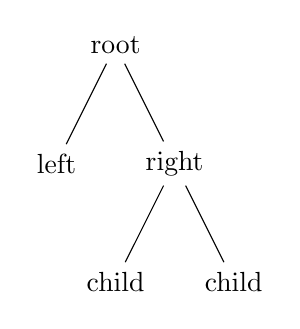
\begin{tikzpicture}
  \node {root}
    child {node {left}}
    child {node {right}
      child {node {child}}
      child {node {child}}
    };
\end{tikzpicture}

A simple image is \tikz \fill (0,0) circle(5pt);.
\end{document}
\end{codeexample}

The method works as follows: if the document is typeset normally, the library searches for replacement images for every picture. Filenames are generated automatically in the default configuration. In our case, the two file names will be |main-figure0| and |main-figure1|. If they exist, those images are simply included and the pictures as such are not processed. If graphics files do not exist, steps are taken to generate the missing ones. Since (currently) only one output file can be set, each missing image needs to be generated by a separate run of \LaTeX\ in which the |\jobname| is set to the desired image file name.
In the default configuration |mode=convert with system call|, these commands are issued automatically by using the |\write18| method to call system commands. It is also possible to output every required file name or to generate a |makefile|; users will need to issue the required commands manually (or with |make|). The probably most comfortable way is to use the default configuration with
\begin{codeexample}[code only]
pdflatex -shell-escape main
\end{codeexample}
\noindent which authorizes |pdflatex| to call itself recursively to generate the images. When it finishes, all images are generated and the document already includes them.


From this point on, successive runs of \LaTeX\ will use the final graphics files, the pictures won't be used anymore. Section~\ref{section-libs-external-nopgf} contains details about how to submit such a file to environments where \pgfname\ is not available.

\begin{command}{\tikzexternalize\oarg{optional arguments}}
	This command activates the externalization. It installs commands to replace every \tikzname-picture. It needs to be called before |\begin{document}| because it may need to install its separate shipout routine.


	The \meta{optional arguments} can be any of the keys described below.

	Note that the generation/modification of auxiliary files like |.aux|, |.toc| etc.\ is usually suppressed while a single image is externalized (details for |\label| support follow).

	It is also possible to write |\tikzexternalize|\marg{main job name} if the argument is delimited by curly braces. This case is mainly for backwards compatibility and is no longer necessary. Since it might be useful in rare circumstances, it is documented in section~\ref{sec:external:detail}.

	A detailed description about the process of externalization is provided in section~\ref{sec:external:detail}.

	\begin{command}{\tikzexternalrealjob}%
		After the library is loaded, this macro will \emph{always} contain the correct main job's name (in the example above, it is |main|). It is to be used instead of |\jobname| when the externalization is in effect.
	\end{command}
	\begin{command}{\pgfactualjobname}
		Once |\tikzexternalize| has been called, |\pgfactualjobname| contains the name of the currently generated output file (which may be |main| or |main-figure0| or |main-figure1| in our example above).
	\end{command}
	\begin{command}{\jobname}
		The value of |\jobname| is one of |\tikzexternalrealjob| or |\pgfactualjobname|, depending on the configuration. In short: if auxiliary file support (|\label| and |\ref|) is activated, |\jobname=\tikzexternalrealjob| (since that's the base file name of auxiliary files).
	\end{command}
\end{command}

\begin{key}{/tikz/external/system call=\marg{template}}
\label{extlib:systemcall:option}
	A template string used to generate system calls. Inside of \marg{template}, the macro |\image| can be used as placeholder for the image which is about to be generated while |\texsource| contains the main file name (in truth, it contains |\input|\marg{main file name}, but that doesn't matter).

	The default is
\begin{codeexample}[code only]
\tikzset{external/system call={pdflatex \tikzexternalcheckshellescape -halt-on-error
    -interaction=batchmode -jobname "\image" "\texsource"}
\end{codeexample}
	\noindent where \declareandlabel{\tikzexternalcheckshellescape} inserts the value of the configuration key |shell escape|
	if and only if the current document has been typeset with |-shell-escape|\footnote{Note that this is always true for the default configuration. This security consideration applies mainly for \texttt{mode=list and make} which will also work \emph{without} shell escapes.}.

	For |eps| output, you can (and need to) use
\begin{codeexample}[code only]
\tikzset{external/system call={latex \tikzexternalcheckshellescape -halt-on-error
    -interaction=batchmode -jobname "\image" "\texsource";
    dvips -o "\image".ps "\image".dvi}}
\end{codeexample}
	
	The argument \marg{template} will be expanded using |\edef|, so any control sequences will be expanded. During this evaluation, `|\\|' will result in a normal backslash, `|\|'. Furthermore, double quotes `|"|', single quotes `|'|', semicolons and dashes `|-|' will be made to normal characters if any package uses them as macros. This ensures compatibility with the |german| package, for example.
\end{key}

\begin{key}{/tikz/external/shell escape=\marg{command-line arg} (initially -shell-escape)}
	Contains the command line option for |latex| which enables the |\write18| feature. For \TeX-Live, this is |-shell-escape|. For Mik\TeX, you should use |\tikzexternalize[shell escape=-enable-write18]|.
\end{key}

\subsubsection{Support for Labels and References In External Files}
The |external| library comes with extra support for |\label| and |\ref| (and other commands which usually store information in the |.aux| file) inside of external files.

There are, however, some points which need your attention when you try to use
\begin{enumerate}
	\item[a)] |\ref| to something in the main document inside of an externalized graphics or
	\item[b)] |\label| in the externalized graphics which is referenced in the main document.
\end{enumerate}

For point a), a |\ref| inside of an externalized graphics works \emph{only} if you issue the required system call \emph{manually} or by |make|. The initial configuration |mode=convert with system call| does \emph{not} support |\ref|. But you can copy--paste the system call generated by |mode=convert with system call| and issue it manually. The reason is that |\ref| information is stored in the main |.aux| file -- but this auxiliary file is not completely written when |mode=convert with system call| is invoked (there is a race condition). Note that |\pageref| is not supported (sorry). Thus: if you have |\ref| inside of external graphics, consider using |mode=list and make| or copy--paste the system call for the image(s) and issue it manually.

Point b) is realized automatically by the external library. In detail, a |\label| inside of an externalized graphics causes the external library to generate separate auxiliary files for every external image. These files are called \meta{imagename}|.dpth|. The extension |.dpth| indicates that the file also contains the image's depth (the |baseline| key of \tikzname). Furthermore, anything which would have been written to an |.aux| file will be redirected to the |.dpth| file -- but only things which occur inside of the externalized |tikzpicture| environment. When the main document loads the image, it will copy the |.dpth| file into the main |.aux| file. Then, successive compilations of the main document contain the external |\label| information. In other words, a |\label| in an external graphics needs the following work flow:
\begin{enumerate}
	\item The external graphics needs to be generated together with its |.dpth| (usually automatically by \tikzname).
	\item The main document includes the external graphics and copies the |.dpth| content into its main |.aux| file.
	\item The main document needs to be translated one further time to re-read its |.aux| file\footnote{Note that it is not possible to activate the content of an auxiliary file after \texttt{\textbackslash begin\{document\}} in \LaTeX.}.
\end{enumerate}
There is just one special case: if a |\label|/|\ref| combination is realized itsself by a |tikzpicture| which should be externalized, you need to proceed as for case a) since |mode=convert with system call| can't handle that stuff on its own. Thus, |\label| works automatically, just translate the main document often enough.



\subsubsection{Customizing the Generated File Names}
The default filename for externalized graphics is `\meta{real file name}|-figure_|\meta{number}' where \meta{number} ranges from $0$ to whatever is required. However, there are a couple of ways to change the generated filenames:
\begin{itemize}
	\item Changing the overall file name using a |prefix|,
	\item Changing the file name for a single figure using |\tikzsetnextfilename|,
	\item Changing the file name for a restricted set of figures using |figure name|.
\end{itemize}

\begin{key}{/tikz/external/prefix=\marg{file name prefix} (initially empty)}
	A shortcut for |\tikzsetexternalprefix|\marg{file name prefix}, see below.
\end{key}

\begin{command}{\tikzsetexternalprefix\marg{file name prefix}}
	Assigns a common prefix used by all file names. For example,
\begin{codeexample}[code only]
\tikzsetexternalprefix{figures/}
\end{codeexample}
	will prepend |figures/| to every external graphics file name.

	Please note that |\tikzsetexternalprefix| is the \emph{only} way to assign a prefix in case you want to prepare your document for environments where \pgfname\ is not installed (see section~\ref{section-libs-external-nopgf}).
\end{command}

\begin{command}{\tikzsetnextfilename\marg{file name}}
	Sets the file name for the \emph{next} \tikzname\ picture or |\tikz| short command. It will \emph{only} be used for the next picture.

	Pictures for which no explicit file name has been set (or the next file name is empty) will get automatically generated file names.

	Please note that |prefix| will still be prepended to \marg{file name}.
\begin{codeexample}[code only]
\documentclass{article}
% main document, called main.tex
\usepackage{tikz}

\usetikzlibrary{external}
\tikzexternalize[prefix=figures/] % activate

\begin{document}

\tikzsetnextfilename{trees}
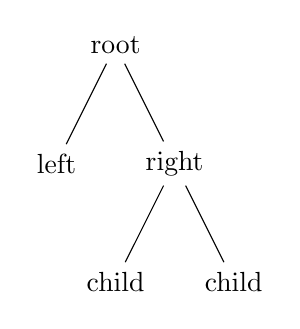
\begin{tikzpicture} % will be written to 'figures/trees.pdf'
  \node {root}
    child {node {left}}
    child {node {right}
      child {node {child}}
      child {node {child}}
    };
\end{tikzpicture}

\tikzsetnextfilename{simple}
A simple image is \tikz \fill (0,0) circle(5pt);. % will be written to 'figures/simple.pdf'


\begin{tikzpicture} % will be written to 'figures/main-figure0.pdf'
   \draw[help lines] (0,0) grid (5,5);
\end{tikzpicture}
\end{document}
\end{codeexample}
\begin{codeexample}[code only]
pdflatex -shell-escape main
\end{codeexample}
\end{command}

\begin{key}{/tikz/external/figure name=\marg{name}}
	Same as |\tikzsetfigurename|\marg{name}.
\end{key}
\begin{command}{\tikzsetfigurename\marg{name}}
	Changes the names of \emph{all} following figures. It is possible to change |figure name| during the document either using |\tikzset{external/figure name|=\marg{name}|}| or with this command. A unique counter will be used for each different \marg{name}, and each counter will start at $0$.

	The value of |prefix| will be applied after |figure name| has been evaluated.
\begin{codeexample}[code only]
\documentclass{article}
% main document, called main.tex
\usepackage{tikz}

\usetikzlibrary{external}
\tikzexternalize % activate

\begin{document}

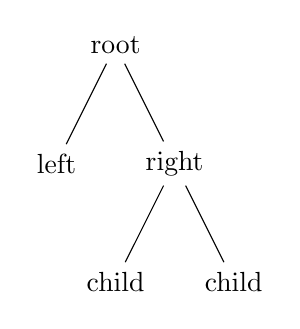
\begin{tikzpicture} % will be written to 'main-figure0.pdf'
  \node {root}
    child {node {left}}
    child {node {right}
      child {node {child}}
      child {node {child}}
    };
\end{tikzpicture}

{
  \tikzsetfigurename{subset_}
  A simple image is \tikz \fill (0,0) circle(5pt);. % will be written to 'subset_0.pdf'

  
\begin{tikzpicture} % will be written to 'subset_1.pdf'
     \draw[help lines] (0,0) grid (5,5);
  \end{tikzpicture}
}% here, the old file name will be restored:

\begin{tikzpicture} % will be written to 'main-figure1.pdf'
   \draw (0,0) -- (5,5);
\end{tikzpicture}
\end{document}
\end{codeexample}
	The scope of |figure name| ends with the next closing brace.

	Remark: Use |\tikzset{external/figure name/.add={prefix_}{_suffix_}}| to add a |prefix_| and a |_suffix_| to the actual value of |figure name|.
\end{command}

\begin{command}{\tikzappendtofigurename\marg{suffix}}
	Appends \meta{suffix} to the actual value of |figure name|.

	It is a shortcut for |\tikzset{external/figure name/.add={}|\marg{suffix}|}| (a shortcut which is also supported if \tikzname\ is not installed, see below).
\end{command}


\subsubsection{Remaking Figures or Skipping Figures}
\begin{command}{\tikzpicturedependsonfile\marg{file name}}
	Adds a dependency for the \emph{next} picture which is about to be externalized. If the command is invoked within a picture environment, it adds a dependency for the surrounding picture. Dependencies are written into \meta{target file}|.dep| in the format
	
	\meta{target file}|.\tikzexternalimgextension: |\meta{file name}.

	The effect is that if \meta{file name} changes, the external graphics associated with the picture shall be remade.

	This command uses the contents of \declareandlabel{\tikzexternalimgextension} to check for graphics. If you encounter difficulties with image extensions, consider redefining this macro (after |\tikzexternalize|).

	\paragraph{Limitations:} this command is currently only supported for |mode=list and make| and the generated |makefile|.
\end{command}
\begin{command}{\tikzexternalfiledependsonfile\marg{external graphics}\marg{file name}}
	A variant of |\tikzpicturedependsonfile| which adds a dependency for an \meta{external graphics}. The argument \meta{external graphics} must be the path as it would have been generated by the external library, i.e.\ without file extension but including any prefixes.
\end{command}

\begin{key}{/tikz/external/force remake=\marg{boolean} (default true)}
	A boolean which is used to customize the up-to-date checks of all following figures. Every up-to-date check will fail, resulting in automatic regeneration of every following figure.

\begin{codeexample}[code only]
\tikzset{external/force remake}

\begin{tikzpicture}
	\draw (0,0) circle(5pt);
\end{tikzpicture}
\end{codeexample}
	You can also use |force remake| inside of a local \TeX\ group to remake only selected pictures. The example
\begin{codeexample}[code only]
\tikz \draw (0,0) -- (1,1);

{
\tikzset{external/force remake}

\begin{tikzpicture}
   \draw (0,0) circle(5pt);
\end{tikzpicture}
}

\tikz \draw (0,0) -- (1,1);
\end{codeexample}
	will only apply |force remake| to the second figure.

	Up-to-date checks are applied for |mode=convert with system call| and the makefile generated by |mode=list and make|.
\end{key}

\begin{key}{/tikz/external/remake next=\marg{boolean} (default true)}
	A variant of |force remake| which applies only to the next image.
\end{key}

\begin{key}{/tikz/external/export next=\marg{boolean} (default true)}
	A boolean which can be used to disable the export mechanism for single pictures.
\end{key}

\begin{key}{/tikz/external/export=\marg{boolean} (initially true)}
	A boolean which can be used to disable the export mechanism for all pictures inside of the current \TeX-scope.

\begin{codeexample}[code only]
\begin{document}
\begin{tikzpicture} % will be exported
	...
\end{tikzpicture}

{
\tikzset{external/export=false}
\begin{tikzpicture} % won't be exported
	...
\end{tikzpicture}
...
}

\begin{tikzpicture} % will be exported
	...
\end{tikzpicture}
\end{document}
\end{codeexample}
	For \LaTeX, the feature lasts until the next |\end|\marg{$\cdot$} (this holds for every call to |\tikzset|).
\end{key}

\begin{command}{\tikzexternaldisable}
	Allows to disable the complete externalization. While |export next| will still collect the contents of picture environments, this command uninstalls the hooks for the external library completely. Thus, nested picture environments or environments where |\end{tikzpicture}| is not directly reachable won't produce compilation failures -- although it is not possible to externalize them automatically.

	The externalization remains disabled until the end of the next \TeX\ group (or environment) or until the next call to |\tikzexternalenable|.
\end{command}

\begin{command}{\tikzexternalenable}
	Re-enables a previously running externalization after |\tikzexternaldisable|.
\end{command}


\subsubsection{Customizing the Externalization}
\begin{key}{/tikz/external/figure list=\marg{boolean} (initially true)}
	A boolean which configures whether a figure list shall be generated. A figure list is an output file named \marg{jobname}|.figlist| which is filled with file names of each figure, one per line.

	This file is not used by \TeX\ anymore, its purpose is to issue the required conversion commands |pdflatex -jobname |\marg{picture file name} \marg{main file} manually (or in a script). See section~\ref{sec:external:detail} for the details about the expected system call (or activate |mode=convert with system call| and inspect you log file).

\begin{codeexample}[code only]
\documentclass{article}
% main document, called main.tex
\usepackage{tikz}

\usetikzlibrary{external}
\tikzexternalize[
   mode=graphics if exists,
   figure list=true,
   prefix=figures/]

\begin{document}

\tikzsetnextfilename{trees}
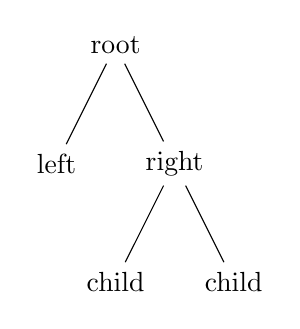
\begin{tikzpicture}
  \node {root}
    child {node {left}}
    child {node {right}
      child {node {child}}
      child {node {child}}
    };
\end{tikzpicture}

\tikzsetnextfilename{simple}
A simple image is \tikz \fill (0,0) circle(5pt);.


\begin{tikzpicture}
   \draw[help lines] (0,0) grid (5,5);
\end{tikzpicture}
\end{document}
\end{codeexample}

\begin{codeexample}[code only]
pdflatex main
\end{codeexample}
generates |main.figlist| containing
\begin{codeexample}[code only]
figures/trees
figures/simple
figures/main-figure0
\end{codeexample}
\end{key}

\begin{key}{/tikz/external/mode=\marg{choice} (initially convert with system call)}
	Configures what to do with \tikzname\ pictures (unless we are currently externalizing one particular image, in that case, these modes are ignored).

	The preconfigured mode |convert with system call| checks whether external graphics files are up-to-date and includes them if that is the case. Any picture which is not up-to-date will be generated automatically using a system call. The system call can be configured using the |system call| template. The up-to-date check is simple: if the file does not exist, it is not up-to-date. Furthermore, if one of the |force remake| or |remake next| keys is true, the figure is not up-to-date. In all other case, the file is considered to be up-to-date. As soon as |convert with system call| is set, the |figure list| will be disabled -- such a file is not required. In case you still need or want it, you can enable it after setting |mode|.

	Please note that system calls may be disabled for security reasons. For pdflatex, they can be enabled using
\begin{codeexample}[code only]
pdflatex -shell-escape
\end{codeexample}
	while other \TeX\ variants may need other switches. The feature is sometimes called |\write18|.
	
	The choice |only graphics| always tries to replace pictures with external graphics. It is an error if the graphics file does not exist.

	The choice |no graphics| (or, equivalently, |only pictures|) typesets \tikzname\ pictures without checking for external graphics.

	A mixture is |graphics if exists|, it checks whether a suitable graphics file exists and includes it if that is the case. If it does not exist, the picture is typeset using \TeX.

	Mode |list only| skips every \tikzname\ picture; it only generates the file \marg{main file}|.figlist| containing file names for every picture, the contents of any picture environment is thrown away and a replacement text is shown. This implies |figure list=true|. See also the |list and make| mode which includes available graphics.

	The mode |list and make| is similar to |list only|: it generates the same file \marg{main file}|.figlist|, but any images which exist already are included as graphics instead of ignoring them. Furthermore, this mode generates an additional file: \marg{main file}.makefile. This allows to use a work flow like
\begin{codeexample}[code only]
% step 1: generate main.makefile:
pdflatex main
% step 2: generate ALL graphics on 2 processors:
make -j 2 main.makefile
% step 3: include the graphics:
pdflatex main
\end{codeexample}
	\noindent This last make method is, however unnecessary: |list and make| just assumes that images are generated somehow (not necessarily with the generated makefile). The generated makefile allows parallel externalization of graphics on multi-core systems and it supports any file dependencies configured with |\tikzpicturedependsonfile|. Furthermore, it respects the |force remake| and |remake next| keys.


\end{key}


\begin{key}{/tikz/external/verbose IO=\marg{boolean} (initially true)}
	A boolean which configures whether I/O operations shall be listed in the logfile.
\end{key}
\begin{key}{/tikz/external/verbose optimize=\marg{boolean} (initially true)}
	A boolean which configures whether optimization operations shall be listed in the logfile.
\end{key}
\begin{key}{/tikz/external/verbose=\marg{boolean} (initially true)}
	Sets all verbosity flags to \meta{boolean}.
\end{key}

\begin{key}{/tikz/external/optimize=\marg{boolean} (initially true)}
	Configures whether the conversion process shall be optimized. This affects only the case when |\jobname| differs from the main file name, i.e. when single pictures are converted.

	In that case, the main file is compiled as usual - but everything except the selected picture is thrown away. If optimization is enabled, all other pictures won't be processed at all. Furthermore, expensive commands which do not contribute to the selected picture will be thrown away as well.

	The default implementation discards |\includegraphics| commands which are \emph{not} inside of the selected picture to reduce conversion time.

	It is possible to add commands which shall be optimized away, see below.
\end{key}

\begin{key}{/tikz/external/optimize command away=\meta{\textbackslash command}\marg{required argument count}}
	Installs commands to optimize \meta{\textbackslash command} away. As is described above, optimization applies to the case when single pictures are converted: one usually doesn't need to process (probably expensive) commands which do not contribute to the selected picture.

	The argument \marg{required argument count} is either empty or a non-negativ integer between $0$ and $9$. It denotes the number of arguments which should be consumed after \meta{\textbackslash command}. In any case, one argument in square brackets after the command will be recognized as well. To be more precise, the following cases for arguments of \meta{\textbackslash command} are supported:
	\begin{enumerate}
		\item If \marg{required argument count} is empty (the default), \meta{\textbackslash command} may take one optional argument in square brackets and one in curly braces (which is also optional).
		\item If \marg{required argument count} is not empty, \marg{\textbackslash command} may take one optional argument in square brackets. Furthermore, it expects exactly \marg{required argument count} following arguments.
	\end{enumerate}

	Example:
\begin{codeexample}[code only]
\tikzset{external/optimize command away=\includegraphics}
\end{codeexample}

\begin{codeexample}[code only]
\newcommand{\myExpensiveMacro}[1]{Very expensive!}

\tikzset{external/optimize command away=\myExpensiveMacro}
\end{codeexample}

\begin{codeexample}[code only]
\newcommand{\myExpensiveMacroWithThreeArgs}[3]{Very expensive!}

\tikzset{external/optimize command away={\myExpensiveMacroWithThreeArgs}{3}}
\end{codeexample}
\begin{codeexample}[code only]
% A command with optional argument:
\newcommand{\aFurtherExample}[3][]{Very expensive!}

% consume only two arguments: the first optional one will be processed
% anyway:
\tikzset{external/optimize command away={\myExpensiveMacroWithThreeArgs}{2}}
\end{codeexample}
	The argument \meta{\textbackslash command} must be the name of a single macro. Any occurrence of this macro, together with its arguments, will be removed.
\begin{codeexample}[code only]
\begin{tikzpicture}
	% this picture is currently converted!
\end{tikzpicture}

This here is outside of the converted picture and contains \myExpensiveMacro. It will be discarded.

This call: \myExpensiveMacro[argument=value]{Argument} as well.
And this here: \myExpensiveMacro{Argument} also.
\end{codeexample}

	The default is to optimize |\includegraphics| away.

	This key is actually a style which sets the |optimize/install| and |optimize/restore| keys.
\end{key}

\begin{key}{/tikz/external/optimize/install}
	A command key which contains code to install optimizations. You can append code here (or clear the macro) if you need to modify the optimization.
\end{key}
\begin{key}{/tikz/external/optimize/restore}
	A command key which contains code to undo optimizations. You can append code here (or clear the macro) if you need to modify the optimization.
\end{key}

\begin{key}{/tikz/external/only named=\marg{boolean} (initially false)}
	If enabled, only pictures for which file names have been set explicitly using |\tikzsetnextfilename| will be considered, no file names will be generated automatically.
\end{key}

\begin{key}{/pgf/images/include external (initially \textbackslash pgfimage\{\#1\})}
\index{External Graphics!Bounding Box Issues}
	This command key constitutes the public interface to exchange the |\includegraphics| command used for the image inclusion. If can be overwritten using |include external/.code=|\marg{\TeX\ code}.

	Its description can be found in the corresponding basic layer documentation on page~\pageref{pgf:includeexternalkey}.

	Just one example here: you can use
\begin{codeexample}[code only]
\pgfkeys{/pgf/images/include external/.code={\includegraphics[viewport=0 0 211.28 175.686]{#1}}}
\end{codeexample}
	to manually change the viewport (bounding box) for included graphics.

	Another example (of probably limited use) is
\begin{codeexample}[code only]
\pgfkeys{/pgf/images/include external/.code={\href{file:#1}{\pgfimage{#1}}}}
\end{codeexample}
	\noindent which will generate a clickable hyperlink around the image. Clicking on it opens the single exported file\footnote{This requires all external graphics files in the same base directory as the main |.pdf| file.}.
	
	If you want to limit the effects of this key to just one externalized figure, use
\begin{codeexample}[code only]
{
  \pgfkeys{/pgf/images/include external/.code={\includegraphics[viewport=0 0 211.28 175.686]{#1}}}
  \begin{tikzpicture}
     ...
  \end{tikzpicture}
}% this brace ends the effect of `include external'
\end{codeexample}
\end{key}

\begin{command}{\tikzifexternalizing\marg{true code}\marg{false code}}
	This command can be used to check whether an image is currently written to its separate graphics file (if the ``grab'' procedure is running). If so, the \marg{true code} will be executed. If not, that means if the main document is being typeset normally, the \marg{false code} will be invoked.

	This command must be used \emph{after} |\tikzexternalize|.
\end{command}

\begin{command}{\tikzifexternalizingnext\marg{true code}\marg{false code}}
	Like |\tikzifexternalizing|, but this variant also checks if the next following figure is the one which is about to be written to its separate graphics file.
\end{command}

\subsubsection{Details About The Process}
\label{sec:external:detail}
The standard run |pdflatex |\meta{main document} causes the |external| library to check every occurrence of |\begin{tikzpicture}| and every |\tikz| shortcommand. If it finds a picture which shall be exported, it queries the respective file name and checks whether the file exists already. If so, it includes the external graphics. If not, it requires an externalization which can be done automatically (the default), semi--automatically (with |mode=list and make|) or manually (by issuing the requires system calls somehow).

The library can detect whether it runs in ``conversion mode'', i.e.\ if it should only process a single image. To do so, it checks whether the internal macro \declareandlabel{\tikzexternalrealjob} exists. If so, its contents is assumed to be \meta{main document} (without the suffix |.tex|). Usually, this macro is set by the conversion system call,
\begin{codeexample}[code only]
pdflatex -jobname "main-figure0" "\def\tikzexternalrealjob{main}\documentclass[mai, 10pt, english, crop, info, print]{liuthesis}

% Pasted from Niklas main.tex
      \usepackage{amsmath,amssymb}
      \usepackage[table]{xcolor}
      %\usepackage{makeidx}
      \usepackage{savesym}
      \savesymbol{AND}
      %\usepackage{algorithmic}
      \usepackage{algorithm}
      %\usepackage{tikz}
      \usepackage{pdfpages}
      \usepackage{subfigure}
      \usepackage{graphicx}
      \usepackage{algpseudocode}
      \usepackage{algorithmicx}
      %\usepackage{hyperref}
      
      %\usetikzlibrary{positioning,chains,fit,shapes,calc}


      \DeclareMathOperator{\diag}{diag}
      \DeclareMathOperator{\rank}{rank}
      \newcommand{\x}{\times}
      \newtheorem{proposition}[theorem]{Proposition}
%

\author{Abhijith Chandraprabhu}
\title{Collaborative Filtering using Temporal Analysis}{Svenk Titel}

\thesisDate{9}{19}{YYYY}
\thesisNo{LiTH-MAT-EX{-}{-}YY/XXXX{-}{-}SE}

\thesisDivision{Division of Applied Mathematics}
\URL[http://math.liu.se]{http://www.ep.liu.se}

\subject{Department of Mathematics}
\keywords{Netflix, Recommender Systems, RMSE, Matrix factorization, Sparse SVD,
ALS-WR, Low-Rank Approximation,}

\examiner{
  Lars Eld�n \AT \textsc{mai}, Link�pings universitet}

\supervisor{
  Berkant Savas \AT \textsc{mai}, Link�pings universitet}

\abstract{In todays digital world Information in the form of large scale data
has become a very important source of knowledge, this is largely owed to the
advances in Data Sciences. One of the recent applications of data mining is to
find meaningful and useful relationship between groups of entities, for
example between users and movies as in the case of NETFLIX. With the NETLIX
competition, the field of Recommender Systems which helps in presenting users
with relevant items based on the history rather than an explicit search query,
has generated great interest from researchers and this work is one such attempt.
When we talk about users' preferences it is natural that it evolves, hence in
this work we have tried to account for a new dimension, i.e time, while building
the model. On the lines on the NETFLIX competition, the task of predicting
preferences involves the ratings of the movies given by users and it is the
value of this rating which we try to predict. On the lines on the NETFLIX
competition, the task of predicting preferences involves the ratings of the
movies by users and it the value of this rating which we try to predict. The
data upon which the algorithm is built consists of around 1 million ratings
given by around half a million users to around 18k movies. Collaborative
Filtering techniques have been employed, where based upon a model which has
information of users and movies we try to fetch prediction of new ratings by
factoring the user space and movie space and finding a relationship between the
required pair. Matrix factorization is done based on Singular Value
Decomposition, and owing to the inherent nature of SVD to handle
sparse data inefficiently an alternate method based on Alternate Least Squares
was used.}

\acknowledgements{ Parents, Berkant Savas, Lars Elden, Niklas Ekvall, Opposition person.}
%\useHyperRef

\begin{document}

\makeFrontMatter

\chapter{Introduction\index{Introduction}}


\textsf{%
In this chapter we introduce the field of Datamining and its relevance. We
also introduce the area of research in which this thesis work is done.}

\section{Introduction\index{Introduction}}
The field of Data Mining aka Knowledge Discovery in Data, or KDD saw its first
light during the 1990s, and has evolved along with the processing power and
storage capacities of modern computer systems. The amount of data only from the
web is in the order of exabytes and continues to increase, this along with other
sources of data resulting from reserach and experimentation proves to be one the
most important sources of knowledge. The data mining techniques are applied
to wide variety of applications like in business, to improve customer
relationhip management, or to do market analysis with respect to a particular
product. The medical fraternity use them to do temporal analysis of patterns
concerning drug presciptions to diagnoses. With respect to science and
engineering, DNA sequence mining proves very crucial in understanding the
variations in human DNA. Data mining actually can be seen as one step towards
discovering knowledge from raw source, initially there are many more processes
like understanding of the application domain and collecting the data, then there
is data transformation and only then is the actual data mining techniques
applied. Even after the data is mined and clusters or patterns are obtained,
interpretation of these patterns and taking required actions forms the last
stage. There are six main tasks within the gamut of data mining, enlisted
below, \cite{Fayyad96fromdata}
\begin{description}
  \item[Classification] is learning a function that maps a data item into one of
several predefined classes.
  \item[Regression] is learning a function that maps a data item to a
real-valued prediction variable.
  \item[Clustering] is a common descriptive task where one seeks to identify a
finite set of categories or clusters to describe the data.
  \item[Summarization] involves methods for finding a compact description for a
subset of data.
  \item[Dependency Modeling] consists of finding a model that describes
significant dependencies between variables.
\item[Change and deviation detection] focuses on discovering the most
significant changes in
the data from previously measured or normative values.
\end{description}

  The kind of prediction we are dealing with is ratings prediction, which gives
an indication of user's preference to items. Depending on the predicted rating
recommendations are made, this involves different tasks the most significant of
them being matrix factorization and rank reduction. It is very common while
dealing with preferences that they tend to change with time, the work by
\cite{Koren:2010:CFT:1721654.1721677} models the data drifting with time. It is
important to note that while modeling temporal effects we should take into
account there are transient signals analogous to users and a more long term
patterns characterized by movies.



\chapter{Collaborative Filtering\index{Collaborative Filtering}}


\textsf{ In this chapter we explain Collaborative Filtering in more detail,
along with giving details of the NETFLIX prize and the lead up to present work.
We explain about the data and the approach to the solution of the problem.}


\section{Recommender Systems\index{Recommender Systems}}
Internet technologies have greatly become a part of our lives, there are many
occasions when we need help in taking certain decisions. Recommendations in
general is ubiquitous when there is a need to make choices without sufficient
personal experience, we rely on feedback from users on certain products, we make
use of recommendation letters for jobs, reviews of movies and books
\cite{Resnick:1997:RS:245108.245121}. Consider for a movie streaming company
like NETFLIX, where people can watch movies from a huge collection, have been
collecting the ratings of the movies from the users. This data can be considered
as our \emph{training data}, it is explicitly obtained from the users. Using
this training data the company makes predicitions of movies the users are likely
to prefer watching more than others. This is only one of the different types of
recommender systems. 
\subsection{Recommender System Strategies}
The strategies for building recommender systems are based on the type of data
available and how the data is used. On a broad sense the two main approaches are
\emph{content-based filtering}, in which the items are characterized based on 
certain attributes, and recommendation are made based on filtering similar
items. In the second approach, \emph{collaborative filtering}, the ratings
previously given by users is used to build a model, which is then used to make
predictions. The term Collaborative Filtering was first termed by Tapestry
\cite{Goldberg:1992:UCF:138859.138867}, which was one of the first recommender
systems. Recommender
Systems produce possibly accurate prediction of relationship between elements of
different classes based on previous knowledge or the \emph{training data}. This
training data could be explicitly obtained in the form of ratings given by
users or it could be implicit knowledge(purchase
history, browsing history, search patterns,mouse movements etc), which can be
used when explicit knowledge is insufficient \cite{Hu:2008:CFI:1510528.1511352}.
But however in this thesis work we model our system based on explicit
knowledge. 

Modern recommender systems are based on the collaborative filtering, which again
is of two types, the \emph{nearest neighbor approach} and the \emph{latent
factor approach}. In the nearest neighbor methods, items or users are given
certain attributes which decides the proximity between them. Further this sense
of proximity is used predict an item for an user. The second approach is
the latent factor approach, which characterizes the users and the items together
in building the model. Matrix factorization is used to build these models, likes
of SVD is very useful. \emph{Rating matrix} proves to be important, as it
charectarizes both items and users as its vectors. 

\subsection{The Problem Formulation}
Our problem could be defined as a matrix completion problem, where the matrix is
formed by placing the users $u$ along the rows and the movies $m$ along the
rows. The entries in this matrix are filled through the \emph{training data},
which is collection of $n$ \emph{quadruples}, with the format
(\emph{user(k)},\emph{movie(k)},\emph{rating(k)},\emph{timestamp(k)}), where
$k=1,2...,n$. The $1 \leq user \leq u$ and $1 \leq movie \leq m$ are the
range of the users and the movies, where as the ratings, $1<rating<5$. The
\emph{Rating
matrix} is defined as $R\in\mathbb{R}^{u,m}$, \\
\begin{equation}
  R[i,j]=\begin{cases}
    rating(k), & \text{$i=user(k), j=movie(k)$}.\\
    ?, & \text{otherwise}.
  \end{cases}
\end{equation}

where \emph{'?'} are the cases where the \emph{user-movie} relation is unknown.
These are the values which needs to be predicted. Once the \emph{'?'} values are
computed, recommendations could be made depending on the required tolerance
level, \emph{user-movie} pairs with predicted ratings higer than the tolerant
value(threshold) can be selected for making recommendations. Hence this problem
can be viewed as a \emph{matrix completion} problem. In this thesis work, we
will compute the unknowns for a certain subset called the \emph{test set}. \\

Let us denote the completed matrix, or rather the reconstructed matrix	 by
\emph{$\hat_{R}$}. We intend to obtain the
\emph{$\hat_{R}$}, by reproducing it through a simple product of two matrices
with reduced \emph{inner dimension}. Let $P\in\mathbb{R}^{u,f}$ and
$Q\in\mathbb{R}^{f,m}$ are the two matrices with reduced inner dimension
\emph{f}. 


Let us through a very simple example see the principle behind collaborative
filtering.

 \begin{example}
   We show 4 users who have rated 4 movies, we tabulate the preferences, in the
form of ratings on the scale of 1 to 5,  as shown below. The users are along the
rows and items along the columns, rating  given by \textit{user i} to
\textit{item j} is the real valued entry (i,j) in  the rating matrix.  \\

\begin{tabular}{c|cccc}
       & Titanic & Braveheart & The Lion King & Dreamcatcher  \\
\hline
John   & 5 & 5 & 2 & -   \\
Dave   & 2 & - & 3 & -   \\
Alice  & - & 5 & - & 3   \\
Bob    & 3 & - & - & 5   \\
\end{tabular}

From the above, we can consider the rating matrix to be \\

$R_{i,j}$ =
$ \begin{pmatrix}
  5 & 5 & 2 & ? \\
  2 & ? & 3 & 5 \\
  ? & 5 & ? & 3  \\
  3 & ? & ? & 5
 \end{pmatrix} $\\
 
 Using matrix factorization, we simply do a SVD on $R$ to get, $U$ and $V$,
which denote the user space and the movie space. \\
 
 $U$ =
 $\begin{pmatrix}
  1.12 & 1.49 & 0.48  \\
  1.31 & -0.52 & 0.59  \\
  1.13 & 0.67 & -0.52  \\
  1.39 & 0.05 & 0.45 
 \end{pmatrix} $
 \hspace*{10mm}
 $V$ =
 $\begin{pmatrix}
  1.12 & 1.49 & 0.48  \\
  1.31 & -0.52 & 0.59  \\
  1.13 & 0.67 & -0.52  \\
  1.39 & 0.05 & 0.45 
 \end{pmatrix} $\\

 Once we have factored the rating matrix $R$, we can get the missing values by
approximating the sparse rating matrix into a full one,  $\hat{R}=U*V'$ \\

$\hat{R}_{i,j}$ =
 $\begin{pmatrix}
  4.78 & 4.98 & 1.97 & 3.61 \\
  1.98 & 1.97 & 2.85 & 4.81 \\
  2.75 & 4.71 & 1.40 & 2.94  \\
  2.94 & 3.32 & 2.75 & 4.79
 \end{pmatrix} $\\
 
 With this approximation, we can make predictions of ratings of movies which the
users have not seen. 
 
\end{example}

\section{NETFLIX}
Entertainment has been one of the most significant integral part of human
society and has evloved along with modern technologies. In todays internet
driven society, IPTV(Internet Protocol Television) is gaining popularity in
delivering television and cinema content to viewers. IPTV mainly consists of
three groups, \\
\begin{enumerate}%for small alpha-characters within brackets.
\item Live Television - Live telecast or transmission to the viewers with only
the transmission delay, example live news show.
\item Time-shifted Television which is also called as catch-up TV, in which the
viewers can watch the content which is stored and available at any point of
time. 
\item Video on Demand - here the viewers are given a wide range of TV shows and
movies to choose. They can watch anything they wish, the content is streamed to
the viewers computer which the user can pause and watch later. NETFLIX provides
its content throught this method. \\
This owes to a great extent to the success of NETFLIX, since through on Demand
system NETFLIX is able to cater to individual tastes of users. NETFLIX can
collect statistics pertaining to individual users' choices and the most
important metric is the \emph{ratings}. NETFLIX aims to greatly improve the
customer satisfaction and retention by providing a greatly personalised
experience to the users. The importance of personalization is such, that NETFLIX
ignited the research attempts in the Mathematical and Computer Science soceity
to develop methods which could do predictions for movie likeability quotient.
Such attempts have certainly been fruitful to NETFLIX as is evident from the
fact that as of today 33 million members view over 1 billion hours of TV shows
and movies through NETFLIX per month.
\end{enumerate}

\subsection{NETFLIX Prize}
During October 2006, NETFLIX challenged the research community to beat the
performance in terms of accuracy of their own recommendation system
\emph{Cinematch} by 10\%. The NETFLIX prize challenge was provided with over 100
million ratings from around half a million users and 18 thousand movies. This
data was collected during the period october 1998 and December 2005. The
challenge would take place over a period of three years, and a progress prize of
50 thousand USD would be awarded each year to the team which would produce the
best improvements. Finally at the end of three years a Grand Prize of 1 Million
USD would be given to the team with the best results in terms of RMSE. Their
benchmark system \emph{Cinematch}, based on \emph{Pearson correlation} which is
straightforward statistical linear model produces an RMSE of 0.9525 on test
data. Hence to qualify to win the Grand Prize which accounts for 10\%
improvement over \emph{Cinematch}, which corresponds to RMSE of 0.8563 on
\emph{quiz set}. On an event of a tie the time of entry would be taken into
account, and this is exactly what happened on 26 July 2009, team BellKor's
Pragmatic Chaos won the challenge by margin of 20 minutes. Table 2.1 shows the
performance of top 12 teams, \cite{NETFLIX_Prize:Online}
\begin{table}
\centering 
\begin{tabular}{|c|c|c|c|} \hline %\hline
%-------------------------------------------------------------------
$Rank$ & $Team$ & 
$RMSE$ &  $Percent Improvement$  \\ 
\hline
%-------------------------------------------------------------------
$ 1$
& $BellKor's Pragmatic Chaos$
& $0.8567$
& $10.06$ \\ %\hline
%-------------------------------------------------------------------
$ 2$
& $The Ensemble$
& $0.8567$
& $10.06$ \\ %\hline
%-------------------------------------------------------------------
$ 3$
& $Grand Prize Team$
& $0.8582$
& $9.90$\\  %\hline
%-------------------------------------------------------------------
$ 4$
& $Opera Solutions and Vandelay United$
& $0.8588$
& $9.84$\\  %\hline
%-------------------------------------------------------------------
$ 5$
& $Vandelay Industries !$
& $0.8591$
& $9.81$ \\%\hline
%-------------------------------------------------------------------
$ 6$
& $PragmaticTheory$
& $0.8594$
& $9.77$ \\ %\hline
%-------------------------------------------------------------------
$ 7$
& $BellKor in BigChaos$
& $0.8601$
& $9.70$ \\ %\hline
%-------------------------------------------------------------------
$ 8$
& $Dace$
& $0.8612$
& $9.59$ \\ %\hline
%-------------------------------------------------------------------
$ 9$
& $Feeds2$
& $0.8622$
& $9.48$  \\%\hline
%-------------------------------------------------------------------
$ 10$
& $BigChaos$
& $0.8623$
& $9.47$ \\ %\hline
%-------------------------------------------------------------------
$ 11$
& $Opera Solutions$
& $0.8623$
& $9.47$ \\ %\hline
%-------------------------------------------------------------------
$ 12$ 
& $BellKor$        
& $0.8624$ 
& $9.46$  \\ \hline 
\end{tabular}
\caption{RMSE of Top 12 Teams}
\label{tab:TopTeams}
\end{table}
-
\subsection{The NETFLIX dataset}
NETFLIX had been collecting data since October 1998,
as of June 2007 the company had collected over 1.9 billion ratings from more
than 11.7 million subscribers over 85 thousand titles \refname{The NETFLIX
Prize}. The company then recieved over 2 million ratings per day. To provide
data for the competition the company did two seperate random sampling processes,
the first one to obtain th eentire Prize dataset and second for the qualifying
and probe set. The condition for selecting the users was that they should have
given minimum of 20 ratings. \\

 Basically the company has seggregated the data based on time, the latest data
form the Test Data and the initial data form the training data. The
\emph{Training data} includes the \emph{Probe set} which is meant for fine
tuning before submissions. The training data is basically a text file consisting
of triplets entries like, (UserID, MovieID, Rating). There are 100 million such
entries which form the training set. The training set also included the probe
set consisting of 1,408,395 triplets, this could be used by the competitors to
fine tune their algorithms before submission. NETFLIX also collected the latest
ratings of all the users in the training set to form the \emph{Qualifying set}.
This set was in the form (UserID,MovieID,DatrofRating), where the ratings were
known only to the judjes. The qualifying set was again divided into 2 groups,
the \emph{Quiz set} and \emph{Test set}. The quiz set having 1,408,342 ratings
was used to update the Leaderboard, the RMSE on this quiz set was released to
the competitors. The test set having 1,408,789 ratings was only used by the jury
to adjudge the winner. \cite{Bennett07thenetflix}\\



 
\begin{table}
\begin{center}
    \begin{tabular}{|ccc|}
        \hline
         TRAINING SET  & ~ &  Probe set  \\ 
         100480507 & ~ & 1408395   \\ \hline       
    \end{tabular} \\
    \caption[]{Training Data}
     \begin{tabular}{|c|c|}
       \hline
       Test Set  & Quiz Set  \\ 
       1408789 & 1408342 \\ \hline       
    \end{tabular}
    \caption{Qualifying Data}     
\end{center}
\end{table}


\section{Matrix Factorization for Collaborative Filtering}
With Collaborative Filtering it involves filtering for information through
collaboration among interacting groups, for example users and movies. Matrix
factorization happens to be the first choice for collaborative filtering, as
matrices can hold high dimensional information in tabular form, and can be
factored into products of smaller matrices. \emph{In matrix factorization the
users and items are mapped onto a joint latent factor space of reduced dimension
$f$, and the inner product of the user vector with item vector gives the
corresponding interaction.} \cite{Koren:2009:MFT:1608565.1608614}
\subsection{Basic Matrix Factorization}
Matrix factorization is mainly about a more compact representation of the large
training data which is obtained by dimensionality reduction.
\cite{Liu:2010:GLA:1821715.1821722}. 
\emph{We want to quantify the nature or the characteristics of the movies
defined by a certain number of aspects (factors), i.e we are trying to
generalize the information (independent and unrelated ratings matrix) in a
concise and descriptive way.} \cite{citeulike:4563139} All the movies can be
described by certain features like overall rating, cast, wether its an action
flick or romantic drama, how did it fare during the first week of it release
etc. Similarly a user can also be described based on the same factors, wether
the user is liberal in rating or very critical, does the user have certain
favourite cast, if the user prefers action over romance, does the user watch and
rate movies on the first week of its release etc. What we have here is a common
factor space in which we tend to generalize the relationships between the users
and movies, based on these factors. Hence the 8.5 billion ratings can be
explained in lot fewer factors. We are generalizing the independent individual
unrelated ratings to a more concise and descriptive form. Here what we have done
is through meaningful generalities, concised the data, the reverse also holds
good, i.e by concising the data or in other words by reducing the dimension, we
can generalize the description of the large data. The Singular Value
Decomposition exactly helps in achieving this. This is explained crudely with an
example,\\

\begin{example}
Let us say we have around ten aspects which are used to describe movies and
users. Each movie has ten numerical values, which exemplifies the ten aspects.
Similarly the users also have ten such values. We can combine these values to
obtaing a single rating value for each user-movie pair, bu multiplying the
corresponding terms and summing them up. Let us consider a movie Die Hard whose
aspects might be something like, action=1.2, chickflick=-1, and so on. Let us
consider a user Joe whose aspects are, action=3, and chickflick=-1. So the
overall rating for the movie Die Hard given by Joe is, $3*1.2+-1*-1+..$ =
$(3.6+1+..)$. It clearly shows that Joe would evetually like the movie Die
Hard, which is evident from the high rating value obtained.   
\end{example}\\

 The model in its most basic form is built around the following \\
 $R=P*Q'$
 where $P\in\mathbb{R}^{u,f}$ and $Q\in\mathbb{R}^{i,f}$. The number $f$ is
decided by trial and error, higher the value better the predictions, however
beyond certain value it will not contribute to the accuracy significantly. This
value decides the number of \emph{factors} which will be used to characterize
users and movies. This is analogous to dimension reduction. \\
The individual vector in $P$, $p_{u}\in\mathbb{R}^f$ represents an user, it
gives a measure of the qualities represented by the $f$ factors. Similarly,
every item is represented by a $q_{i}\in\mathbb{R}^f$ which says about the $f$
qualities pertaining to the items, i.e movies. We cannot for sure say what are
the qualities which these factors represent. The task of predicting a rating
for a user $u$ gives for a movie $i$, can be computed as an inner product, \\

$\hat{r}_{ui}=q_{i}^Tp_{u}.$ \\

This dot product gives the iteraction between the item $i$ and the user $u$. The
challenge is in the mapping of all the users and items to a joint latent factor
space of dimensionality $f$ \cite{Koren:2009:MFT:1608565.1608614}.\\
Singular Value Decomposition (SVD), would be first choice for such a
factorization, as it helps a great deal in identifying the the best top-most
factors, i.e by selecting the left and right singular vectors corresponding to
top $n$ singular values. \\

\subsection{Dimension Reduction}
Matrix factorization and dimension-reduction go hand-in-hand, the dimension of
our rating matrix is very high and along with factorizing the matrix it is
important to reduce the dimensions of the factored matrices. It is the inherent
property of SVD that we can decide the rank or the number of \emph{factors} we
need in order to get the best approximation of our User-Movie rating model. By
dimension reduction we get to express the information which was initially
presented
in a matrix of dimension 480189x17770 having around 85 billion ratings in much
smaller space with only \emph{k} factors, where \emph{k} is the reduced
dimension.
While a reduction in dimension, also aids in removal of noise, however too low
dimension
can result in removal of useful information as well. Hence it is important to
decide on an optimal dimension. Through an example below we can further justify
the
need for dimension reduction,
\begin{example}
 Consider movies like "Harry Potter", "Chronicles of Narnia", "Lord of the
Rings" etc, there are very large number of movies similar to this. By saying
similar what we mean is that these movies all have certain common factors, like
they all are fantasy movies, they all are novel based movies. Hence instead of
retaining all these movies, we can replace them with certain latent factors,
which are much fewer than the number of items or movies, and hence the dimension
is reduced.
\end{example}


\subsection{Different Models}
Collaborative Filtering based Recommender Systems are built using either
Neighbourhood-methods or model-based methods
\cite{Koren:2008:FMN:1401890.1401944}. Our approach involves the
model-based method, which has proved to be one of the most effective approach as
is evident from the NETFLIX Challenge and large number of research articles on
the same topic. To have a good Recommender System, it is important to achieve
good accuracy and also to keep the model simple. Keeping this in mind, we try to
build a model which accounts for significant predictor variables, like the
temporal dynamics, user-bias, movie-bias etc. However we initially analyze these
individual predictors and after careful analyses, we blend them together in the
final model to achieve the best RMSE. The main principle behind our model of
laten factor modelling, supplemented with the removal of biases pertaining to
users, movies and temporal variations. Below table shows the various models we
use, 

\begin{table}
\centering 
\begin{tabular}{|c|c|} \hline %\hline
%-------------------------------------------------------------------
$Model No.$ & $Model$   \\ 
\hline
%-------------------------------------------------------------------
$ 1$
& Naive Models based on user/movie means  \\ %\hline
%-------------------------------------------------------------------
$ 2$
& Bias-Model\\ %\hline
%-------------------------------------------------------------------
$ 3$
& Temporal model - SVD  \\ %\hline
%-------------------------------------------------------------------
$ 4$
& Temporal model - ALS  \\ \hline
%------------------------------------------------------------------- 
\end{tabular}
\caption{Different models}
\label{tab:Models}
\end{table}


\subsubsection{Data Representation}
Before beginning discussion on the models, we show a detailed representation of
the training and the test data which are used in this work, which are in the
form of matrices, i.e, the rating matrix $R$, the date matrix $D$,
these comprise the training data. The test data is in the form of three
matrices, probe set $P_{probe}$, test set $Q_{test}$, quiz set
$Q_{quiz}$ and finally $Q_{all}$ which consists of the entire test
data. Each of the above matrices except $D$ are in the form,  \\
$\mathcal{R} = \{r_{ij} \exists \mbox{ in } R \mid \mbox{user } i \in
\mathcal{U} \mbox{ have rated movie } j \in \mathcal{M} \}$, \\
where $r_{ij}$ is the rating for the corresponding user-movie pair and is also
the $(i,j)^{th}$ entry in their respective matrices. The matrix $D$ however
has the same structure of $R$, but with the date of rating instead of the
rating itself.

\subsubsection{Basic Naive model} We start by doing some rating predictions
based on the average of all the ratings in the $R$ matrix, which is 3.5769. We
simply use this value for any unknown user-movie combination. Moving ahead we
could use the \emph{user-mean}, to calculate the unknown rating, for example if
we need a prediction for user $u$, for any of the movies we simply use the
average of all the ratings given by user $u$. Similarly to predict the unknown
rating for some movie $i$, we could simply use the average rating of that movie
over all the known ratings given to that movie in the matrix $R$.  
\subsubsection{Bias model} Moving ahead we try out new models which takes care
of the inherent biases of various kinds in the data. Bias model removes the
anomalies, if any in the data. Biases in this cintext can be considered to be
variations in the ratings which are caused by certain effects associated with
the users or movies, independetly of the interaction between the two groups.
The interaction is captured in the factorization part and the inner products of
the interacting vectors. The main purpose of doing this is, by separating the
interaction and the biases will help us in subjecting only the interaction
portion of the data which is more critical
\cite{Koren:2010:CFT:1721654.1721677}.
The $Baseline predictors$ capture these biases which do not involve user-movie
interaction. While factorization these biases are removed only to be added after
factorization, i.e, post-processing. 
\subsubsection{Temporal Bias + SVD model} The main objective in this thesis is
to capture the temporal dynamics within the data and include them into the
$baseline predictors$ through two major temporal effects, each involving users
and movies. However in this thesis the temporal effects related only to movies
is considered. We have considered the movie-bias to be a function of time, which
can capture the changes in popularity of movies in course of time, owing to
number of external triggering factors like the actor in the movie winning a
major award. Also the users tend to drift with their rating styles with time,
for example a liberal user might for some reason become a more critical in
rating movies. \\
 This model uses the good old Singular Value Decomposition for the factorizing
the rating matrix. But however it is evident that owing to the sparsity in the
data SVD proves to be not very effective. To avoid this imputation can be
employed but this can be very expensive in terms of memory. 
\subsubsection{Temporal Bias + ALS model} Owing to the disadvantage of the SVD
as will be explained in future chapters, we employ an alternative method in
Alternating Least Squares. It is an iterative method with initial guessed
values for $M$ and alternatively solving for $U$ and $M$ until convergence. This
method is computationally demanding but can be parallelized easily. If $R$ is
the rating matrix, we formulate a low-rank matrix approximation problem as shown
below,
\begin{equation}
 (U,M)=arg \min_{U,M} \mathcal{L}^{\emph{emp}}(R,U,M)
\end{equation}
where $U$ and $M$ $\in \mathbb{R}$ and have $n_f$ columns. The symbolic
representation of the problem is shown below,


The $x^s$ denote the known ratings in the matrix $R$ and $\in \emph{I}$, where
\emph{I} is the known ratings set and $n$ is the number of known ratings in
total. In general the problem is of the type, 
\begin{equation}
 \|{Ax-b}\|
 \label{eq:OLS}
\end{equation}
\begin{equation}
 \|{R-UM^T}\|
 \label{eq:ALS}
\end{equation}
where we are trying to minimize the above in Frobenius norm, which is matrix
equivalent of 2-norm. We wish to solve the above problem in a least squares
sense, but since it is not in the form of ordinary least squares(OLS). We try to
convert the type shown in Equation ~\ref{eq:ALS} to the type shown in Equation
~\ref{eq:OLS}.
\begin{figure}[h!]
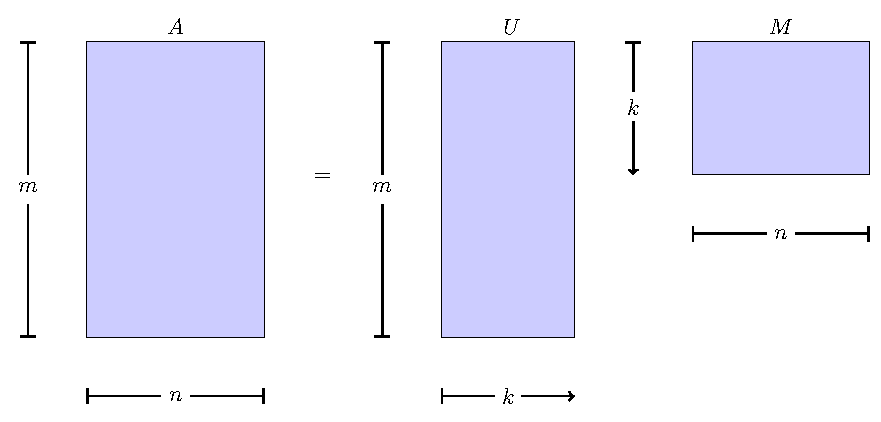
\includegraphics[width=1\textwidth]{ALS_FIG.pdf}

\caption{ALS Decomposition}
\label{fig:ALS Decomposition}
\end{figure}


Let us consider the first row of $R$, which will have all the ratings
given by the fist user. Let us assume the user has seen movies 1, 213, 315,
1744, 2133, 7044, 9012, 12344 and 16890  so in a total of 9 movies. Forming a
vector of the known ratings for the first user we have $\begin{bmatrix}
                                          1 & 213 & 315 & 1744 & 2133 & 7044 &
9012 & 12344 & 16890                                    
                                          \end{bmatrix}
$, let
this be denoted by $b$. We initialize the $M$ matrix in a particular way, and as
shown in the Figure 2.1 it has $n_m$ rows and $n_f$ columns. The matrix $U$ has
$n_u$ rows and $n_f$ columns. For the case of the first user we can form a
sub-matrix of $M$, denote this by $M_u$. This matrix $M_u$ will have all the
rows from $M$ corresponding to the movies seen by the user $u$, the first user
in this case. Let $\boldmath{u}$ be the row vector from $U$ corresponding to the
considered user, .i.e, first user. Now we have three components $R(1,:)$, the
row vector having the nine ratings of the nine movies seen by user 1, $u_1$ the
unknown first row of $U$ matrix, $M_u$, a submatrix of $M$ consisting of the
rows corresponding to the movies rated by the user 1. Figure 2.2 shows the
symbolic representation of this single ordinary least squares problem
formulation, $ \|{M_uu-R(1,:)}\|$. This is done for all the users to obtain the
$U$ matrix. Next this $U$ matrix is used to estimate the new $M$ matrix. The $U$
and $M$ are estimated alternatively until some convergence criteria is
satisfied. 


\begin{figure}[h!]

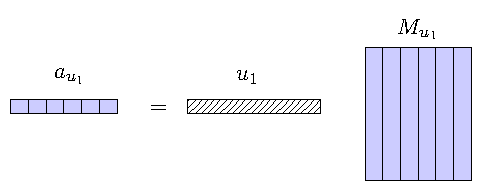
\includegraphics[width=0.6\textwidth]{ALS_FIG2.pdf}
\caption{OLS }
\label{fig:OLS Decomposition}
\end{figure}










\chapter{Temporal Dynamics\index{Temporal Dynamics}}



\textsf{ In this chapter we explain all the aspects related to Temporal Dynamics
in the NETFLIX data. We also show how to build temporal bias based model.}

\section{Temporal Dynamics in NETFLIX data}
The main goal in this work is to integrate temporal information into the
Recommender System model we are building based on collaborative filtering. It is
very important to consider temporal dynamics since the vast amounts of data we
are flooded with is dynamic in nature, and most of the information retrieval
tools today consider only the snapshot of this data, thereby loosing one very
potential dimension. In this chapter we present in detail the significance of
temporal dynamics in general and with respect to NETFLIX and also how to include
temporal dynamics into the model. \\


Since we are trying to improve the prediction rate by including temporal
effects, it is very critical to identify and uncover all possible temporal
effects within the NETFLIX data. This section summarizes and reports the
temporal analysis of the NETFLIX data.

\section{Tracking Drifting Customer Preferences}
The phenomena of $Concept drift$ is evident in the case of NETFLIX system, as we
can see that the user preferences of movies keep changing over time due to
various reasons. Concept drift means when the statistical properties of the
target variables change with time, like how user preferences change with new
release of new movies. In our case where we are trying to collaborate using
interconnected preferences among users, it is a challenge since each of the
interacting users could be drifting in different ways and also they are in
different time instances. There are mainly three kinds of approaches to include
time apect, \emph{instance selection}, in which only the recent instances are
considered, discarding off other instances. All instances within a specific time
period is given equal opportunities discarding instances ouside this period.
This obviously leads to lose of information.  In 2005, a time-weighted CF method
was proposed by Ding and Li in \cite{Ding:2005:TWC:1099554.1099689}, in
which depending on how recent the ratings are they are weighted accordingly,
these models do include time but only as weighted schemes, this is the second
approach called \emph{instance weighting}. The third approach is the
\emph{ensemble learning}, in which predictions from number of models are
combined to give a final prediction. But in this approach, if each of the
individual predoctors capture local behaviour, the global patterns are
overlooked.  A more complex approach was proposed by Koren et al, in
\cite{Koren:2010:CFT:1721654.1721677}, in
which the various complex time parameters are incorporated into the model.
We have built our model based on the following guidelines, \\
\begin{itemize}
  \item We try to model for the entire time period, instead of any particular
instances or particular time periods.
  \item We try to capture the multiple drifts based on the user, both sudden
changes and gradual changes.
  \item All the various drifts will be combined into a single framework.
\end{itemize}

\begin{example}
 As an example consider two users Joe(21 years old) and John(41 years old)
rating a common movie Godfather(1972). During November 2008, Godfather was voted
No. 1 in Empire magazine's list of The 500 Greatest Movies of All Time. Joe
after seeing this watched the movie and gave his rating. On the other hand John
had rated the movie 20 years back. This makes them both roughly the same age
when they have rated the movie, however in a different time instance. It is
clear that Joes rating could have had certain bias caused by $classical$ nature
of the movie.
\end{example}

\section{Temporal Dynamics in NETFLIX Data}
Here we would show through plots the dynamic nature inherent in the data with
respect to time. 


\begin{figure}[h]
\centering
\subfigure[Movie Means by Date]{
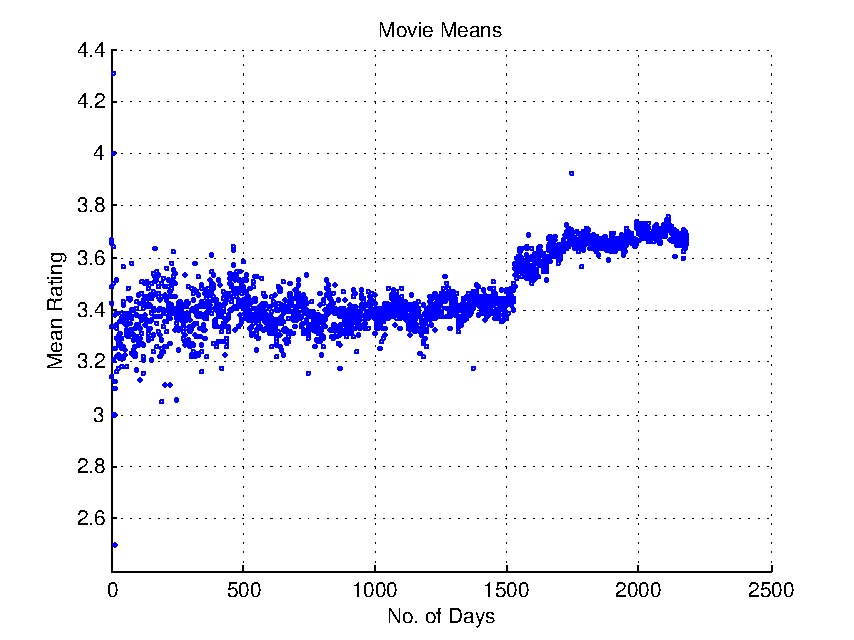
\includegraphics[width=0.45\textwidth]{./New/MovieMeans_AllMovie.pdf}
\label{fig:MovMean}
}
\subfigure[Movie Means by Movie Age]{
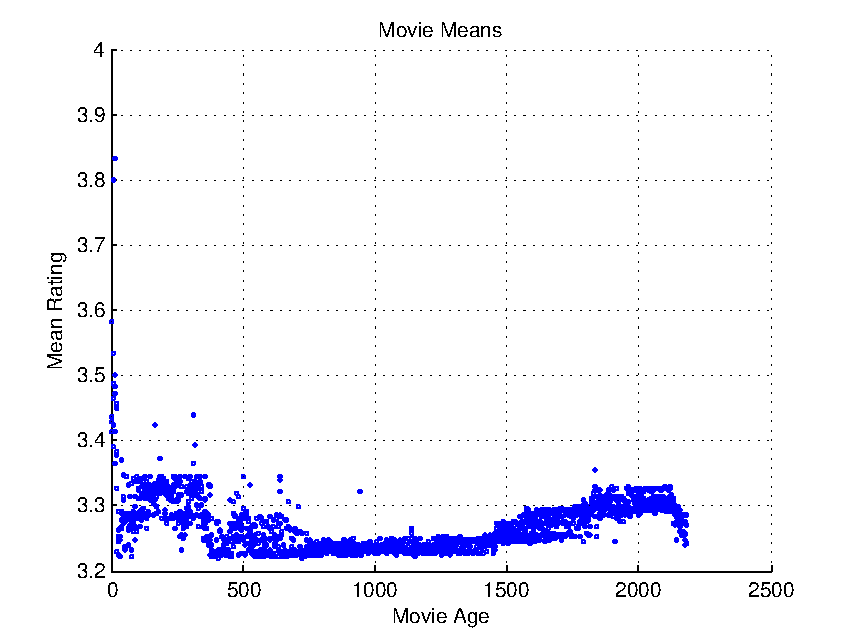
\includegraphics[width=0.45\textwidth]{./New/MovieMeans_AllMovie_Age.pdf}
\label{fig:MovMean_Age}
}\\

\label{fig:MovieMean_temporal}
\caption{Movie Means vs Time}
\end{figure}



\section{Temporal-Factor Model}
As we had seen in the previous chapter, that all the non user-item interaction
effects are encapsulated in the \emph{Baseline predictors}, we will show here
who we intend to include temporal baseline predictors. Here we explain the
theoretical analyses and findings related to various time changing aspects of
users and of movies. It is clear that the time dynamics of movies will be more
gradual than that of the users. The movies are analysed based on a large number
of users who have rated the single movie, but however as an individual user the
temporal analyses is done on large number of unrelated factors, hence the user
behaviour seems more complex and less uniform compared to the movies. \\
The main challenge is to parameterize the user-drift and the movie-drift as
appropriately as possible. The first and foremost consideration is how
transitory are the user-drift and the movie-drift. As we will expalin in detail
the movie-drift seems to be more uniform and less transient than the user-drift,
hence it is wise to consider finer time resolution to model user-drift and
coarser resolution for movies. The final model should however account for both
temporal effects spanning on a longer duration and the more transitory changes. 
For example, movies dont change on a daily basis, some of the factors which
could affect the movies dont occur often like appearance of an actor in another
movie, or the movie winning an award or the movie recieving appreciation from a
critique. On the contrary consider an user, who usually rates relative to other
ratings, so his rating scale could vary everytime he has seen on influencing
movie proir to the current movie of interest. A user who usually rate 4 for
average movies, could be influenced to rate the same kind of average movies by
3. \\

\begin{figure}[h!]
\centering
\subfigure[Monthly Average of All movies]{
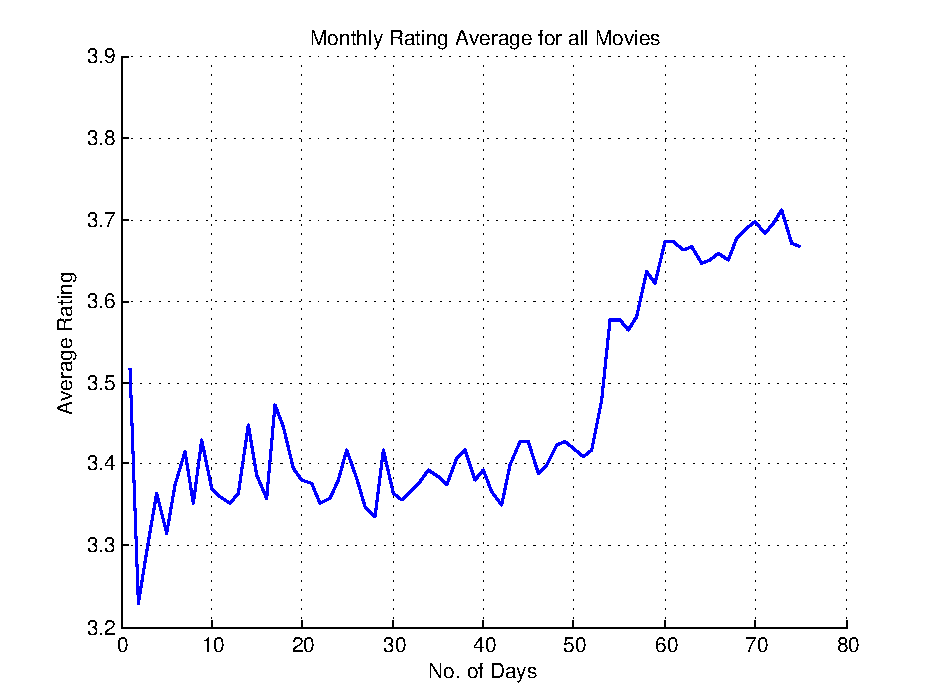
\includegraphics[width=0.45\textwidth]{./New/MonthlyAve_AllMovies.pdf}
\label{fig:MonthlyAllMov}
}
\subfigure[Weekly Average of all movies]{
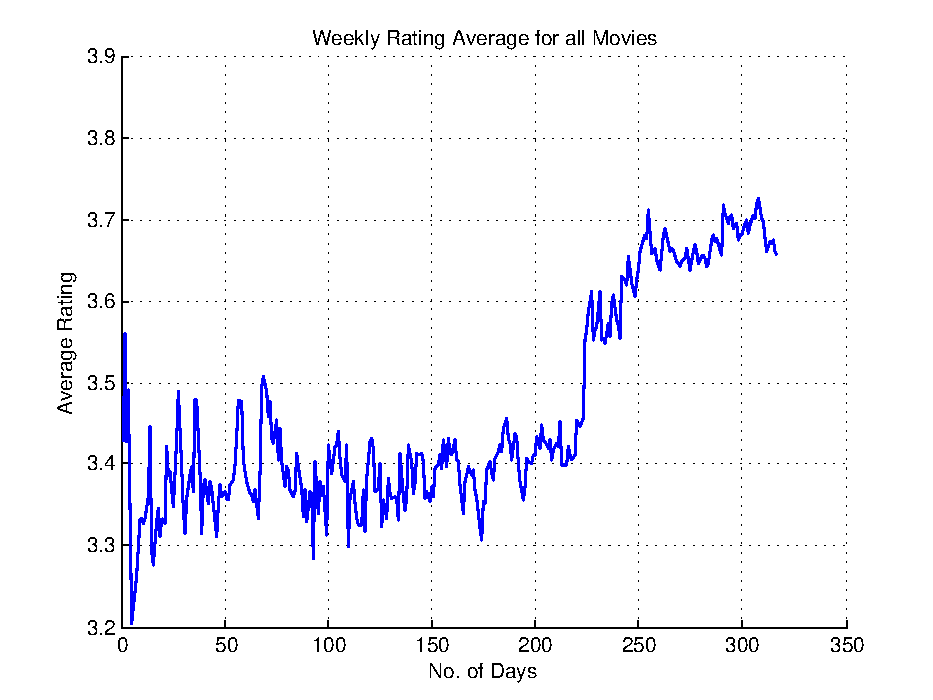
\includegraphics[width=0.45\textwidth]{./New/WeeklyAve_AllMovies.pdf}
\label{fig:WeeklyAllMov}
}\\

\subfigure[Monthly Average of movie 129]{
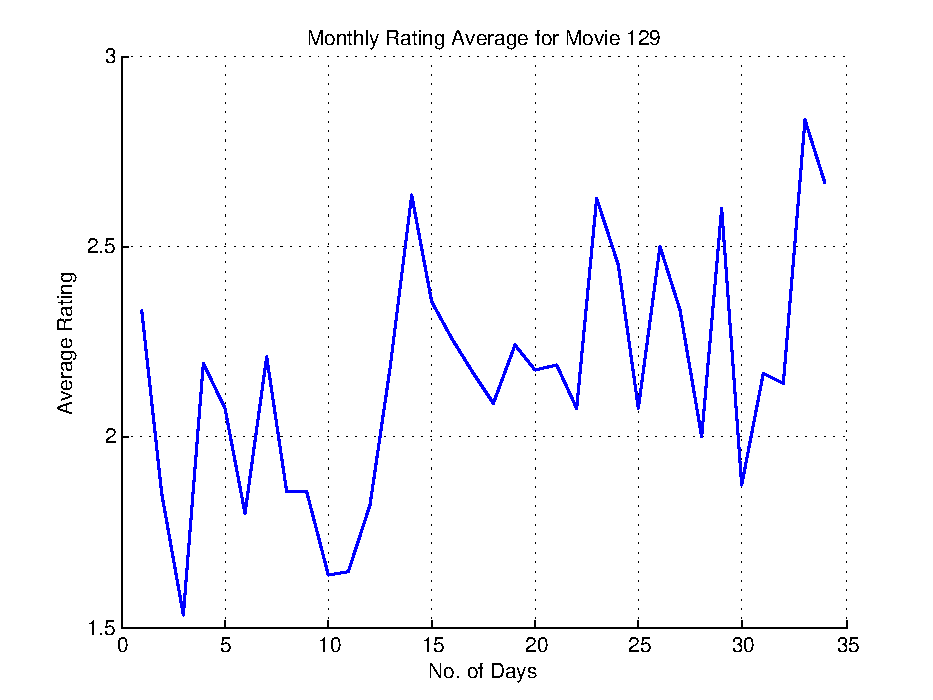
\includegraphics[width=0.45\textwidth]{./New/MonthlyAve_M129.pdf}
\label{fig:MonthlyM129}
}
\subfigure[Weekly Average of movie 129]{
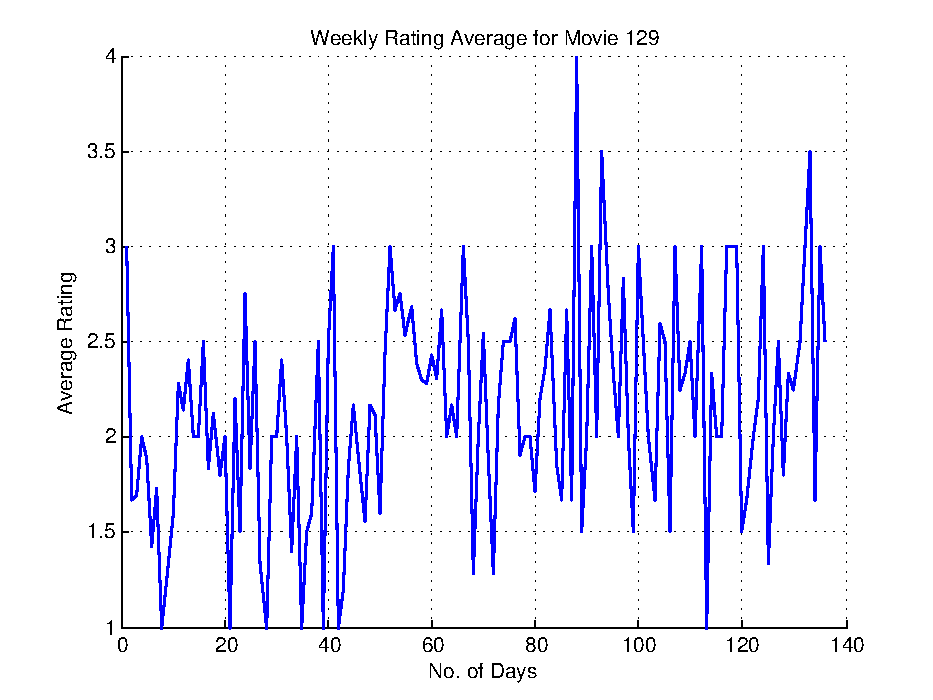
\includegraphics[width=0.45\textwidth]{./New/WeeklyAve_M129.pdf}
\label{fig:WeeklyM1476}
}\\

\subfigure[Monthly Average of movie 1476]{
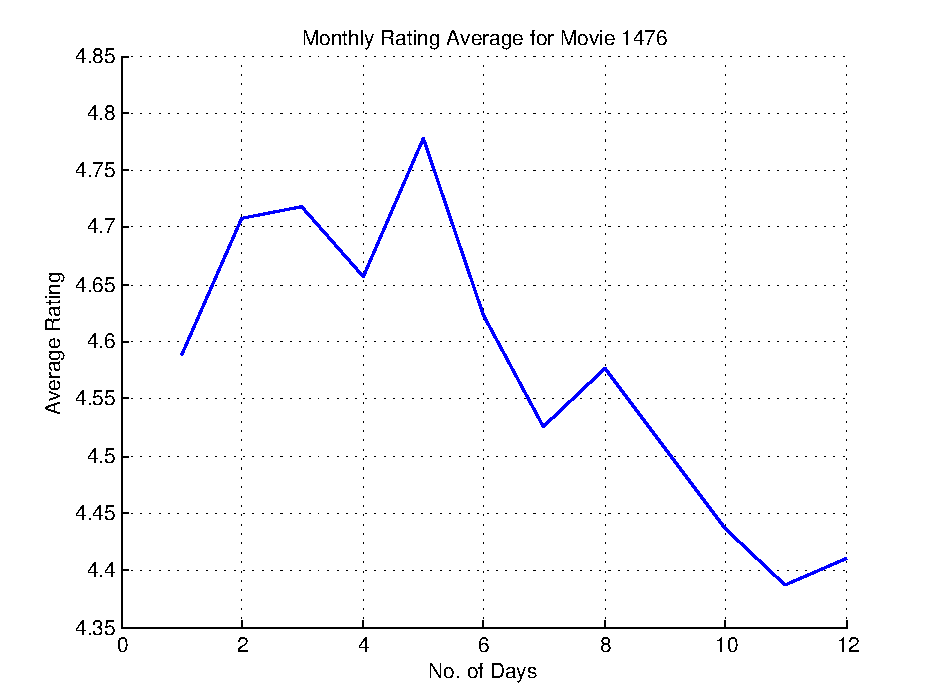
\includegraphics[width=0.45\textwidth]{./New/MonthlyAve_M1476.pdf}
\label{fig:MonthlyM129}
}
\subfigure[Weekly Average of movie 1476]{
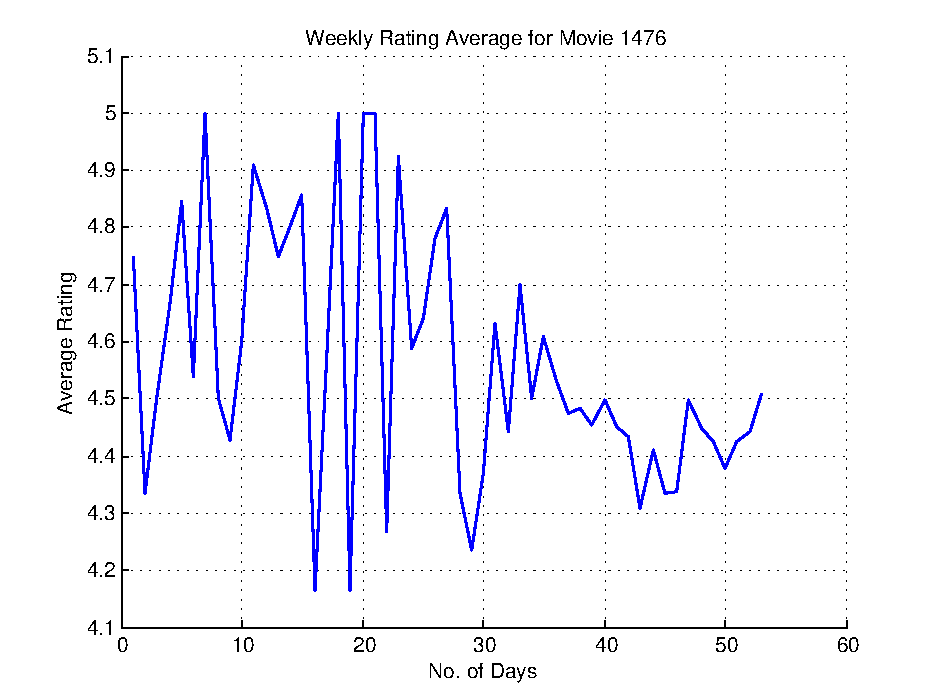
\includegraphics[width=0.45\textwidth]{./New/WeeklyAve_M1476.pdf}
\label{fig:WeeklyM1476}
}\\

\label{fig:MonthlyWeeklyAverages}
\caption{Monthly and Weekly Averages}
\end{figure}

We begun by experimenting for different time periods called \emph{bins} in order
to catch the movie-drifts.  The whole time period spans over 300 weeks, and
after several rounds of testing a 10 week period was chosen as the optimal bin
length. Hence a total of 30 bins suffice to span the entire data. With each bin
we associate it with a bias(transient part), which is simply the difference
between the overall movie mean and the mean of the movie for that bin period.
Interpolation is done for bins where there are no ratings. Each rating instance
of a movie in the training data is associated with a bin value between 1 and 30.
Hence the movie bias would have two components a stationary part, $b_{i}$ and a
transient part $b_{i,Bin(t)}$ \refname{[7]}. \\

\begin{equation} 
 b_{i}(t)=b_{i}+b_{i,Bin(t)}
\end{equation}

We have in this thesis work considered only movie related temporal dynamics,
however we would comment on a possible approach to capture temporal dynamics
related to the more complicated user bias. In case users we need to parameterize
for both long term and short term changes. A simple linear function could be
used to capture the gradual user-bias drift. Each user will have an average
rating date, and for every rating instances of this user the deviation could be
a function of the difference of the dates. Regarding sudden drifts, we need to
capture the drift on daily basis. The minimum step length could be larger than a
day also. In the NETFLIX data the user on an average rates on 40 different days,
hence we need 40 different paramaters for every user on an average. These two
factors could model the temporal dynamics of the users.  




\chapter{Mathematical Background\index{Mathematical Background}}

\textsf{ In this chapter we provide the mathematical proofs which form the basis
of the prediction models. The main concept of matrix factorization is explained
mathematically. Singular value decomposition is explained in detail, and some
issues regarding the disadvantages in the present scenario is explained. An
substitute method Alternate Least Squares is explained. And lastly low rank
approximation is explained.}

\section{Introduction to Matrix Factorization}
Since this chapter is dedicated to the mathematical principles that drives the
prediction models, we can begin with a direct statement, the data matrix is
factorized into simpler matrices which are constrained on its dimensionality.
Different types of constraints can be imposed on the factorization, but for the
particular machine learning task of collaborative filtering we have only used
the low rank approximation. Collaborative filtering can be considered as
\emph{matrix completion} problem, where we are trying to fill in the missing
entries of the sparsely filled rating matrix $R$ $\in\mathbb{R}^{u,i}$. We
complete the rating matrix by approximating it to a full matrix $\hat{R}=PQ'$,
where $P \in\mathbb{R}^{u,k}$ and $Q \in\mathbb{R}^{i,k}$. 

$P$ and $Q$ are unconstranied \emph{factor matrices} and we will show that if
$\hat{R}$ is the best approximation of the original rating matrix, then the
\emph{rank} of $\hat{R}$ is at most $k$. 

Now that we have had a fair idea of how to approach the problem, the next
important concern is to decide in what sense do we want to approximate the data
matrix, or how do we measure the discrepency between the original matrix and the
approximated matrix. The simplest way would be to measure the \emph{Frobenius
distance} between the two,
\[
 \|{R-\hat{R}}\|_{F}^2 = \sum_{ui}^{}(R_{ui}-\hat{R}_{ui})^2
\]
But we use the Root Mean Squared Error(RMSE) to measure the accuracy. 

There might also be a necessity in applicatons like clustering to impose a
constraint on the factored matrices other than only on rank of approximating
matrix. Since clustering is based on some kind of distance measure and distance
can never be negative, it is obvious that we need to impose a non-negative
constraint on the factored matrices. In such cases we cannot rely on SVD as it
can generate negative elements. Instead we might want to compute the rank-$k$
approximation in the following way \cite{eld-mm:07}, \\
\[
  A\approx WH,		W,H\geq0
\] \\

\section{Matrix approximation using SVD}
\begin{theorem}[SVD]
 Any $m \times n$ matrix A with rank k, with $m \geq n$, can be factorized \\
\begin{equation}
  A = U\begin{pmatrix}\Sigma\\0\end{pmatrix}V^{T},
\end{equation}
where $U \in \mathbb{R}^{m \times m}$ and $V \in \mathbb{R}^{n \times n}$, and
$\Sigma \in \mathbb{R}^{m \times n}$ is a diagonal matrix, i.e., $\Sigma =
diag(\sigma_1,\sigma_2,...\sigma_n)$, with $\sigma_1 \geq \sigma_2 \geq ... \geq
\sigma_n \geq 0$. Here $\sigma_1,...,\sigma_n$ are called singular values of A.
The column vectors of U and V are called the right and left singular vectors of
A, respectivley.  
\end{theorem}
The matrix A can be constructed from the singular values as shown below, \\
\begin{equation}
 A=\sum_{i=1}^{n}\sigma_i u_i v_i^T
\end{equation}
The matrix $U$ can be written as $U=[U_1 U_2]$, where $U_1 \in \mathbb{R}^{m
\times n}$. We can obtain the matrix $A$ by the \emph{outer} \emph{product}
\emph{form} in a thin version as shown below,
\[
 A=U_1 \Sigma V^T = \begin{pmatrix}u_1&u_2&\cdots&u_n\end{pmatrix}
  \begin{pmatrix}
  \sigma_1 &         &        &        \\
           & \sigma_2&        &        \\
           &         & \ddots &        \\
           &         &        & \sigma_n
 \end{pmatrix}
 \begin{pmatrix}v_1^T\\v_2^T\\\vdots\\v_n^T\end{pmatrix}\\
\] \\
Now moving ahead with matrix approximation, let us consider our original matrix
$A$, as sum of a low-rank matrix and a small noise, $A_0 + N$. Since it is an
approximation problem we will try to minimise the noise $N$, by estimating the
\emph{correct rank} of $A_0$, this rank is known as \emph{numerical rank}.
\cite{eld-mm:07}. Now the approximation looks like this, \\
\[
 A = \sum_{i=1}^{n}\sigma_i u_i v_i^T \approx \sum_{i=1}^{k}\sigma_k u_k v_k^T
\]\\
\begin{theorem}[Eckart-Young theorem]
 For a matrix A $\in \mathbb{R}^{m \times n}$, with $rank(A)=r>k$. The Frobenius
norm of the matrix approximation problem \\
\begin{equation}
 \min_{rank(\hat{A})=k}\|{A-\hat{A}}\|
\end{equation}\\
which has the solution of 
\begin{equation}
 \hat{A}=U_k \Sigma_{k} V_k^T,
\end{equation}\\
where $U_k = \begin{pmatrix}u_1&u_2&\cdots&u_k\end{pmatrix}$, $V_k=
\begin{pmatrix}v_1^T\\v_2^T\\\vdots\\v_n^T\end{pmatrix}$ and
$\Sigma_k=diag(\sigma_1,\sigma_2,...,\sigma_k)$. Equation 4.3 has the minimum
solution of
\begin{equation}
 \|{A-\hat{A}}\|_{F}=\left(\sum_{i=k+1}^{p}\sigma_i^2\right)^{1/2},
\end{equation}
where $p=min(m,n)$.
\end{theorem}

\section{Matrix approximation using Alternating Least Squares}
\subsection{Disadvantage of SVD}
In this thesis work we have done the implementation using MATLAB, and we use the
function $[U,S,V]=svds(A,k)$ to obtain the singular value decomposition of a
sparse matrix $A$ of rank $k$. However elegant is the method of $SVD$, it
unfortunately fails to produce good predictions. The $SVD$ approximates a rating
matrix by minimizing the \emph{Frobenius norm} of $|R-\hat{R}|$. This is
equvivalent to minimizing the RMSE between individual elements in the rating
matrix. Since the majority of the elements are \emph{unknowns}, and it is our
belief that MATLAB while calulating \emph{SVD} considers these \emph{unknowns}
as zeros, whereas these are not zeros and hence this approach is flawed.
In the Appendix A, we give a detailed explanation as to why SVD is not
appropriate to find the low-rank matrix approximation in our case, where our
data matrix is very sparse($1\%$-dense). 

\subsection{Problem formulation w.r.t ALS}

This approach is based on the article \cite{Zhou:2008:LPC:1424237.1424269}.
Let $U=[\bold{u_i}]$ be the user feature matrix where $\bold{u_i} \subseteq
\mathbb{R}^{n_f}$ and $i=1,2,...,n_u$, and let $M=\bold{m_j}$ be the item or
movie feature matrix, where $\bold{m_j} \subseteq
\mathbb{R}^{n_f}$ and $j=1,2,...,n_m$. Here $n_f$ is the number of factors,
i.e., the reduced dimension or the lower rank, which is determined by cross
validation. The predictions can be calculated for any user-movie combination
$(i,j)$, as $r_{ij}=\bold{u_i} \cdotp \bold{m_j}, \forall i,j$. Here we minimize
the loss function of $U$ and $M$ as the condition in the iterative process of
obtaining these matrices. Let us start by considering the loss due to a single
prediction in terms of sqaured error: 
\begin{equation}
 \mathcal{L}^2(r,\bold{u},\bold{m})=(r-<\bold{u},\bold{m}>)^2.
\end{equation}

Based on the above equation generalizing it for the whole data set, the
\emph{empirical} total loss as:
\begin{equation}
 \mathcal{L}^{emp}(R,U,M)=\frac{1}{n} \sum_{(i,j) \in
I}\mathcal{L}^2(r_{ij},\bold{u_i},\bold{m_j}),
\end{equation}
where $I$ is the known ratings dataset having $n$ ratings. 

Based on the above, we can formulate our low rank matrix approximation problem
as 
\begin{equation}
(U,M)=arg \min_{(U,M)}\mathcal{L}^{emp}(R,U,M).
\end{equation}

Here the number of elements or free parameters we need to determine is $(n_u +
n_m)n_f$, but in our initial known data matrix, .i.e, $R$ we only have $1\%$ of
$n_un_m$ elements. While solving Eq. (4.8) with a sparse $R$ matrix leads to
overfitting. To avoid this we use Tikhonov regularization, our emperical loss
term get another term as shown below:
\begin{equation}
 \mathcal{L}_{\lambda}^{reg}=\mathcal{L}^{emp}(R,U,
M)+\lambda(\|U\Gamma_U\|^2+\|M\Gamma_M\|^2),
\end{equation}
where $\Gamma_U$ and $\Gamma_M$ are Tikhonov matrices. In the next section we
will discuss in detail about how to form these Tikhonov matrices.
\subsection{Regularized ALS}

According to the article \cite{Zhou:2008:LPC:1424237.1424269}, it is best to use
weighted-$\lambda$-regularization, which is as shown below:
\begin{equation}
 f(U,M)= \sum_{(i,j) \in I}(r_{ij}-\bold{u}_i^T\bold{m}_j)^2+\lambda(\sum_i
n_{u_{i}}\|\bold{u}_i\|^2+\sum_j n_{m_{j}}\|\bold{m}_j\|^2),
\end{equation}
The above equation can is somewhat an vectorized version of Eq. (4.9), where the
Tikhonov matrices are replaced by $n_{u_{i}}$ and $n_{m_{j}}$, which are nothing
but the number of ratings of user $i$ and movie $j$. Below equations show how
these terms are related to Tikhonov matrices:
$$\Gamma_U=diag(n_{u_{i}})		\Gamma_M=diag(n_{m_{j}})$$
Now we will discuss how to solve for matrices $U$ and $M$, this is the
mathematical explanation of what was explained under Temporal Bias + ALS model
in Sec. (2.3.3). The matrix $U$ is approximated column wise, i.e., $u_i$, is
determined by solving the regularized least squares problem, using the known
ratings vector of user $i$ and the feature vectors $m_j$, which are the columns
of $M$ matrix corresponding to the movies seen by the user $i$. Let us
represent 
Eq. (4.10), is a simple differential equation style as follows:
\begin{equation}
 f(u,m)=(r-um)^2+\lambda(nu^2+nm^2)
\end{equation}
to minimize this function we equate the first partial differential w.r.t $u$ of
the function $f$ to $0$.
\begin{align}
& \frac{1}{2} \frac{\partial f}{\partial u_{ki}} = 0, & \forall i,k \\
 \implies & \sum_{j\in I_i}(\bold{u}_i^T\bold{m}_j-r_{ij})m_{kj}+\lambds
n_{u_{i}}u_{ki}=0, & \forall i,k \\
 \implies & \sum_{j\in I_i}m_kj\bold{m}_j^T\bold{u}_i
+\lambda n_{u_{i}}u_ki = \sum_{j\in I_i}m_{kj}r_{ij}, & \forall i,k \\
\implies & (M_{I_{i}}M_{I_{i}^T}+\lambda
n_{u_{i}}E)\bold{u}_i=M_{I_{i}}R^T(i,I_i), & \forall i,k \\
\implies & \bold{u}_i = A_{i}^{-1}V_i, & \forall i \\
  \end{align}

where $E$ is $n_f \times n_f$ identity matrix, $V_i=M_{I_{i}}R^T(i,I_i)$ and
$A_i=M_{I_{i}}M_{I_{i}}^T+\lambda n_{u_{i}}E.$ 

Now in the same way by starting with a known $U$ matrix, the movie feature
matrix $M$ is approximated by computing the individual column vectors of $M$ as
shown below: \\
\begin{align*}
 & \bold{m}_j=A_{j}^{-1}V_j, & \forall j,
\end{align*}
where $A_j=U_{I_{i}}U_{I_{i}}^T+\lambda n_{m_{j}}E$ and $V_j=U_{I_{i}}R(I_j,j)$.
$U_{I_{i}}$ is the sub-matrix of $U$, where only $i \in I_j$ are selected.
$R(I_j,j)$ is the column vector which is obtained from the rating matrix $R$, by
selecting all the elements from column $j$ and rows corresponding to $i \in I_j$

\section{Evaluation Metrics}
With the advent of the NETFLIX Competition, \emph{accuracy} has become one of
the most important defining properties of Recommender systems. Hence it is
worthwhile to discuss about different methods of measuring accuracy. The choice
of metrics for accuracy might depend on the kind of systems under study, like if
it is \emph{rating prediction system} or \emph{decision support system}. For the
former we can use statistical accuracy measures where we compare the predicted
value with known actual values, for example the \emph{MAE(Mean Absolute Error)},
\emph{RMSE}, \emph{Correlation} etc. In the case of decision support systems,
where it is required to produce a list of high-relevance items, like in the
\emph{top-N} recommendation systems, the metrics used to measure accuracy are
\emph{precision}, \emph{recall}, or \emph{F-measure} etc. 

\subsection{Mean Average Error}
Let us consider, $\mathcal{T} = \{r_{ij} \exists \mbox{ in } Q_{\text{test}}
\mid \mbox{user } i
\in \mathcal{U} \mbox{ have rated movie } j \in \mathcal{M} \}$, to be the test
set. Then the MAE can be defined as,
\begin{equation}
 MAE = \sum_{r_{i,j}\in{\mathcal{T}}}\frac{|\hat{r}_{ij}-r_{ij}|}{|T|}
\end{equation}
where $\hat{r}_{ij}$ is the predicted rating and $r_{ij}$ is the actual rating,
and $|T|$ is the size of the test set. The goal is to minimize this value to get
better accuracy.

\subsection{RMSE}
For the same test set as shown above, the RMSE is defined as, 
\begin{equation}
  RMSE =\left(
\frac{\sum_{r_{i,j}\in{\mathcal{T}}}{(\hat{r}_{ij}-r_{ij})^2}}{|T|}\right)^{1/2}
\end{equation}

\subsection{Correlation}
If we consider the predicted and the known values to be vectors, then the
correlation gives the proximity of the two vectors. \emph{Pearson Correlation
Coefficient} is an example, which is defined by
\begin{equation}
 \rho_{\hat{r},r}=\frac{cov(\hat{r},r)}{\sigma_{\hat{r}}\sigma_r}
\end{equation}
Higher the value better the accuracy in this case. Geometrically this can be
viewed as the \emph{cosine} of the angle between the two vectors. 

\subsection{Precision and Recall}
In the general \emph{Information retireval} point of view, the precision is
defined as,
\begin{equation}
 P=\frac{D_r}{D_t}
\end{equation}
where $D_r$ is the number of relevant documents retrieved and $D_t$ is the total
number of documents retrieved \cite{eld-mm:07}. But in the
Recommender system point of view the documents are replaced by items, and the
user interest according to the user profile is used instead of the explicit
query. 

Recall is defined as,
\begin{equation}
 R=\frac{D_r}{N_r}
\end{equation}
where $N_r$ is the total number of relevant documents in the database, which in
the case of recommender systems would be the total number of items in the whole
data.

\subsection{F-Measure}
This is a way to combine the precision and recall into one metric, a simple F-1
measure is the harmonic mean of precision and recall. 













\chapter{Results\index{Results}}


\textsf{In this chapter we present the results of the epxeriments conducted,
reasoning the motivation towards the built models. We also talk about aspects
which were considered but not implemented.}

\section{Overview of Different Models}
The principles behind designing the model are firstly, to accurately account for
biases of various types and secondly, formulation of an efficient low-rank
matrix approximation method. The first principle involves identifying different
biases, like, the user-bias, movie-bias and temporal biases w.r.t users and
movies. These biases are the non-interacting parts between the users and movies,
and they are encapsulated into the baseline predictor. These values are
initially subtracted from all the known ratings. They will be integrated back
into the factor model for the new predicted ratings. We have experimented with
three types of biasing techniques, first without any bias, second, with only
static bias, and third, with temporal movie biases. Moving ahead to the
factorization itself, we start with the SVD technique and owing to the
issue of the MATLAB method svds treating the unknown ratings as zeros, we
develop a new factorization technique based on
weighted ALS. Within the ALS algorithm we have two types of initialization
methods, hence leading to ALS-I and ALS-II. The table below shows the various
models built by combining the different biasing and factorizing techniques
mentioned.


\begin{table}
\begin{center}
 
     \begin{tabular}{|c|c|c|c|}
       \hline
        & SVD & ALS-I & ALS-II \\ \hline
       None & Model 1 & Model 6 & Model 7\\        
       $NonTemp_{mu}$ & Model 3 & - & Model 8\\
       $Temp_{mu}$ & Model 2 & - & Model 9\\
       $NonTemp_b$ & - & Model 4 & -\\
       $Temp_b$ & - & Model 5 & -\\ \hline
    \end{tabular}
    \caption{Different Model}     
\end{center}
\end{table}

\subsubsection{SVD}
While using this method, which is [U,S,V]=svds(R,n), where $R$ is the Rating
matrix and $n$ is the rank of the approximating matrix. We test the models for
different values of $n$, the maximum being $n$=200. 

\subsubsection{ALS-I}
This is the type-I ALS method, where the M matrix is initialized by replacing
the assigning the first row with the mean values of the movies, and filling in
random values at the remaining places. 



\begin{enumerate}
 \item Initialize the M matrix, by assigning the means of movies as
the first row entry, and small random numbers in the remaining entries. 
 \item  With this M, solve for U in order to minimize the loss
function.
 \item Now Keep the U matrix from step 2 fixed, and update the M
matrix.
 \item Repeat these iterations until required convergence criteria
is met.
\end{enumerate}


\subsubsection{ALS-II}
This is the type-II ALS method, where the M matrix is initialized by doing an
SVD on the initial rating matrix R, as shown below:

\begingroup
\begin{center}
\begin{align*}
& [U1,S1,V1]=svds(\hat{R},100) \\
& M=S1*V1' 
\end{align*}
\caption{SVD Initialization of M}
\end{center}
\endgroup


\begin{enumerate}
 \item Initialize the M matrix as shown above row entry, and small random
numbers in the remaining
entries. 
 \item With this M, solve for U in order to minimize the loss
function.
 \item Now Keep the U matrix from step 2 fixed, and update
the M matrix.
 \item Repeat these iterations until required convergence
criteria is met.
\end{enumerate}

\subsubsection{$NonTemp_{mu}$}
This is the non-temporal model with the mean of all movies included in it, it is
given by \\
\begin{equation}
 b_{ui}=\mu+b_u+b_i
\end{equation}
where $b_{ui}$ is the baseline predictor, which encapsulates the non-interacting
parts of user-item relationship, $\mu$ is the mean of all movies which is
$3.6043$, $b_u$ and $b_i$ are the observed deviations from the mean. 

\subsubsection{$Temp_{mu}$}
This is the baseline predictor which involves the tie-changing movie biases,
$b_{i,Bin(t)}$.
\begin{equation}
 b_{ui}=\mu+b_u+b_i+b_{i,Bin(t)}
\end{equation}

\subsubsection{$NonTemp_b$}
This is again non-temporal model, but without the all movie mean $\mu$. This
model is only used in conjuction with the ALS-I method, as in this method the
means is already included into the model during the initialization of M.
\begin{equation}
 b_{ui}=b_u+b_i
\end{equation}

\subsubsection{$Temp_b$}
This is the temporal model without the all movie mean $\mu$, again used for
ALS-I but with time-changing movie biases,
\begin{equation}
 b_{ui}=b_u+b_i+b_{i,Bin(t)}
\end{equation}

\section{Results}
\begin{figure}[h!]
\centering
\subfigure[RMSE for Model 1]{
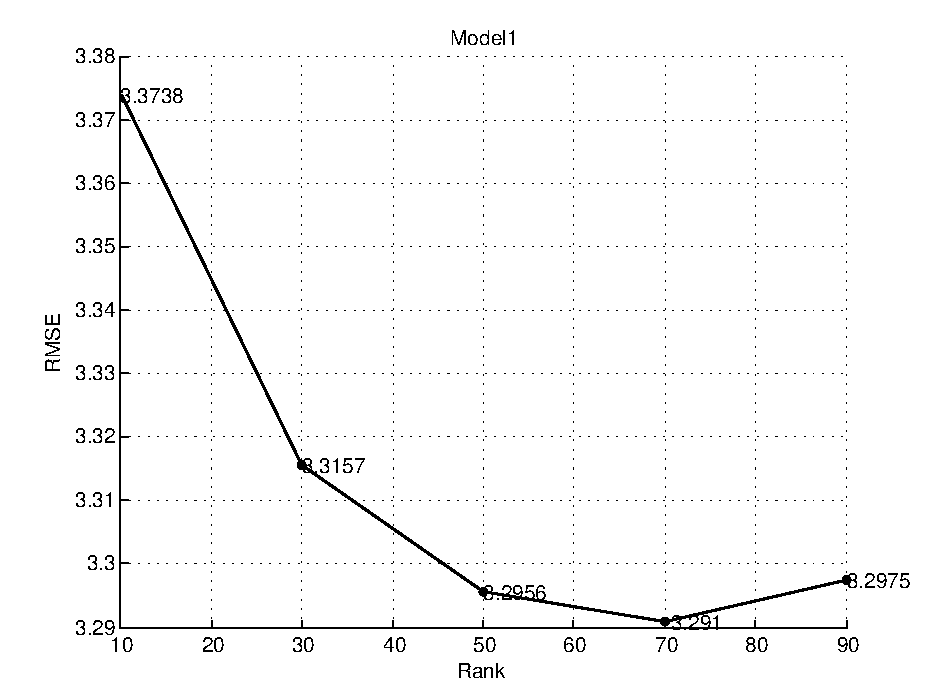
\includegraphics[width=0.45\textwidth]{./Results/plots/model1.pdf}
\label{fig:Model 1}
}
\subfigure[RMSE for Model 2]{
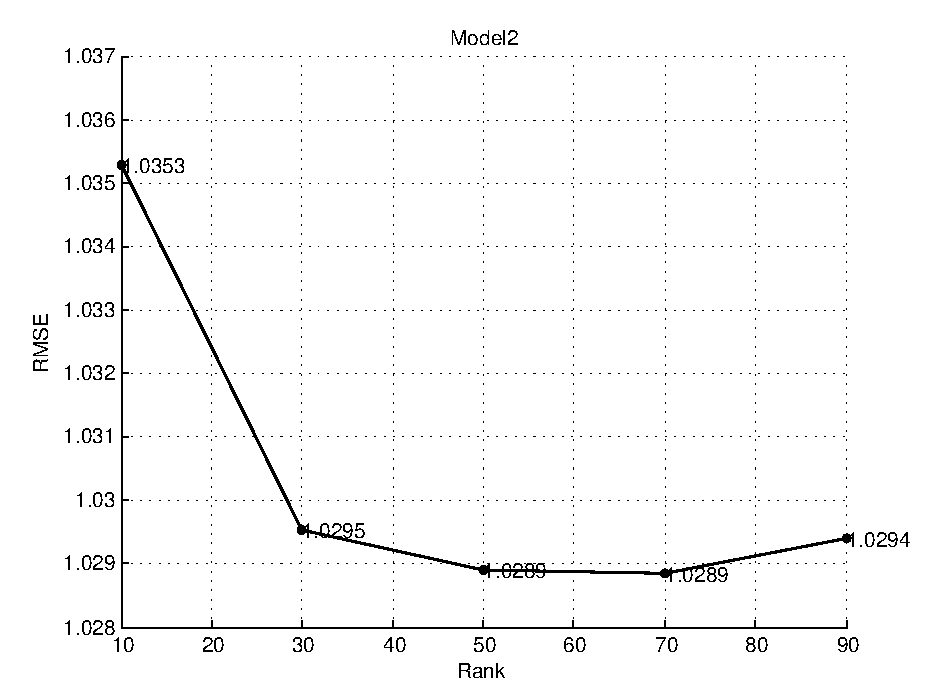
\includegraphics[width=0.45\textwidth]{./Results/plots/model2.pdf}
\label{fig:Model2}
}\\
\subfigure[RMSE for Model 3]{
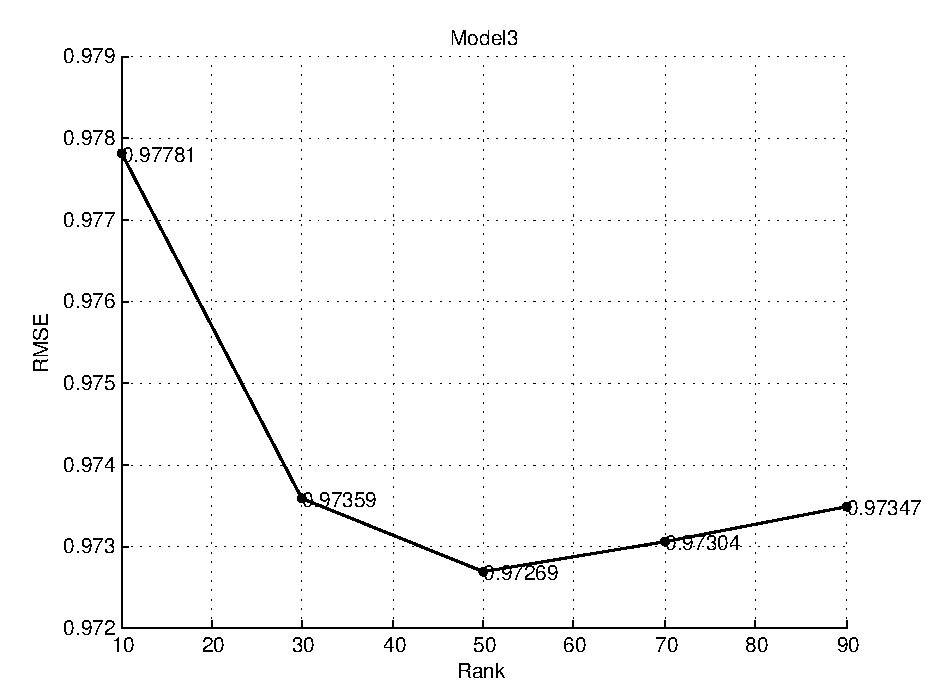
\includegraphics[width=0.45\textwidth]{./Results/plots/model3.pdf}
\label{fig:Model 3}
}
\label{fig:RMSE SVD}
\caption{RMSE: SVD based models}
\end{figure}

In the following figure 5.1, we can see that beyond certain ranks overfitting
occurs. Also we cab observe the improvement in the results by involving the
biases. 

Next we show the results for the ALS based models. Figure 5.2 shows the RMSE of
ALS based models which use the type I initialization technique. 


\begin{figure}[h!]
\centering
\subfigure[RMSE for Model 4 for 30 iterations $N_f=200$]{
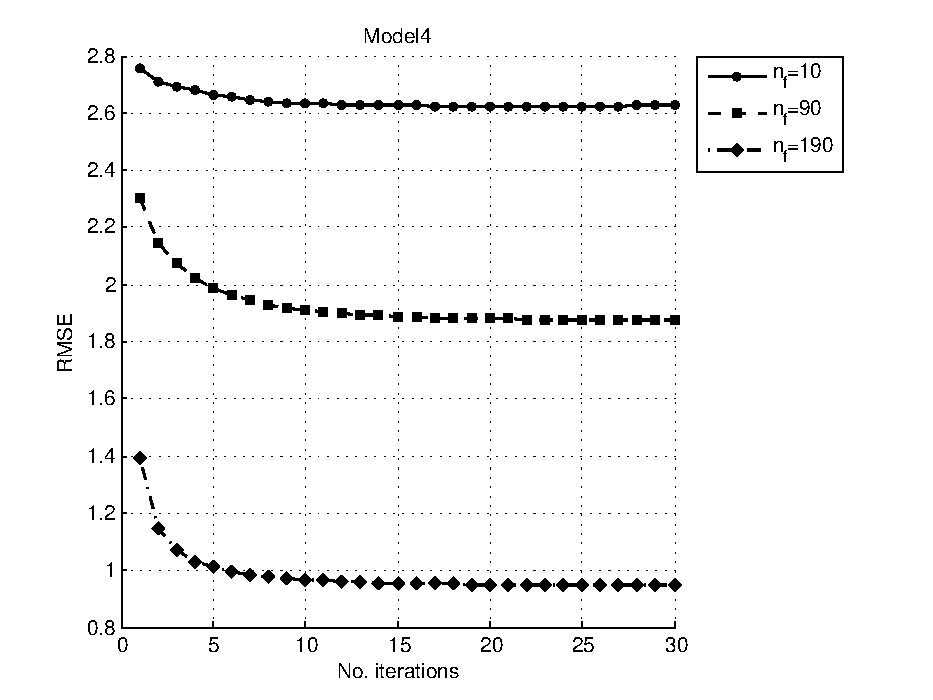
\includegraphics[width=0.45\textwidth]{./Results/plots/model4.pdf}
\label{fig:Model 1}
}
\subfigure[RMSE for Model 4 ]{
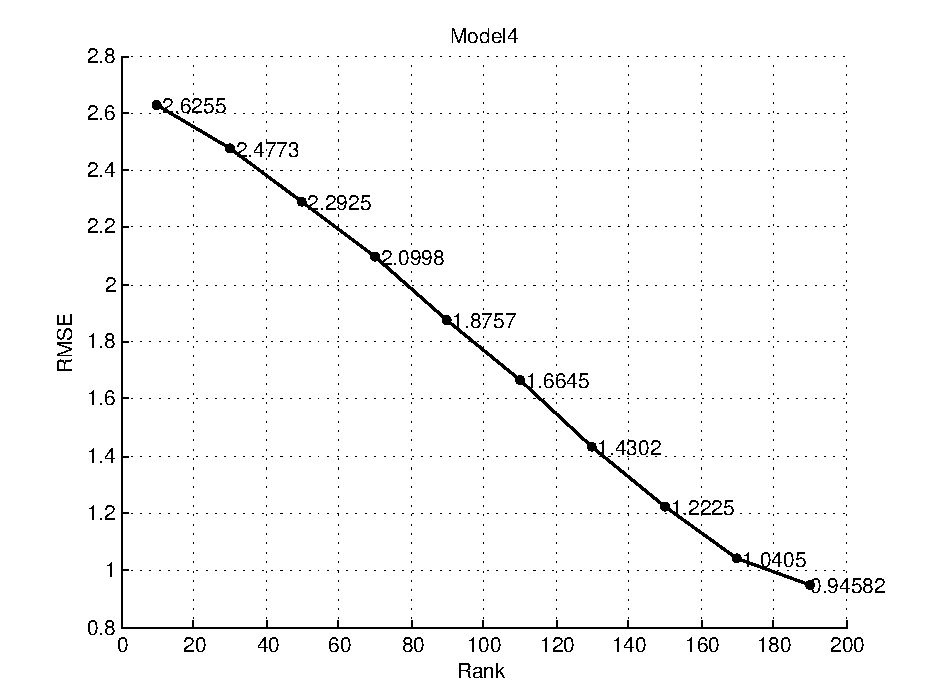
\includegraphics[width=0.45\textwidth]{./Results/plots/model4_1.pdf}
\label{fig:Model2}
}\\
\subfigure[RMSE for Model 5 for 30 iterations $N_f=200$]{
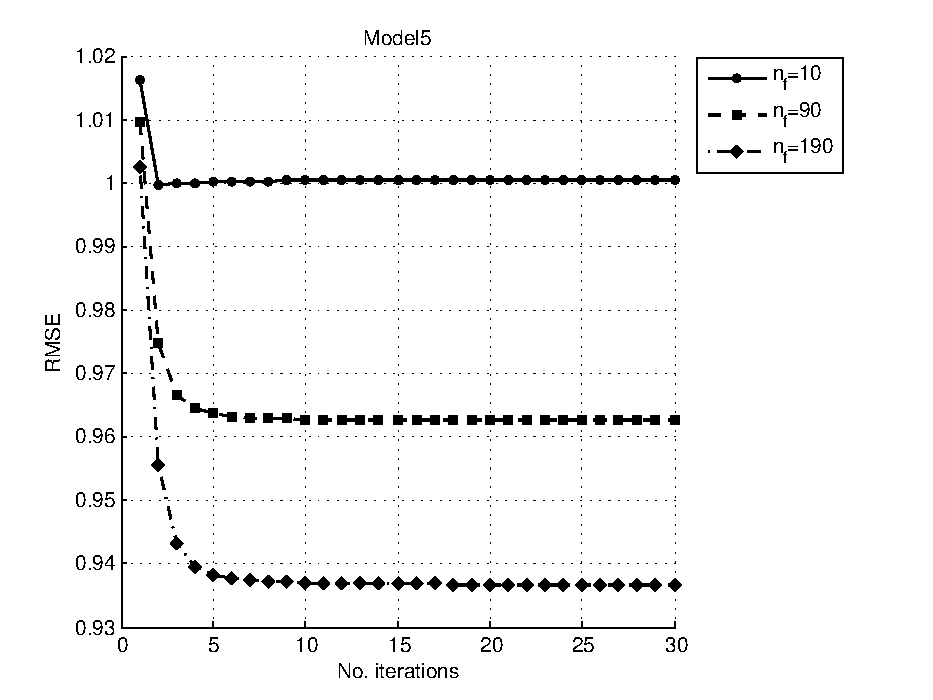
\includegraphics[width=0.45\textwidth]{./Results/plots/model5.pdf}
\label{fig:Model 1}
}
\subfigure[RMSE for Model 5 ]{
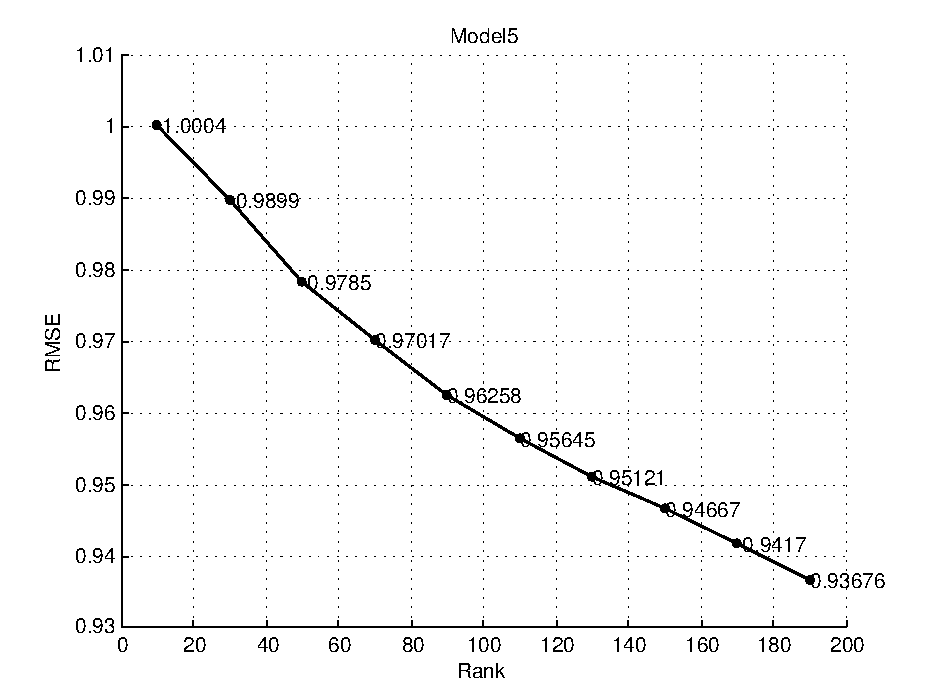
\includegraphics[width=0.45\textwidth]{./Results/plots/model5_1.pdf}
\label{fig:Model2}
}\\
\subfigure[RMSE for Model 6 for 30 iterations $N_f=200$]{
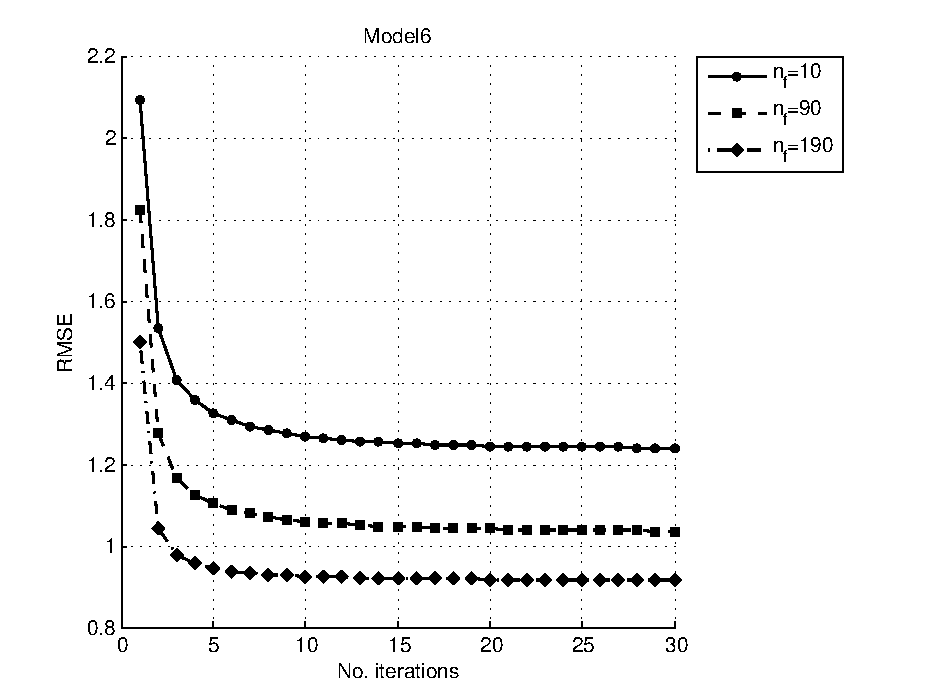
\includegraphics[width=0.45\textwidth]{./Results/plots/model6.pdf}
\label{fig:Model 1}
}
\subfigure[RMSE for Model 6 ]{
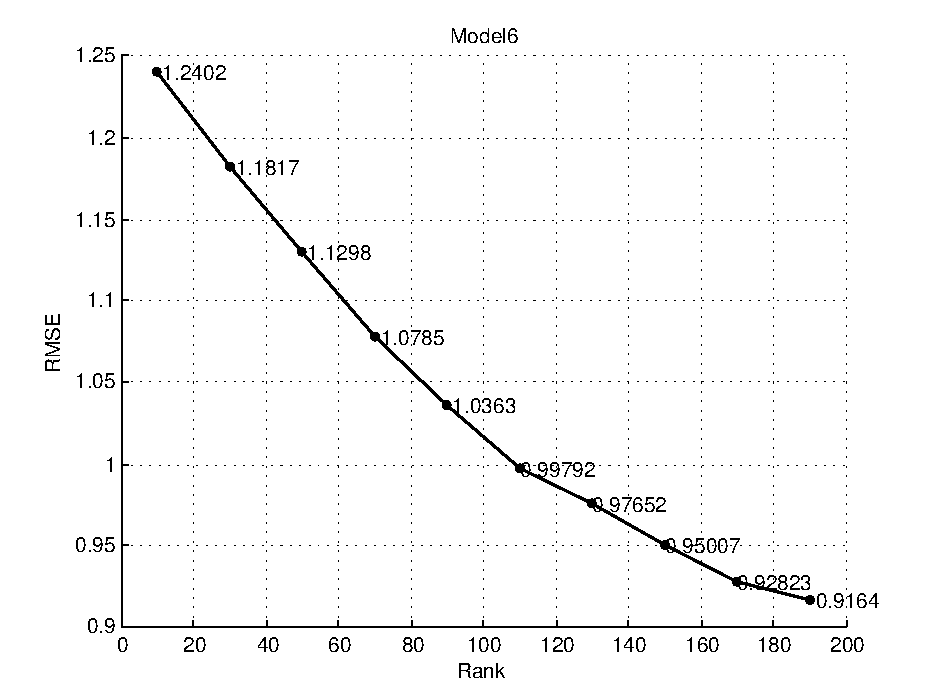
\includegraphics[width=0.45\textwidth]{./Results/plots/model6_1.pdf}
\label{fig:Model2}
}\\
\label{fig:RMSE SVD}
\caption{RMSE: ALS-I based models}
\end{figure}

\begin{figure}[h!]
\centering
\subfigure[RMSE for Model 7 for 30 iterations $N_f=200$]{
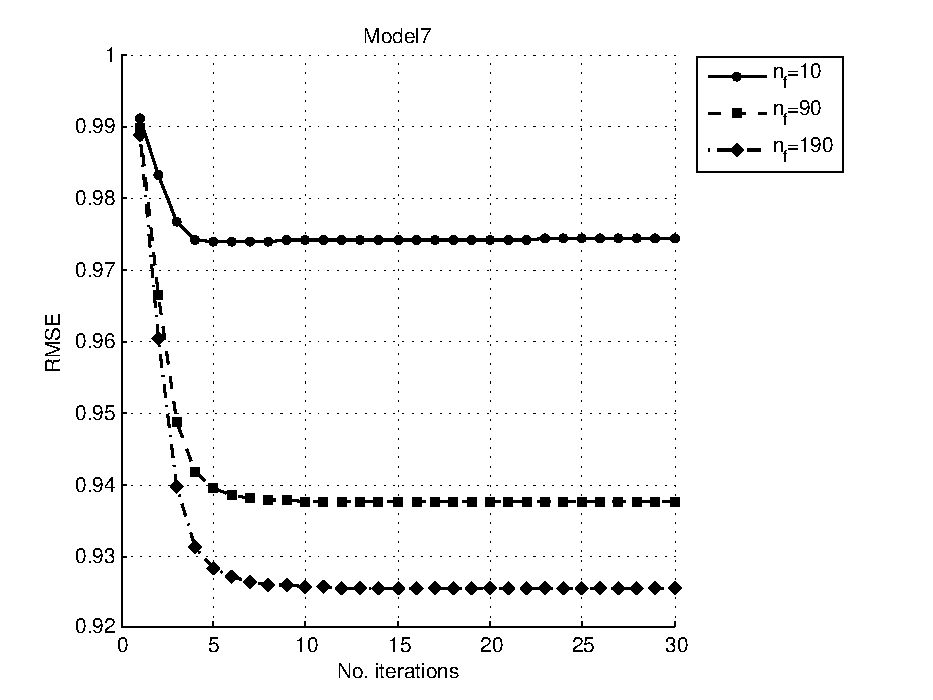
\includegraphics[width=0.45\textwidth]{./Results/plots/model7.pdf}
\label{fig:Model 1}
}
\subfigure[RMSE for Model 7 ]{
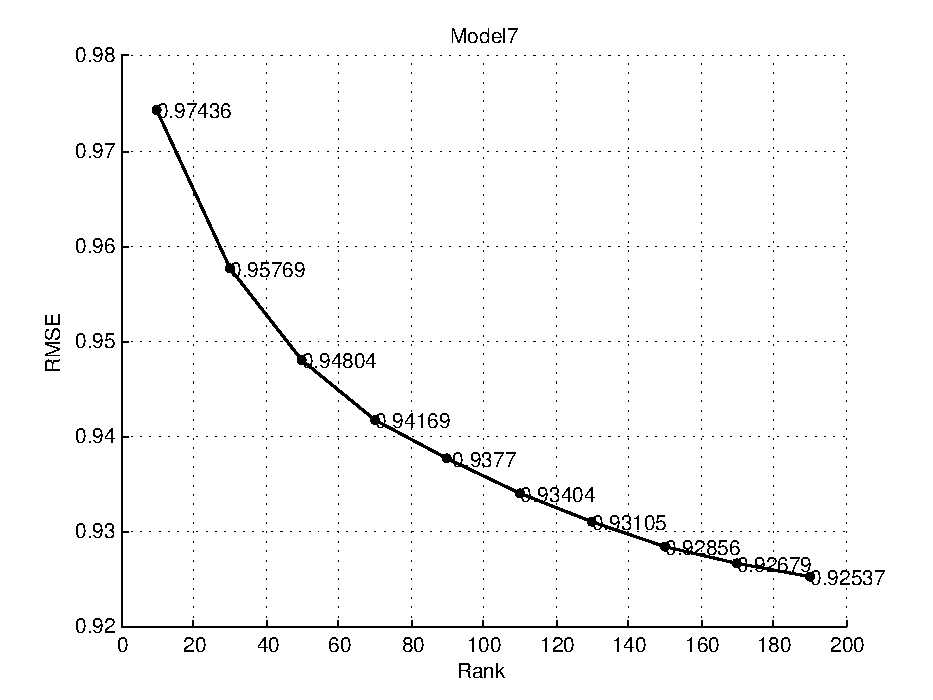
\includegraphics[width=0.45\textwidth]{./Results/plots/model7_1.pdf}
\label{fig:Model2}
}\\
\subfigure[RMSE for Model 8 for 30 iterations $N_f=200$]{
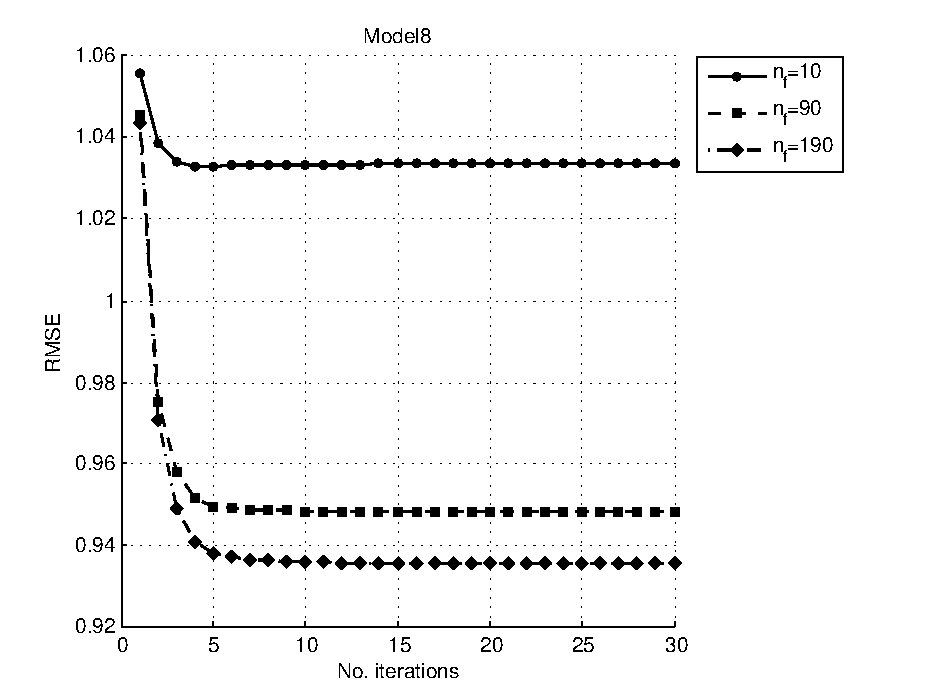
\includegraphics[width=0.45\textwidth]{./Results/plots/model8.pdf}
\label{fig:Model 1}
}
\subfigure[RMSE for Model 8 ]{
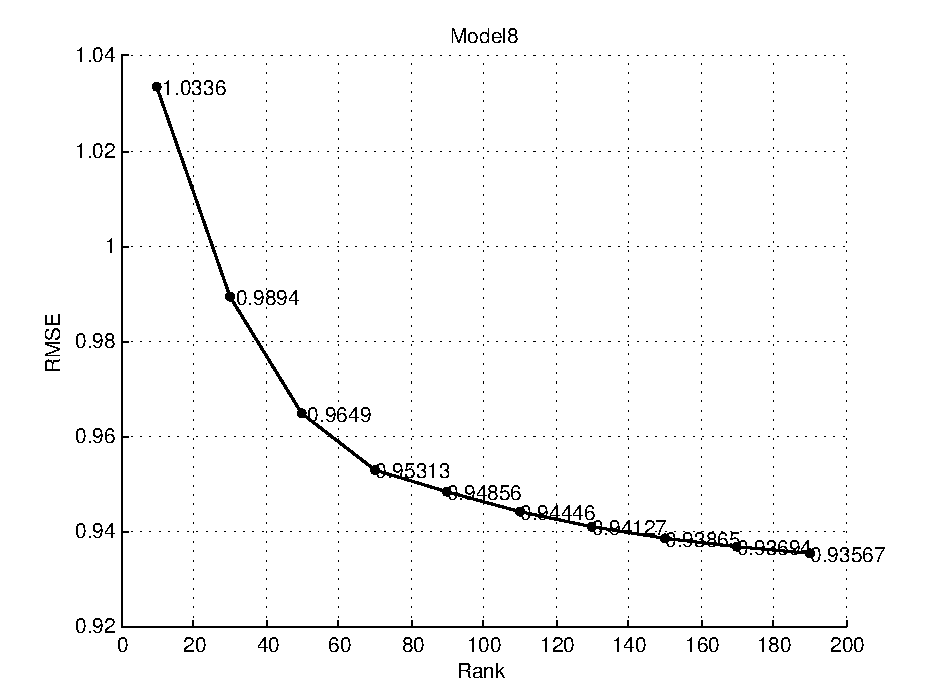
\includegraphics[width=0.45\textwidth]{./Results/plots/model8_1.pdf}
\label{fig:Model2}
}\\
\subfigure[RMSE for Model 9 for 30 iterations $N_f=200$]{
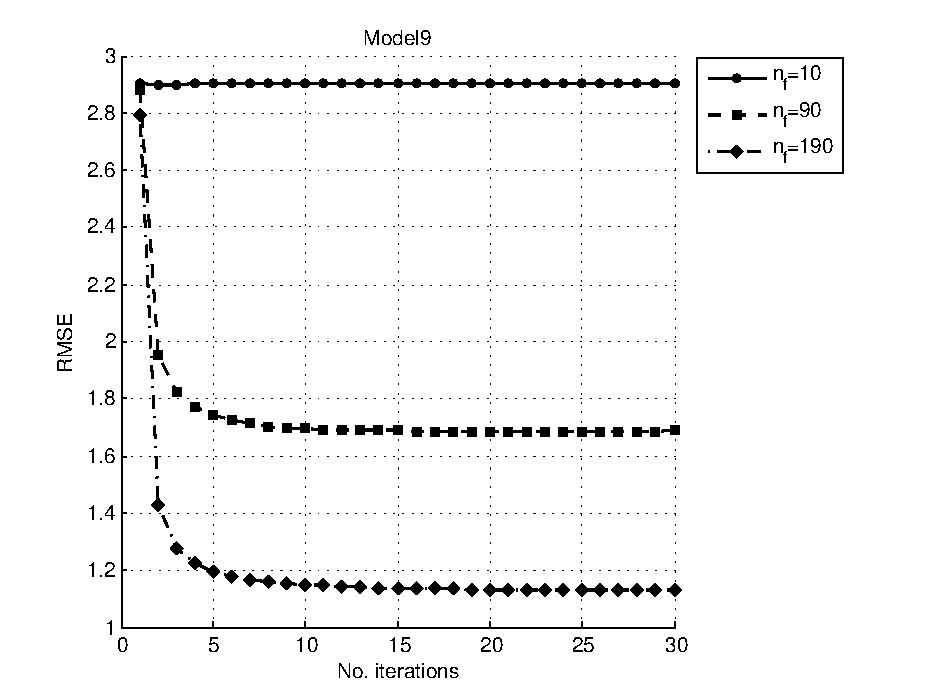
\includegraphics[width=0.45\textwidth]{./Results/plots/model9.pdf}
\label{fig:Model 1}
}
\subfigure[RMSE for Model 9 ]{
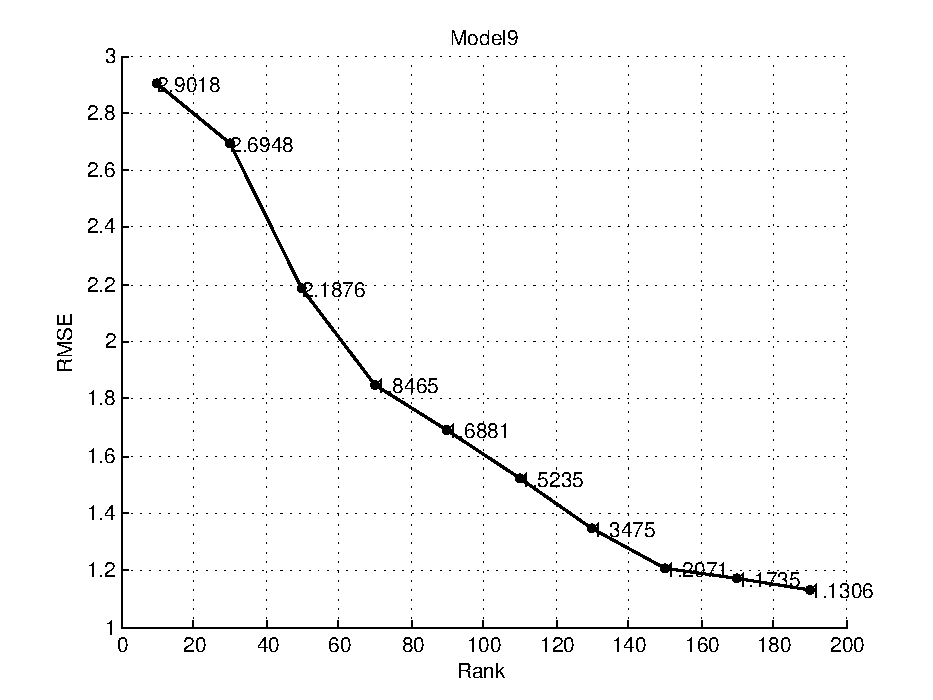
\includegraphics[width=0.45\textwidth]{./Results/plots/model9_1.pdf}
\label{fig:Model2}
}\\
\label{fig:RMSE SVD}
\caption{RMSE: ALS-II based models}
\end{figure}


\section{Future Work}
In this work we have only considered only movie related temporal effects. We
could for future work also include the more complex user realted temporal
effects. The user related temporal dynamics proves to be more comples and more
challenging to model. In a single household different people could be involved
in rating movies, and the mood and temperment of the user is susceptible to more
frequent changes. The user rates on forty different days on average. Apart from
the mood swings, the user could also alter the rating scale over time. We could
for further work consider the various user related effects and incude them into
the model in order to get more accurate predictions. 

Owing to the issue of unknown ratings being treated as zeros by the sparse SVD
of MATLAB, we have used an
alternative method. Instead it is possible to develop a factorization technique
based on SVD, but which is regularised. This approach was suggested initially by
Simon Funk \cite{Paterek_RegSVD}.

We could also aim to improve the prediction accuracy by considering inplicit
feedback. By doing so we can take advantage of additional information about user
preferences. In the current system, where we use only explicit ratings, where
there are users for whom we have very little information, implicit data could
prove to be useful \cite{citeulike:8923836}.









\bibliographystyle{plain}
\bibliography{bibl}

\backmatter
\appendix
\chapter{Sparse SVD Computation}
\label{app:SVDS}

\subsubsection{SVDS} 

This function in MATLAB computes the singular vectors and singular values of a given sparse matrix. \\


\subsubsection{Syntax} 

$[U,S,V]=svds(A,k),$ \\
where U is the \emph{right singular vectors} $m \times k$ matrix having orthnormal columns, \\
      V is the \emph{left singular vectors} $n \times k$ matrix having orthnormal columns, \\
      S is the $k \times k$ diagonal matrix, where the diagonal elements are the singular values. \\
      
\subsubsection{Description}
% \begin{left}
% \line(1,0){\textwidth}
% \end{left} \\
The MATLAB function svds uses Lanczos Tridiagonalization on the matrix,
\[
  B = \begin{pmatrix}
   0          &   A            \\
      A^T      & 0     \\

 \end{pmatrix}
\] \\


\begin{algorithm}
\caption{Lanczos tridiagonalization}
\begin{algorithmic}
Initialization: Starting vector $v_1$, such that $||v_1||_2=1$, $\beta_{0}=0$ and $v_0=0$.
 \For{$j=1,2,....$}
  \State$\alpha_{j}=v_j^{T}Av_j$.
  \State$v=Av_j-\alpha_jv_j-\beta_{j-1}v_{j-1}$
  \State$\beta_j=||v||_2$
  \State$v_{j+1}=(1/\beta_j)v$  
 \EndFor
\end{algorithmic}

\end{algorithm}





\end{document}
"
\end{codeexample}
\noindent where |main-figure0| is the picture we are currently externalizing and |main.tex| is the main document.

As soon as ``conversion mode'' has been detected, \pgfname\ changes the output routine. The complete file |main.tex| is processed as normal, but only the part of the desired picture will be written to the output file, in our case |main-figure0.pdf|. The rest of the document is silently thrown away. Of course, such a conversion process is quite expensive since we need to do it for every picture. Since everything except the current picture is thrown away, the library skips all other pictures. Furthermore, any |\includegraphics| commands which are outside of the converted \tikzname-picture will be skipped as well. Thus, the conversion process should be much faster than typesetting the complete document, but it still requires its time.
Eventually, the call |\documentclass[mai, 10pt, english, crop, info, print]{liuthesis}

% Pasted from Niklas main.tex
      \usepackage{amsmath,amssymb}
      \usepackage[table]{xcolor}
      %\usepackage{makeidx}
      \usepackage{savesym}
      \savesymbol{AND}
      %\usepackage{algorithmic}
      \usepackage{algorithm}
      %\usepackage{tikz}
      \usepackage{pdfpages}
      \usepackage{subfigure}
      \usepackage{graphicx}
      \usepackage{algpseudocode}
      \usepackage{algorithmicx}
      %\usepackage{hyperref}
      
      %\usetikzlibrary{positioning,chains,fit,shapes,calc}


      \DeclareMathOperator{\diag}{diag}
      \DeclareMathOperator{\rank}{rank}
      \newcommand{\x}{\times}
      \newtheorem{proposition}[theorem]{Proposition}
%

\author{Abhijith Chandraprabhu}
\title{Collaborative Filtering using Temporal Analysis}{Svenk Titel}

\thesisDate{9}{19}{YYYY}
\thesisNo{LiTH-MAT-EX{-}{-}YY/XXXX{-}{-}SE}

\thesisDivision{Division of Applied Mathematics}
\URL[http://math.liu.se]{http://www.ep.liu.se}

\subject{Department of Mathematics}
\keywords{Netflix, Recommender Systems, RMSE, Matrix factorization, Sparse SVD,
ALS-WR, Low-Rank Approximation,}

\examiner{
  Lars Eld�n \AT \textsc{mai}, Link�pings universitet}

\supervisor{
  Berkant Savas \AT \textsc{mai}, Link�pings universitet}

\abstract{In todays digital world Information in the form of large scale data
has become a very important source of knowledge, this is largely owed to the
advances in Data Sciences. One of the recent applications of data mining is to
find meaningful and useful relationship between groups of entities, for
example between users and movies as in the case of NETFLIX. With the NETLIX
competition, the field of Recommender Systems which helps in presenting users
with relevant items based on the history rather than an explicit search query,
has generated great interest from researchers and this work is one such attempt.
When we talk about users' preferences it is natural that it evolves, hence in
this work we have tried to account for a new dimension, i.e time, while building
the model. On the lines on the NETFLIX competition, the task of predicting
preferences involves the ratings of the movies given by users and it is the
value of this rating which we try to predict. On the lines on the NETFLIX
competition, the task of predicting preferences involves the ratings of the
movies by users and it the value of this rating which we try to predict. The
data upon which the algorithm is built consists of around 1 million ratings
given by around half a million users to around 18k movies. Collaborative
Filtering techniques have been employed, where based upon a model which has
information of users and movies we try to fetch prediction of new ratings by
factoring the user space and movie space and finding a relationship between the
required pair. Matrix factorization is done based on Singular Value
Decomposition, and owing to the inherent nature of SVD to handle
sparse data inefficiently an alternate method based on Alternate Least Squares
was used.}

\acknowledgements{ Parents, Berkant Savas, Lars Elden, Niklas Ekvall, Opposition person.}
%\useHyperRef

\begin{document}

\makeFrontMatter

\chapter{Introduction\index{Introduction}}


\textsf{%
In this chapter we introduce the field of Datamining and its relevance. We
also introduce the area of research in which this thesis work is done.}

\section{Introduction\index{Introduction}}
The field of Data Mining aka Knowledge Discovery in Data, or KDD saw its first
light during the 1990s, and has evolved along with the processing power and
storage capacities of modern computer systems. The amount of data only from the
web is in the order of exabytes and continues to increase, this along with other
sources of data resulting from reserach and experimentation proves to be one the
most important sources of knowledge. The data mining techniques are applied
to wide variety of applications like in business, to improve customer
relationhip management, or to do market analysis with respect to a particular
product. The medical fraternity use them to do temporal analysis of patterns
concerning drug presciptions to diagnoses. With respect to science and
engineering, DNA sequence mining proves very crucial in understanding the
variations in human DNA. Data mining actually can be seen as one step towards
discovering knowledge from raw source, initially there are many more processes
like understanding of the application domain and collecting the data, then there
is data transformation and only then is the actual data mining techniques
applied. Even after the data is mined and clusters or patterns are obtained,
interpretation of these patterns and taking required actions forms the last
stage. There are six main tasks within the gamut of data mining, enlisted
below, \cite{Fayyad96fromdata}
\begin{description}
  \item[Classification] is learning a function that maps a data item into one of
several predefined classes.
  \item[Regression] is learning a function that maps a data item to a
real-valued prediction variable.
  \item[Clustering] is a common descriptive task where one seeks to identify a
finite set of categories or clusters to describe the data.
  \item[Summarization] involves methods for finding a compact description for a
subset of data.
  \item[Dependency Modeling] consists of finding a model that describes
significant dependencies between variables.
\item[Change and deviation detection] focuses on discovering the most
significant changes in
the data from previously measured or normative values.
\end{description}

  The kind of prediction we are dealing with is ratings prediction, which gives
an indication of user's preference to items. Depending on the predicted rating
recommendations are made, this involves different tasks the most significant of
them being matrix factorization and rank reduction. It is very common while
dealing with preferences that they tend to change with time, the work by
\cite{Koren:2010:CFT:1721654.1721677} models the data drifting with time. It is
important to note that while modeling temporal effects we should take into
account there are transient signals analogous to users and a more long term
patterns characterized by movies.



\chapter{Collaborative Filtering\index{Collaborative Filtering}}


\textsf{ In this chapter we explain Collaborative Filtering in more detail,
along with giving details of the NETFLIX prize and the lead up to present work.
We explain about the data and the approach to the solution of the problem.}


\section{Recommender Systems\index{Recommender Systems}}
Internet technologies have greatly become a part of our lives, there are many
occasions when we need help in taking certain decisions. Recommendations in
general is ubiquitous when there is a need to make choices without sufficient
personal experience, we rely on feedback from users on certain products, we make
use of recommendation letters for jobs, reviews of movies and books
\cite{Resnick:1997:RS:245108.245121}. Consider for a movie streaming company
like NETFLIX, where people can watch movies from a huge collection, have been
collecting the ratings of the movies from the users. This data can be considered
as our \emph{training data}, it is explicitly obtained from the users. Using
this training data the company makes predicitions of movies the users are likely
to prefer watching more than others. This is only one of the different types of
recommender systems. 
\subsection{Recommender System Strategies}
The strategies for building recommender systems are based on the type of data
available and how the data is used. On a broad sense the two main approaches are
\emph{content-based filtering}, in which the items are characterized based on 
certain attributes, and recommendation are made based on filtering similar
items. In the second approach, \emph{collaborative filtering}, the ratings
previously given by users is used to build a model, which is then used to make
predictions. The term Collaborative Filtering was first termed by Tapestry
\cite{Goldberg:1992:UCF:138859.138867}, which was one of the first recommender
systems. Recommender
Systems produce possibly accurate prediction of relationship between elements of
different classes based on previous knowledge or the \emph{training data}. This
training data could be explicitly obtained in the form of ratings given by
users or it could be implicit knowledge(purchase
history, browsing history, search patterns,mouse movements etc), which can be
used when explicit knowledge is insufficient \cite{Hu:2008:CFI:1510528.1511352}.
But however in this thesis work we model our system based on explicit
knowledge. 

Modern recommender systems are based on the collaborative filtering, which again
is of two types, the \emph{nearest neighbor approach} and the \emph{latent
factor approach}. In the nearest neighbor methods, items or users are given
certain attributes which decides the proximity between them. Further this sense
of proximity is used predict an item for an user. The second approach is
the latent factor approach, which characterizes the users and the items together
in building the model. Matrix factorization is used to build these models, likes
of SVD is very useful. \emph{Rating matrix} proves to be important, as it
charectarizes both items and users as its vectors. 

\subsection{The Problem Formulation}
Our problem could be defined as a matrix completion problem, where the matrix is
formed by placing the users $u$ along the rows and the movies $m$ along the
rows. The entries in this matrix are filled through the \emph{training data},
which is collection of $n$ \emph{quadruples}, with the format
(\emph{user(k)},\emph{movie(k)},\emph{rating(k)},\emph{timestamp(k)}), where
$k=1,2...,n$. The $1 \leq user \leq u$ and $1 \leq movie \leq m$ are the
range of the users and the movies, where as the ratings, $1<rating<5$. The
\emph{Rating
matrix} is defined as $R\in\mathbb{R}^{u,m}$, \\
\begin{equation}
  R[i,j]=\begin{cases}
    rating(k), & \text{$i=user(k), j=movie(k)$}.\\
    ?, & \text{otherwise}.
  \end{cases}
\end{equation}

where \emph{'?'} are the cases where the \emph{user-movie} relation is unknown.
These are the values which needs to be predicted. Once the \emph{'?'} values are
computed, recommendations could be made depending on the required tolerance
level, \emph{user-movie} pairs with predicted ratings higer than the tolerant
value(threshold) can be selected for making recommendations. Hence this problem
can be viewed as a \emph{matrix completion} problem. In this thesis work, we
will compute the unknowns for a certain subset called the \emph{test set}. \\

Let us denote the completed matrix, or rather the reconstructed matrix	 by
\emph{$\hat_{R}$}. We intend to obtain the
\emph{$\hat_{R}$}, by reproducing it through a simple product of two matrices
with reduced \emph{inner dimension}. Let $P\in\mathbb{R}^{u,f}$ and
$Q\in\mathbb{R}^{f,m}$ are the two matrices with reduced inner dimension
\emph{f}. 


Let us through a very simple example see the principle behind collaborative
filtering.

 \begin{example}
   We show 4 users who have rated 4 movies, we tabulate the preferences, in the
form of ratings on the scale of 1 to 5,  as shown below. The users are along the
rows and items along the columns, rating  given by \textit{user i} to
\textit{item j} is the real valued entry (i,j) in  the rating matrix.  \\

\begin{tabular}{c|cccc}
       & Titanic & Braveheart & The Lion King & Dreamcatcher  \\
\hline
John   & 5 & 5 & 2 & -   \\
Dave   & 2 & - & 3 & -   \\
Alice  & - & 5 & - & 3   \\
Bob    & 3 & - & - & 5   \\
\end{tabular}

From the above, we can consider the rating matrix to be \\

$R_{i,j}$ =
$ \begin{pmatrix}
  5 & 5 & 2 & ? \\
  2 & ? & 3 & 5 \\
  ? & 5 & ? & 3  \\
  3 & ? & ? & 5
 \end{pmatrix} $\\
 
 Using matrix factorization, we simply do a SVD on $R$ to get, $U$ and $V$,
which denote the user space and the movie space. \\
 
 $U$ =
 $\begin{pmatrix}
  1.12 & 1.49 & 0.48  \\
  1.31 & -0.52 & 0.59  \\
  1.13 & 0.67 & -0.52  \\
  1.39 & 0.05 & 0.45 
 \end{pmatrix} $
 \hspace*{10mm}
 $V$ =
 $\begin{pmatrix}
  1.12 & 1.49 & 0.48  \\
  1.31 & -0.52 & 0.59  \\
  1.13 & 0.67 & -0.52  \\
  1.39 & 0.05 & 0.45 
 \end{pmatrix} $\\

 Once we have factored the rating matrix $R$, we can get the missing values by
approximating the sparse rating matrix into a full one,  $\hat{R}=U*V'$ \\

$\hat{R}_{i,j}$ =
 $\begin{pmatrix}
  4.78 & 4.98 & 1.97 & 3.61 \\
  1.98 & 1.97 & 2.85 & 4.81 \\
  2.75 & 4.71 & 1.40 & 2.94  \\
  2.94 & 3.32 & 2.75 & 4.79
 \end{pmatrix} $\\
 
 With this approximation, we can make predictions of ratings of movies which the
users have not seen. 
 
\end{example}

\section{NETFLIX}
Entertainment has been one of the most significant integral part of human
society and has evloved along with modern technologies. In todays internet
driven society, IPTV(Internet Protocol Television) is gaining popularity in
delivering television and cinema content to viewers. IPTV mainly consists of
three groups, \\
\begin{enumerate}%for small alpha-characters within brackets.
\item Live Television - Live telecast or transmission to the viewers with only
the transmission delay, example live news show.
\item Time-shifted Television which is also called as catch-up TV, in which the
viewers can watch the content which is stored and available at any point of
time. 
\item Video on Demand - here the viewers are given a wide range of TV shows and
movies to choose. They can watch anything they wish, the content is streamed to
the viewers computer which the user can pause and watch later. NETFLIX provides
its content throught this method. \\
This owes to a great extent to the success of NETFLIX, since through on Demand
system NETFLIX is able to cater to individual tastes of users. NETFLIX can
collect statistics pertaining to individual users' choices and the most
important metric is the \emph{ratings}. NETFLIX aims to greatly improve the
customer satisfaction and retention by providing a greatly personalised
experience to the users. The importance of personalization is such, that NETFLIX
ignited the research attempts in the Mathematical and Computer Science soceity
to develop methods which could do predictions for movie likeability quotient.
Such attempts have certainly been fruitful to NETFLIX as is evident from the
fact that as of today 33 million members view over 1 billion hours of TV shows
and movies through NETFLIX per month.
\end{enumerate}

\subsection{NETFLIX Prize}
During October 2006, NETFLIX challenged the research community to beat the
performance in terms of accuracy of their own recommendation system
\emph{Cinematch} by 10\%. The NETFLIX prize challenge was provided with over 100
million ratings from around half a million users and 18 thousand movies. This
data was collected during the period october 1998 and December 2005. The
challenge would take place over a period of three years, and a progress prize of
50 thousand USD would be awarded each year to the team which would produce the
best improvements. Finally at the end of three years a Grand Prize of 1 Million
USD would be given to the team with the best results in terms of RMSE. Their
benchmark system \emph{Cinematch}, based on \emph{Pearson correlation} which is
straightforward statistical linear model produces an RMSE of 0.9525 on test
data. Hence to qualify to win the Grand Prize which accounts for 10\%
improvement over \emph{Cinematch}, which corresponds to RMSE of 0.8563 on
\emph{quiz set}. On an event of a tie the time of entry would be taken into
account, and this is exactly what happened on 26 July 2009, team BellKor's
Pragmatic Chaos won the challenge by margin of 20 minutes. Table 2.1 shows the
performance of top 12 teams, \cite{NETFLIX_Prize:Online}
\begin{table}
\centering 
\begin{tabular}{|c|c|c|c|} \hline %\hline
%-------------------------------------------------------------------
$Rank$ & $Team$ & 
$RMSE$ &  $Percent Improvement$  \\ 
\hline
%-------------------------------------------------------------------
$ 1$
& $BellKor's Pragmatic Chaos$
& $0.8567$
& $10.06$ \\ %\hline
%-------------------------------------------------------------------
$ 2$
& $The Ensemble$
& $0.8567$
& $10.06$ \\ %\hline
%-------------------------------------------------------------------
$ 3$
& $Grand Prize Team$
& $0.8582$
& $9.90$\\  %\hline
%-------------------------------------------------------------------
$ 4$
& $Opera Solutions and Vandelay United$
& $0.8588$
& $9.84$\\  %\hline
%-------------------------------------------------------------------
$ 5$
& $Vandelay Industries !$
& $0.8591$
& $9.81$ \\%\hline
%-------------------------------------------------------------------
$ 6$
& $PragmaticTheory$
& $0.8594$
& $9.77$ \\ %\hline
%-------------------------------------------------------------------
$ 7$
& $BellKor in BigChaos$
& $0.8601$
& $9.70$ \\ %\hline
%-------------------------------------------------------------------
$ 8$
& $Dace$
& $0.8612$
& $9.59$ \\ %\hline
%-------------------------------------------------------------------
$ 9$
& $Feeds2$
& $0.8622$
& $9.48$  \\%\hline
%-------------------------------------------------------------------
$ 10$
& $BigChaos$
& $0.8623$
& $9.47$ \\ %\hline
%-------------------------------------------------------------------
$ 11$
& $Opera Solutions$
& $0.8623$
& $9.47$ \\ %\hline
%-------------------------------------------------------------------
$ 12$ 
& $BellKor$        
& $0.8624$ 
& $9.46$  \\ \hline 
\end{tabular}
\caption{RMSE of Top 12 Teams}
\label{tab:TopTeams}
\end{table}
-
\subsection{The NETFLIX dataset}
NETFLIX had been collecting data since October 1998,
as of June 2007 the company had collected over 1.9 billion ratings from more
than 11.7 million subscribers over 85 thousand titles \refname{The NETFLIX
Prize}. The company then recieved over 2 million ratings per day. To provide
data for the competition the company did two seperate random sampling processes,
the first one to obtain th eentire Prize dataset and second for the qualifying
and probe set. The condition for selecting the users was that they should have
given minimum of 20 ratings. \\

 Basically the company has seggregated the data based on time, the latest data
form the Test Data and the initial data form the training data. The
\emph{Training data} includes the \emph{Probe set} which is meant for fine
tuning before submissions. The training data is basically a text file consisting
of triplets entries like, (UserID, MovieID, Rating). There are 100 million such
entries which form the training set. The training set also included the probe
set consisting of 1,408,395 triplets, this could be used by the competitors to
fine tune their algorithms before submission. NETFLIX also collected the latest
ratings of all the users in the training set to form the \emph{Qualifying set}.
This set was in the form (UserID,MovieID,DatrofRating), where the ratings were
known only to the judjes. The qualifying set was again divided into 2 groups,
the \emph{Quiz set} and \emph{Test set}. The quiz set having 1,408,342 ratings
was used to update the Leaderboard, the RMSE on this quiz set was released to
the competitors. The test set having 1,408,789 ratings was only used by the jury
to adjudge the winner. \cite{Bennett07thenetflix}\\



 
\begin{table}
\begin{center}
    \begin{tabular}{|ccc|}
        \hline
         TRAINING SET  & ~ &  Probe set  \\ 
         100480507 & ~ & 1408395   \\ \hline       
    \end{tabular} \\
    \caption[]{Training Data}
     \begin{tabular}{|c|c|}
       \hline
       Test Set  & Quiz Set  \\ 
       1408789 & 1408342 \\ \hline       
    \end{tabular}
    \caption{Qualifying Data}     
\end{center}
\end{table}


\section{Matrix Factorization for Collaborative Filtering}
With Collaborative Filtering it involves filtering for information through
collaboration among interacting groups, for example users and movies. Matrix
factorization happens to be the first choice for collaborative filtering, as
matrices can hold high dimensional information in tabular form, and can be
factored into products of smaller matrices. \emph{In matrix factorization the
users and items are mapped onto a joint latent factor space of reduced dimension
$f$, and the inner product of the user vector with item vector gives the
corresponding interaction.} \cite{Koren:2009:MFT:1608565.1608614}
\subsection{Basic Matrix Factorization}
Matrix factorization is mainly about a more compact representation of the large
training data which is obtained by dimensionality reduction.
\cite{Liu:2010:GLA:1821715.1821722}. 
\emph{We want to quantify the nature or the characteristics of the movies
defined by a certain number of aspects (factors), i.e we are trying to
generalize the information (independent and unrelated ratings matrix) in a
concise and descriptive way.} \cite{citeulike:4563139} All the movies can be
described by certain features like overall rating, cast, wether its an action
flick or romantic drama, how did it fare during the first week of it release
etc. Similarly a user can also be described based on the same factors, wether
the user is liberal in rating or very critical, does the user have certain
favourite cast, if the user prefers action over romance, does the user watch and
rate movies on the first week of its release etc. What we have here is a common
factor space in which we tend to generalize the relationships between the users
and movies, based on these factors. Hence the 8.5 billion ratings can be
explained in lot fewer factors. We are generalizing the independent individual
unrelated ratings to a more concise and descriptive form. Here what we have done
is through meaningful generalities, concised the data, the reverse also holds
good, i.e by concising the data or in other words by reducing the dimension, we
can generalize the description of the large data. The Singular Value
Decomposition exactly helps in achieving this. This is explained crudely with an
example,\\

\begin{example}
Let us say we have around ten aspects which are used to describe movies and
users. Each movie has ten numerical values, which exemplifies the ten aspects.
Similarly the users also have ten such values. We can combine these values to
obtaing a single rating value for each user-movie pair, bu multiplying the
corresponding terms and summing them up. Let us consider a movie Die Hard whose
aspects might be something like, action=1.2, chickflick=-1, and so on. Let us
consider a user Joe whose aspects are, action=3, and chickflick=-1. So the
overall rating for the movie Die Hard given by Joe is, $3*1.2+-1*-1+..$ =
$(3.6+1+..)$. It clearly shows that Joe would evetually like the movie Die
Hard, which is evident from the high rating value obtained.   
\end{example}\\

 The model in its most basic form is built around the following \\
 $R=P*Q'$
 where $P\in\mathbb{R}^{u,f}$ and $Q\in\mathbb{R}^{i,f}$. The number $f$ is
decided by trial and error, higher the value better the predictions, however
beyond certain value it will not contribute to the accuracy significantly. This
value decides the number of \emph{factors} which will be used to characterize
users and movies. This is analogous to dimension reduction. \\
The individual vector in $P$, $p_{u}\in\mathbb{R}^f$ represents an user, it
gives a measure of the qualities represented by the $f$ factors. Similarly,
every item is represented by a $q_{i}\in\mathbb{R}^f$ which says about the $f$
qualities pertaining to the items, i.e movies. We cannot for sure say what are
the qualities which these factors represent. The task of predicting a rating
for a user $u$ gives for a movie $i$, can be computed as an inner product, \\

$\hat{r}_{ui}=q_{i}^Tp_{u}.$ \\

This dot product gives the iteraction between the item $i$ and the user $u$. The
challenge is in the mapping of all the users and items to a joint latent factor
space of dimensionality $f$ \cite{Koren:2009:MFT:1608565.1608614}.\\
Singular Value Decomposition (SVD), would be first choice for such a
factorization, as it helps a great deal in identifying the the best top-most
factors, i.e by selecting the left and right singular vectors corresponding to
top $n$ singular values. \\

\subsection{Dimension Reduction}
Matrix factorization and dimension-reduction go hand-in-hand, the dimension of
our rating matrix is very high and along with factorizing the matrix it is
important to reduce the dimensions of the factored matrices. It is the inherent
property of SVD that we can decide the rank or the number of \emph{factors} we
need in order to get the best approximation of our User-Movie rating model. By
dimension reduction we get to express the information which was initially
presented
in a matrix of dimension 480189x17770 having around 85 billion ratings in much
smaller space with only \emph{k} factors, where \emph{k} is the reduced
dimension.
While a reduction in dimension, also aids in removal of noise, however too low
dimension
can result in removal of useful information as well. Hence it is important to
decide on an optimal dimension. Through an example below we can further justify
the
need for dimension reduction,
\begin{example}
 Consider movies like "Harry Potter", "Chronicles of Narnia", "Lord of the
Rings" etc, there are very large number of movies similar to this. By saying
similar what we mean is that these movies all have certain common factors, like
they all are fantasy movies, they all are novel based movies. Hence instead of
retaining all these movies, we can replace them with certain latent factors,
which are much fewer than the number of items or movies, and hence the dimension
is reduced.
\end{example}


\subsection{Different Models}
Collaborative Filtering based Recommender Systems are built using either
Neighbourhood-methods or model-based methods
\cite{Koren:2008:FMN:1401890.1401944}. Our approach involves the
model-based method, which has proved to be one of the most effective approach as
is evident from the NETFLIX Challenge and large number of research articles on
the same topic. To have a good Recommender System, it is important to achieve
good accuracy and also to keep the model simple. Keeping this in mind, we try to
build a model which accounts for significant predictor variables, like the
temporal dynamics, user-bias, movie-bias etc. However we initially analyze these
individual predictors and after careful analyses, we blend them together in the
final model to achieve the best RMSE. The main principle behind our model of
laten factor modelling, supplemented with the removal of biases pertaining to
users, movies and temporal variations. Below table shows the various models we
use, 

\begin{table}
\centering 
\begin{tabular}{|c|c|} \hline %\hline
%-------------------------------------------------------------------
$Model No.$ & $Model$   \\ 
\hline
%-------------------------------------------------------------------
$ 1$
& Naive Models based on user/movie means  \\ %\hline
%-------------------------------------------------------------------
$ 2$
& Bias-Model\\ %\hline
%-------------------------------------------------------------------
$ 3$
& Temporal model - SVD  \\ %\hline
%-------------------------------------------------------------------
$ 4$
& Temporal model - ALS  \\ \hline
%------------------------------------------------------------------- 
\end{tabular}
\caption{Different models}
\label{tab:Models}
\end{table}


\subsubsection{Data Representation}
Before beginning discussion on the models, we show a detailed representation of
the training and the test data which are used in this work, which are in the
form of matrices, i.e, the rating matrix $R$, the date matrix $D$,
these comprise the training data. The test data is in the form of three
matrices, probe set $P_{probe}$, test set $Q_{test}$, quiz set
$Q_{quiz}$ and finally $Q_{all}$ which consists of the entire test
data. Each of the above matrices except $D$ are in the form,  \\
$\mathcal{R} = \{r_{ij} \exists \mbox{ in } R \mid \mbox{user } i \in
\mathcal{U} \mbox{ have rated movie } j \in \mathcal{M} \}$, \\
where $r_{ij}$ is the rating for the corresponding user-movie pair and is also
the $(i,j)^{th}$ entry in their respective matrices. The matrix $D$ however
has the same structure of $R$, but with the date of rating instead of the
rating itself.

\subsubsection{Basic Naive model} We start by doing some rating predictions
based on the average of all the ratings in the $R$ matrix, which is 3.5769. We
simply use this value for any unknown user-movie combination. Moving ahead we
could use the \emph{user-mean}, to calculate the unknown rating, for example if
we need a prediction for user $u$, for any of the movies we simply use the
average of all the ratings given by user $u$. Similarly to predict the unknown
rating for some movie $i$, we could simply use the average rating of that movie
over all the known ratings given to that movie in the matrix $R$.  
\subsubsection{Bias model} Moving ahead we try out new models which takes care
of the inherent biases of various kinds in the data. Bias model removes the
anomalies, if any in the data. Biases in this cintext can be considered to be
variations in the ratings which are caused by certain effects associated with
the users or movies, independetly of the interaction between the two groups.
The interaction is captured in the factorization part and the inner products of
the interacting vectors. The main purpose of doing this is, by separating the
interaction and the biases will help us in subjecting only the interaction
portion of the data which is more critical
\cite{Koren:2010:CFT:1721654.1721677}.
The $Baseline predictors$ capture these biases which do not involve user-movie
interaction. While factorization these biases are removed only to be added after
factorization, i.e, post-processing. 
\subsubsection{Temporal Bias + SVD model} The main objective in this thesis is
to capture the temporal dynamics within the data and include them into the
$baseline predictors$ through two major temporal effects, each involving users
and movies. However in this thesis the temporal effects related only to movies
is considered. We have considered the movie-bias to be a function of time, which
can capture the changes in popularity of movies in course of time, owing to
number of external triggering factors like the actor in the movie winning a
major award. Also the users tend to drift with their rating styles with time,
for example a liberal user might for some reason become a more critical in
rating movies. \\
 This model uses the good old Singular Value Decomposition for the factorizing
the rating matrix. But however it is evident that owing to the sparsity in the
data SVD proves to be not very effective. To avoid this imputation can be
employed but this can be very expensive in terms of memory. 
\subsubsection{Temporal Bias + ALS model} Owing to the disadvantage of the SVD
as will be explained in future chapters, we employ an alternative method in
Alternating Least Squares. It is an iterative method with initial guessed
values for $M$ and alternatively solving for $U$ and $M$ until convergence. This
method is computationally demanding but can be parallelized easily. If $R$ is
the rating matrix, we formulate a low-rank matrix approximation problem as shown
below,
\begin{equation}
 (U,M)=arg \min_{U,M} \mathcal{L}^{\emph{emp}}(R,U,M)
\end{equation}
where $U$ and $M$ $\in \mathbb{R}$ and have $n_f$ columns. The symbolic
representation of the problem is shown below,


The $x^s$ denote the known ratings in the matrix $R$ and $\in \emph{I}$, where
\emph{I} is the known ratings set and $n$ is the number of known ratings in
total. In general the problem is of the type, 
\begin{equation}
 \|{Ax-b}\|
 \label{eq:OLS}
\end{equation}
\begin{equation}
 \|{R-UM^T}\|
 \label{eq:ALS}
\end{equation}
where we are trying to minimize the above in Frobenius norm, which is matrix
equivalent of 2-norm. We wish to solve the above problem in a least squares
sense, but since it is not in the form of ordinary least squares(OLS). We try to
convert the type shown in Equation ~\ref{eq:ALS} to the type shown in Equation
~\ref{eq:OLS}.
\begin{figure}[h!]
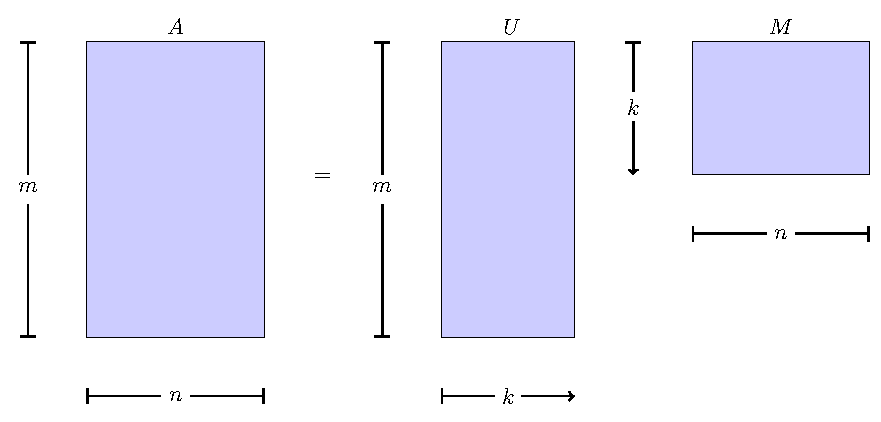
\includegraphics[width=1\textwidth]{ALS_FIG.pdf}

\caption{ALS Decomposition}
\label{fig:ALS Decomposition}
\end{figure}


Let us consider the first row of $R$, which will have all the ratings
given by the fist user. Let us assume the user has seen movies 1, 213, 315,
1744, 2133, 7044, 9012, 12344 and 16890  so in a total of 9 movies. Forming a
vector of the known ratings for the first user we have $\begin{bmatrix}
                                          1 & 213 & 315 & 1744 & 2133 & 7044 &
9012 & 12344 & 16890                                    
                                          \end{bmatrix}
$, let
this be denoted by $b$. We initialize the $M$ matrix in a particular way, and as
shown in the Figure 2.1 it has $n_m$ rows and $n_f$ columns. The matrix $U$ has
$n_u$ rows and $n_f$ columns. For the case of the first user we can form a
sub-matrix of $M$, denote this by $M_u$. This matrix $M_u$ will have all the
rows from $M$ corresponding to the movies seen by the user $u$, the first user
in this case. Let $\boldmath{u}$ be the row vector from $U$ corresponding to the
considered user, .i.e, first user. Now we have three components $R(1,:)$, the
row vector having the nine ratings of the nine movies seen by user 1, $u_1$ the
unknown first row of $U$ matrix, $M_u$, a submatrix of $M$ consisting of the
rows corresponding to the movies rated by the user 1. Figure 2.2 shows the
symbolic representation of this single ordinary least squares problem
formulation, $ \|{M_uu-R(1,:)}\|$. This is done for all the users to obtain the
$U$ matrix. Next this $U$ matrix is used to estimate the new $M$ matrix. The $U$
and $M$ are estimated alternatively until some convergence criteria is
satisfied. 


\begin{figure}[h!]

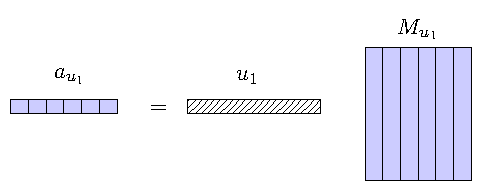
\includegraphics[width=0.6\textwidth]{ALS_FIG2.pdf}
\caption{OLS }
\label{fig:OLS Decomposition}
\end{figure}










\chapter{Temporal Dynamics\index{Temporal Dynamics}}



\textsf{ In this chapter we explain all the aspects related to Temporal Dynamics
in the NETFLIX data. We also show how to build temporal bias based model.}

\section{Temporal Dynamics in NETFLIX data}
The main goal in this work is to integrate temporal information into the
Recommender System model we are building based on collaborative filtering. It is
very important to consider temporal dynamics since the vast amounts of data we
are flooded with is dynamic in nature, and most of the information retrieval
tools today consider only the snapshot of this data, thereby loosing one very
potential dimension. In this chapter we present in detail the significance of
temporal dynamics in general and with respect to NETFLIX and also how to include
temporal dynamics into the model. \\


Since we are trying to improve the prediction rate by including temporal
effects, it is very critical to identify and uncover all possible temporal
effects within the NETFLIX data. This section summarizes and reports the
temporal analysis of the NETFLIX data.

\section{Tracking Drifting Customer Preferences}
The phenomena of $Concept drift$ is evident in the case of NETFLIX system, as we
can see that the user preferences of movies keep changing over time due to
various reasons. Concept drift means when the statistical properties of the
target variables change with time, like how user preferences change with new
release of new movies. In our case where we are trying to collaborate using
interconnected preferences among users, it is a challenge since each of the
interacting users could be drifting in different ways and also they are in
different time instances. There are mainly three kinds of approaches to include
time apect, \emph{instance selection}, in which only the recent instances are
considered, discarding off other instances. All instances within a specific time
period is given equal opportunities discarding instances ouside this period.
This obviously leads to lose of information.  In 2005, a time-weighted CF method
was proposed by Ding and Li in \cite{Ding:2005:TWC:1099554.1099689}, in
which depending on how recent the ratings are they are weighted accordingly,
these models do include time but only as weighted schemes, this is the second
approach called \emph{instance weighting}. The third approach is the
\emph{ensemble learning}, in which predictions from number of models are
combined to give a final prediction. But in this approach, if each of the
individual predoctors capture local behaviour, the global patterns are
overlooked.  A more complex approach was proposed by Koren et al, in
\cite{Koren:2010:CFT:1721654.1721677}, in
which the various complex time parameters are incorporated into the model.
We have built our model based on the following guidelines, \\
\begin{itemize}
  \item We try to model for the entire time period, instead of any particular
instances or particular time periods.
  \item We try to capture the multiple drifts based on the user, both sudden
changes and gradual changes.
  \item All the various drifts will be combined into a single framework.
\end{itemize}

\begin{example}
 As an example consider two users Joe(21 years old) and John(41 years old)
rating a common movie Godfather(1972). During November 2008, Godfather was voted
No. 1 in Empire magazine's list of The 500 Greatest Movies of All Time. Joe
after seeing this watched the movie and gave his rating. On the other hand John
had rated the movie 20 years back. This makes them both roughly the same age
when they have rated the movie, however in a different time instance. It is
clear that Joes rating could have had certain bias caused by $classical$ nature
of the movie.
\end{example}

\section{Temporal Dynamics in NETFLIX Data}
Here we would show through plots the dynamic nature inherent in the data with
respect to time. 


\begin{figure}[h]
\centering
\subfigure[Movie Means by Date]{
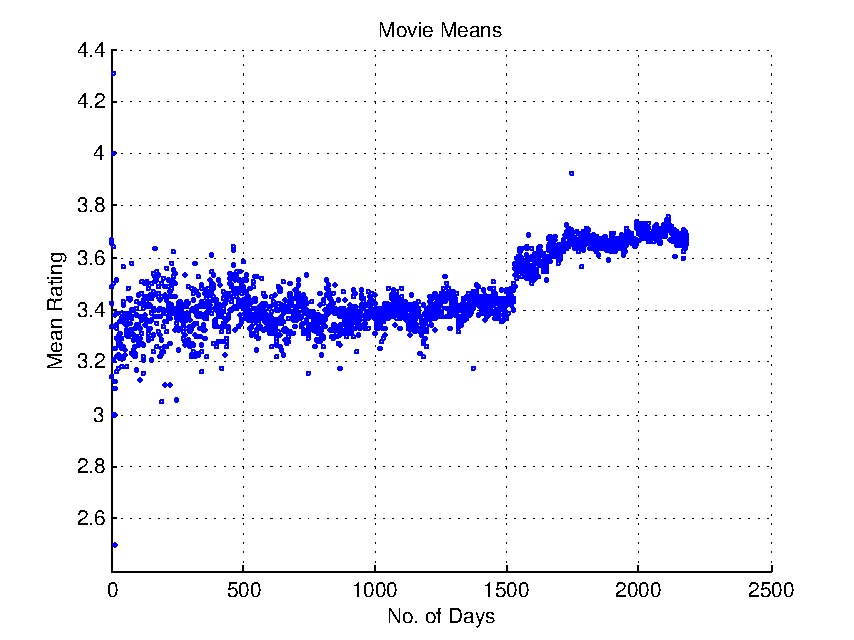
\includegraphics[width=0.45\textwidth]{./New/MovieMeans_AllMovie.pdf}
\label{fig:MovMean}
}
\subfigure[Movie Means by Movie Age]{
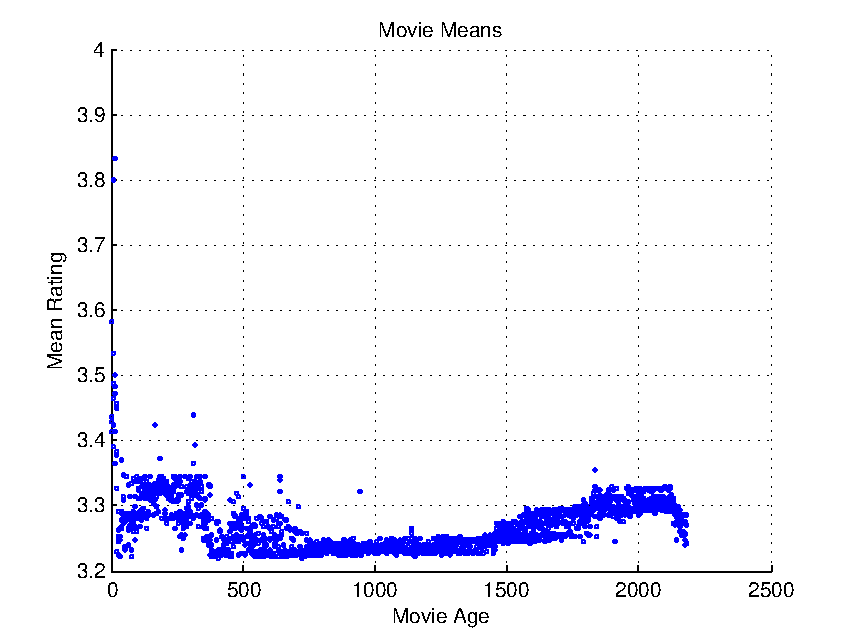
\includegraphics[width=0.45\textwidth]{./New/MovieMeans_AllMovie_Age.pdf}
\label{fig:MovMean_Age}
}\\

\label{fig:MovieMean_temporal}
\caption{Movie Means vs Time}
\end{figure}



\section{Temporal-Factor Model}
As we had seen in the previous chapter, that all the non user-item interaction
effects are encapsulated in the \emph{Baseline predictors}, we will show here
who we intend to include temporal baseline predictors. Here we explain the
theoretical analyses and findings related to various time changing aspects of
users and of movies. It is clear that the time dynamics of movies will be more
gradual than that of the users. The movies are analysed based on a large number
of users who have rated the single movie, but however as an individual user the
temporal analyses is done on large number of unrelated factors, hence the user
behaviour seems more complex and less uniform compared to the movies. \\
The main challenge is to parameterize the user-drift and the movie-drift as
appropriately as possible. The first and foremost consideration is how
transitory are the user-drift and the movie-drift. As we will expalin in detail
the movie-drift seems to be more uniform and less transient than the user-drift,
hence it is wise to consider finer time resolution to model user-drift and
coarser resolution for movies. The final model should however account for both
temporal effects spanning on a longer duration and the more transitory changes. 
For example, movies dont change on a daily basis, some of the factors which
could affect the movies dont occur often like appearance of an actor in another
movie, or the movie winning an award or the movie recieving appreciation from a
critique. On the contrary consider an user, who usually rates relative to other
ratings, so his rating scale could vary everytime he has seen on influencing
movie proir to the current movie of interest. A user who usually rate 4 for
average movies, could be influenced to rate the same kind of average movies by
3. \\

\begin{figure}[h!]
\centering
\subfigure[Monthly Average of All movies]{
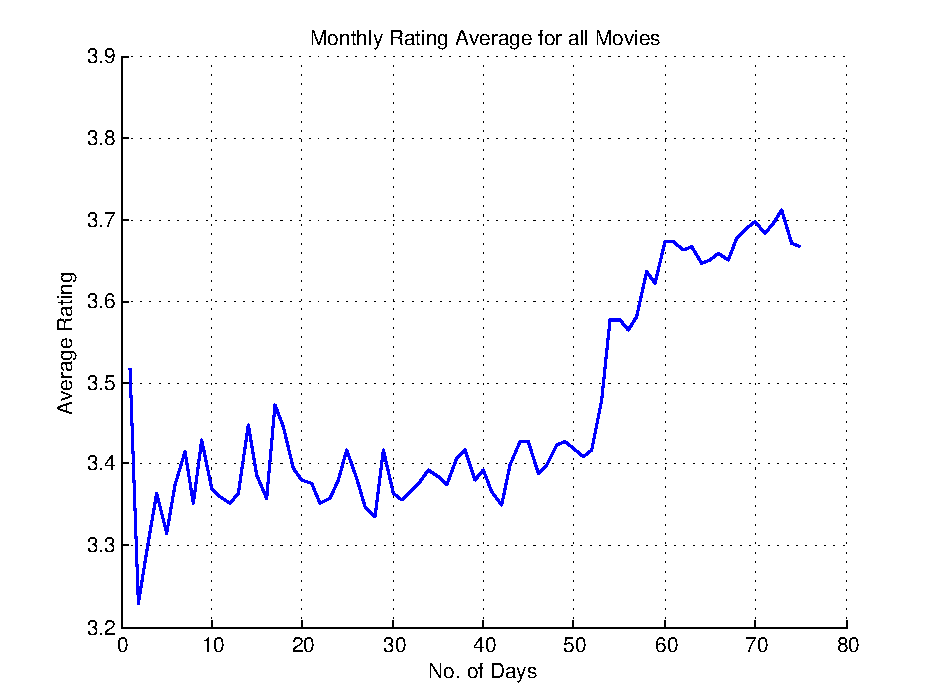
\includegraphics[width=0.45\textwidth]{./New/MonthlyAve_AllMovies.pdf}
\label{fig:MonthlyAllMov}
}
\subfigure[Weekly Average of all movies]{
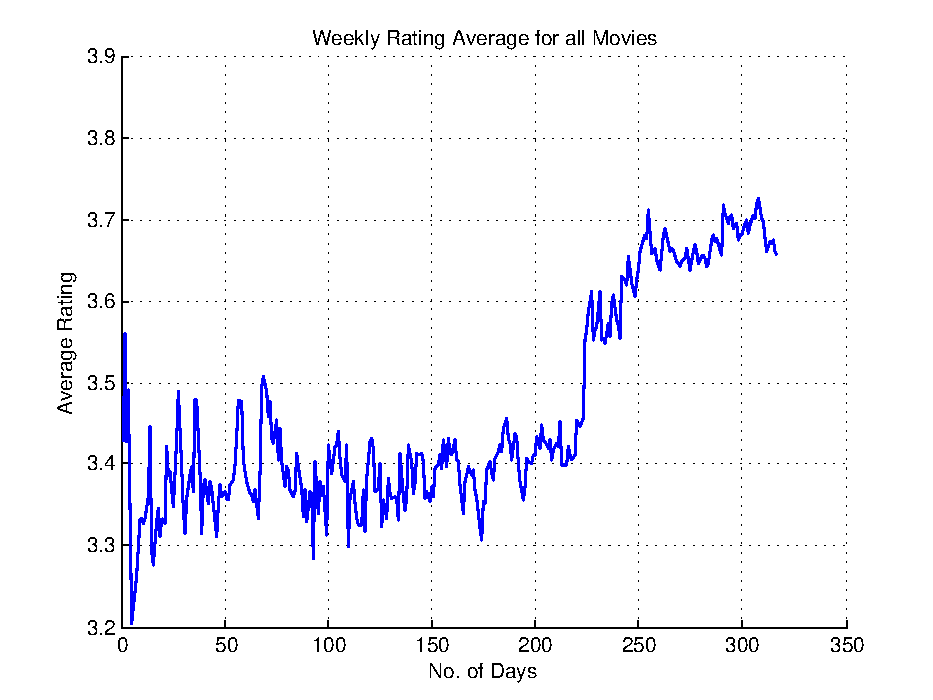
\includegraphics[width=0.45\textwidth]{./New/WeeklyAve_AllMovies.pdf}
\label{fig:WeeklyAllMov}
}\\

\subfigure[Monthly Average of movie 129]{
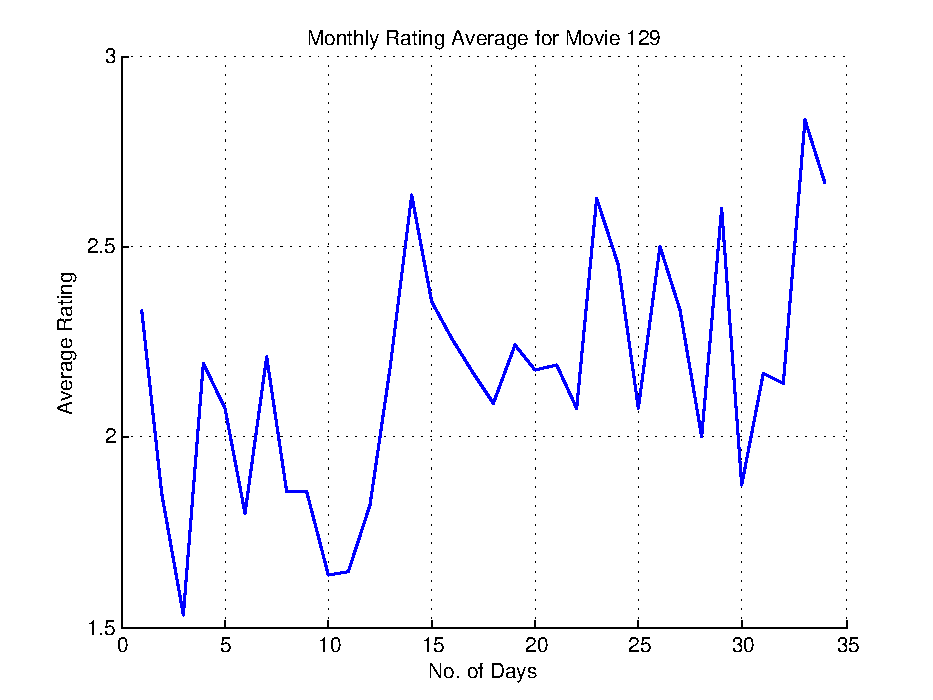
\includegraphics[width=0.45\textwidth]{./New/MonthlyAve_M129.pdf}
\label{fig:MonthlyM129}
}
\subfigure[Weekly Average of movie 129]{
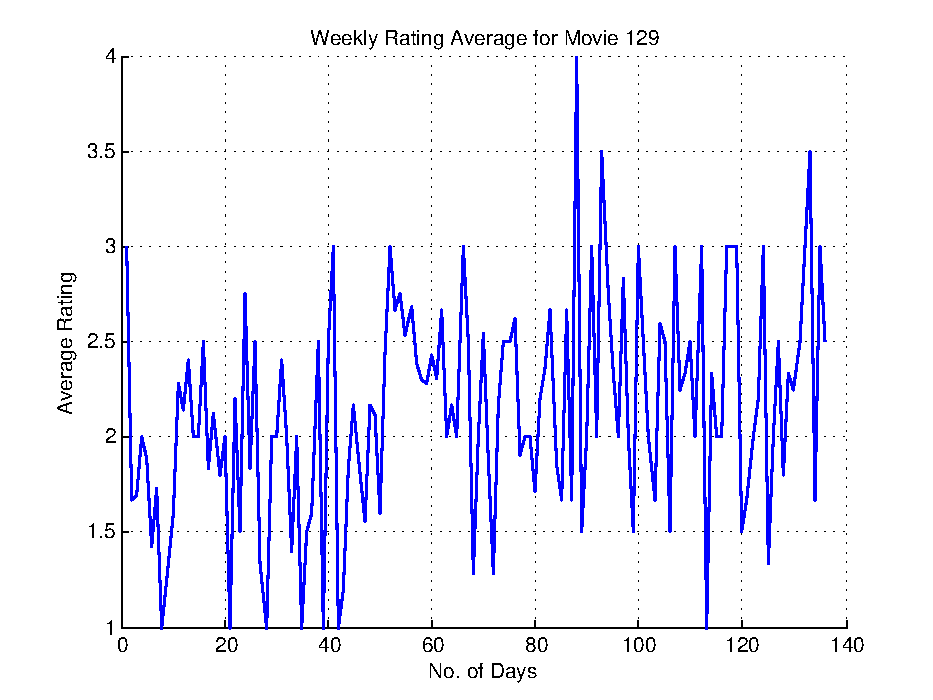
\includegraphics[width=0.45\textwidth]{./New/WeeklyAve_M129.pdf}
\label{fig:WeeklyM1476}
}\\

\subfigure[Monthly Average of movie 1476]{
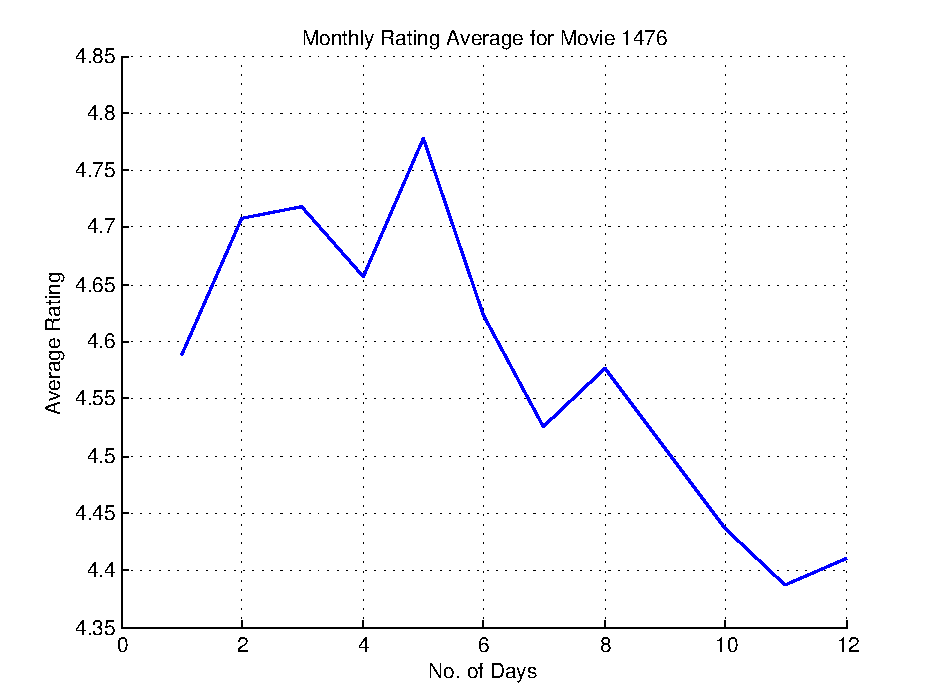
\includegraphics[width=0.45\textwidth]{./New/MonthlyAve_M1476.pdf}
\label{fig:MonthlyM129}
}
\subfigure[Weekly Average of movie 1476]{
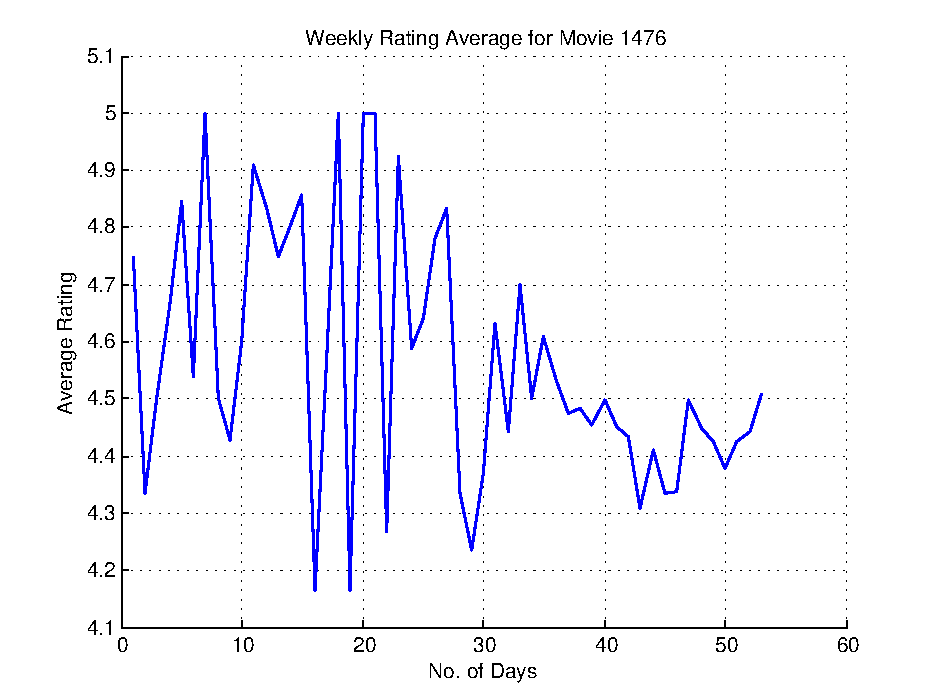
\includegraphics[width=0.45\textwidth]{./New/WeeklyAve_M1476.pdf}
\label{fig:WeeklyM1476}
}\\

\label{fig:MonthlyWeeklyAverages}
\caption{Monthly and Weekly Averages}
\end{figure}

We begun by experimenting for different time periods called \emph{bins} in order
to catch the movie-drifts.  The whole time period spans over 300 weeks, and
after several rounds of testing a 10 week period was chosen as the optimal bin
length. Hence a total of 30 bins suffice to span the entire data. With each bin
we associate it with a bias(transient part), which is simply the difference
between the overall movie mean and the mean of the movie for that bin period.
Interpolation is done for bins where there are no ratings. Each rating instance
of a movie in the training data is associated with a bin value between 1 and 30.
Hence the movie bias would have two components a stationary part, $b_{i}$ and a
transient part $b_{i,Bin(t)}$ \refname{[7]}. \\

\begin{equation} 
 b_{i}(t)=b_{i}+b_{i,Bin(t)}
\end{equation}

We have in this thesis work considered only movie related temporal dynamics,
however we would comment on a possible approach to capture temporal dynamics
related to the more complicated user bias. In case users we need to parameterize
for both long term and short term changes. A simple linear function could be
used to capture the gradual user-bias drift. Each user will have an average
rating date, and for every rating instances of this user the deviation could be
a function of the difference of the dates. Regarding sudden drifts, we need to
capture the drift on daily basis. The minimum step length could be larger than a
day also. In the NETFLIX data the user on an average rates on 40 different days,
hence we need 40 different paramaters for every user on an average. These two
factors could model the temporal dynamics of the users.  




\chapter{Mathematical Background\index{Mathematical Background}}

\textsf{ In this chapter we provide the mathematical proofs which form the basis
of the prediction models. The main concept of matrix factorization is explained
mathematically. Singular value decomposition is explained in detail, and some
issues regarding the disadvantages in the present scenario is explained. An
substitute method Alternate Least Squares is explained. And lastly low rank
approximation is explained.}

\section{Introduction to Matrix Factorization}
Since this chapter is dedicated to the mathematical principles that drives the
prediction models, we can begin with a direct statement, the data matrix is
factorized into simpler matrices which are constrained on its dimensionality.
Different types of constraints can be imposed on the factorization, but for the
particular machine learning task of collaborative filtering we have only used
the low rank approximation. Collaborative filtering can be considered as
\emph{matrix completion} problem, where we are trying to fill in the missing
entries of the sparsely filled rating matrix $R$ $\in\mathbb{R}^{u,i}$. We
complete the rating matrix by approximating it to a full matrix $\hat{R}=PQ'$,
where $P \in\mathbb{R}^{u,k}$ and $Q \in\mathbb{R}^{i,k}$. 

$P$ and $Q$ are unconstranied \emph{factor matrices} and we will show that if
$\hat{R}$ is the best approximation of the original rating matrix, then the
\emph{rank} of $\hat{R}$ is at most $k$. 

Now that we have had a fair idea of how to approach the problem, the next
important concern is to decide in what sense do we want to approximate the data
matrix, or how do we measure the discrepency between the original matrix and the
approximated matrix. The simplest way would be to measure the \emph{Frobenius
distance} between the two,
\[
 \|{R-\hat{R}}\|_{F}^2 = \sum_{ui}^{}(R_{ui}-\hat{R}_{ui})^2
\]
But we use the Root Mean Squared Error(RMSE) to measure the accuracy. 

There might also be a necessity in applicatons like clustering to impose a
constraint on the factored matrices other than only on rank of approximating
matrix. Since clustering is based on some kind of distance measure and distance
can never be negative, it is obvious that we need to impose a non-negative
constraint on the factored matrices. In such cases we cannot rely on SVD as it
can generate negative elements. Instead we might want to compute the rank-$k$
approximation in the following way \cite{eld-mm:07}, \\
\[
  A\approx WH,		W,H\geq0
\] \\

\section{Matrix approximation using SVD}
\begin{theorem}[SVD]
 Any $m \times n$ matrix A with rank k, with $m \geq n$, can be factorized \\
\begin{equation}
  A = U\begin{pmatrix}\Sigma\\0\end{pmatrix}V^{T},
\end{equation}
where $U \in \mathbb{R}^{m \times m}$ and $V \in \mathbb{R}^{n \times n}$, and
$\Sigma \in \mathbb{R}^{m \times n}$ is a diagonal matrix, i.e., $\Sigma =
diag(\sigma_1,\sigma_2,...\sigma_n)$, with $\sigma_1 \geq \sigma_2 \geq ... \geq
\sigma_n \geq 0$. Here $\sigma_1,...,\sigma_n$ are called singular values of A.
The column vectors of U and V are called the right and left singular vectors of
A, respectivley.  
\end{theorem}
The matrix A can be constructed from the singular values as shown below, \\
\begin{equation}
 A=\sum_{i=1}^{n}\sigma_i u_i v_i^T
\end{equation}
The matrix $U$ can be written as $U=[U_1 U_2]$, where $U_1 \in \mathbb{R}^{m
\times n}$. We can obtain the matrix $A$ by the \emph{outer} \emph{product}
\emph{form} in a thin version as shown below,
\[
 A=U_1 \Sigma V^T = \begin{pmatrix}u_1&u_2&\cdots&u_n\end{pmatrix}
  \begin{pmatrix}
  \sigma_1 &         &        &        \\
           & \sigma_2&        &        \\
           &         & \ddots &        \\
           &         &        & \sigma_n
 \end{pmatrix}
 \begin{pmatrix}v_1^T\\v_2^T\\\vdots\\v_n^T\end{pmatrix}\\
\] \\
Now moving ahead with matrix approximation, let us consider our original matrix
$A$, as sum of a low-rank matrix and a small noise, $A_0 + N$. Since it is an
approximation problem we will try to minimise the noise $N$, by estimating the
\emph{correct rank} of $A_0$, this rank is known as \emph{numerical rank}.
\cite{eld-mm:07}. Now the approximation looks like this, \\
\[
 A = \sum_{i=1}^{n}\sigma_i u_i v_i^T \approx \sum_{i=1}^{k}\sigma_k u_k v_k^T
\]\\
\begin{theorem}[Eckart-Young theorem]
 For a matrix A $\in \mathbb{R}^{m \times n}$, with $rank(A)=r>k$. The Frobenius
norm of the matrix approximation problem \\
\begin{equation}
 \min_{rank(\hat{A})=k}\|{A-\hat{A}}\|
\end{equation}\\
which has the solution of 
\begin{equation}
 \hat{A}=U_k \Sigma_{k} V_k^T,
\end{equation}\\
where $U_k = \begin{pmatrix}u_1&u_2&\cdots&u_k\end{pmatrix}$, $V_k=
\begin{pmatrix}v_1^T\\v_2^T\\\vdots\\v_n^T\end{pmatrix}$ and
$\Sigma_k=diag(\sigma_1,\sigma_2,...,\sigma_k)$. Equation 4.3 has the minimum
solution of
\begin{equation}
 \|{A-\hat{A}}\|_{F}=\left(\sum_{i=k+1}^{p}\sigma_i^2\right)^{1/2},
\end{equation}
where $p=min(m,n)$.
\end{theorem}

\section{Matrix approximation using Alternating Least Squares}
\subsection{Disadvantage of SVD}
In this thesis work we have done the implementation using MATLAB, and we use the
function $[U,S,V]=svds(A,k)$ to obtain the singular value decomposition of a
sparse matrix $A$ of rank $k$. However elegant is the method of $SVD$, it
unfortunately fails to produce good predictions. The $SVD$ approximates a rating
matrix by minimizing the \emph{Frobenius norm} of $|R-\hat{R}|$. This is
equvivalent to minimizing the RMSE between individual elements in the rating
matrix. Since the majority of the elements are \emph{unknowns}, and it is our
belief that MATLAB while calulating \emph{SVD} considers these \emph{unknowns}
as zeros, whereas these are not zeros and hence this approach is flawed.
In the Appendix A, we give a detailed explanation as to why SVD is not
appropriate to find the low-rank matrix approximation in our case, where our
data matrix is very sparse($1\%$-dense). 

\subsection{Problem formulation w.r.t ALS}

This approach is based on the article \cite{Zhou:2008:LPC:1424237.1424269}.
Let $U=[\bold{u_i}]$ be the user feature matrix where $\bold{u_i} \subseteq
\mathbb{R}^{n_f}$ and $i=1,2,...,n_u$, and let $M=\bold{m_j}$ be the item or
movie feature matrix, where $\bold{m_j} \subseteq
\mathbb{R}^{n_f}$ and $j=1,2,...,n_m$. Here $n_f$ is the number of factors,
i.e., the reduced dimension or the lower rank, which is determined by cross
validation. The predictions can be calculated for any user-movie combination
$(i,j)$, as $r_{ij}=\bold{u_i} \cdotp \bold{m_j}, \forall i,j$. Here we minimize
the loss function of $U$ and $M$ as the condition in the iterative process of
obtaining these matrices. Let us start by considering the loss due to a single
prediction in terms of sqaured error: 
\begin{equation}
 \mathcal{L}^2(r,\bold{u},\bold{m})=(r-<\bold{u},\bold{m}>)^2.
\end{equation}

Based on the above equation generalizing it for the whole data set, the
\emph{empirical} total loss as:
\begin{equation}
 \mathcal{L}^{emp}(R,U,M)=\frac{1}{n} \sum_{(i,j) \in
I}\mathcal{L}^2(r_{ij},\bold{u_i},\bold{m_j}),
\end{equation}
where $I$ is the known ratings dataset having $n$ ratings. 

Based on the above, we can formulate our low rank matrix approximation problem
as 
\begin{equation}
(U,M)=arg \min_{(U,M)}\mathcal{L}^{emp}(R,U,M).
\end{equation}

Here the number of elements or free parameters we need to determine is $(n_u +
n_m)n_f$, but in our initial known data matrix, .i.e, $R$ we only have $1\%$ of
$n_un_m$ elements. While solving Eq. (4.8) with a sparse $R$ matrix leads to
overfitting. To avoid this we use Tikhonov regularization, our emperical loss
term get another term as shown below:
\begin{equation}
 \mathcal{L}_{\lambda}^{reg}=\mathcal{L}^{emp}(R,U,
M)+\lambda(\|U\Gamma_U\|^2+\|M\Gamma_M\|^2),
\end{equation}
where $\Gamma_U$ and $\Gamma_M$ are Tikhonov matrices. In the next section we
will discuss in detail about how to form these Tikhonov matrices.
\subsection{Regularized ALS}

According to the article \cite{Zhou:2008:LPC:1424237.1424269}, it is best to use
weighted-$\lambda$-regularization, which is as shown below:
\begin{equation}
 f(U,M)= \sum_{(i,j) \in I}(r_{ij}-\bold{u}_i^T\bold{m}_j)^2+\lambda(\sum_i
n_{u_{i}}\|\bold{u}_i\|^2+\sum_j n_{m_{j}}\|\bold{m}_j\|^2),
\end{equation}
The above equation can is somewhat an vectorized version of Eq. (4.9), where the
Tikhonov matrices are replaced by $n_{u_{i}}$ and $n_{m_{j}}$, which are nothing
but the number of ratings of user $i$ and movie $j$. Below equations show how
these terms are related to Tikhonov matrices:
$$\Gamma_U=diag(n_{u_{i}})		\Gamma_M=diag(n_{m_{j}})$$
Now we will discuss how to solve for matrices $U$ and $M$, this is the
mathematical explanation of what was explained under Temporal Bias + ALS model
in Sec. (2.3.3). The matrix $U$ is approximated column wise, i.e., $u_i$, is
determined by solving the regularized least squares problem, using the known
ratings vector of user $i$ and the feature vectors $m_j$, which are the columns
of $M$ matrix corresponding to the movies seen by the user $i$. Let us
represent 
Eq. (4.10), is a simple differential equation style as follows:
\begin{equation}
 f(u,m)=(r-um)^2+\lambda(nu^2+nm^2)
\end{equation}
to minimize this function we equate the first partial differential w.r.t $u$ of
the function $f$ to $0$.
\begin{align}
& \frac{1}{2} \frac{\partial f}{\partial u_{ki}} = 0, & \forall i,k \\
 \implies & \sum_{j\in I_i}(\bold{u}_i^T\bold{m}_j-r_{ij})m_{kj}+\lambds
n_{u_{i}}u_{ki}=0, & \forall i,k \\
 \implies & \sum_{j\in I_i}m_kj\bold{m}_j^T\bold{u}_i
+\lambda n_{u_{i}}u_ki = \sum_{j\in I_i}m_{kj}r_{ij}, & \forall i,k \\
\implies & (M_{I_{i}}M_{I_{i}^T}+\lambda
n_{u_{i}}E)\bold{u}_i=M_{I_{i}}R^T(i,I_i), & \forall i,k \\
\implies & \bold{u}_i = A_{i}^{-1}V_i, & \forall i \\
  \end{align}

where $E$ is $n_f \times n_f$ identity matrix, $V_i=M_{I_{i}}R^T(i,I_i)$ and
$A_i=M_{I_{i}}M_{I_{i}}^T+\lambda n_{u_{i}}E.$ 

Now in the same way by starting with a known $U$ matrix, the movie feature
matrix $M$ is approximated by computing the individual column vectors of $M$ as
shown below: \\
\begin{align*}
 & \bold{m}_j=A_{j}^{-1}V_j, & \forall j,
\end{align*}
where $A_j=U_{I_{i}}U_{I_{i}}^T+\lambda n_{m_{j}}E$ and $V_j=U_{I_{i}}R(I_j,j)$.
$U_{I_{i}}$ is the sub-matrix of $U$, where only $i \in I_j$ are selected.
$R(I_j,j)$ is the column vector which is obtained from the rating matrix $R$, by
selecting all the elements from column $j$ and rows corresponding to $i \in I_j$

\section{Evaluation Metrics}
With the advent of the NETFLIX Competition, \emph{accuracy} has become one of
the most important defining properties of Recommender systems. Hence it is
worthwhile to discuss about different methods of measuring accuracy. The choice
of metrics for accuracy might depend on the kind of systems under study, like if
it is \emph{rating prediction system} or \emph{decision support system}. For the
former we can use statistical accuracy measures where we compare the predicted
value with known actual values, for example the \emph{MAE(Mean Absolute Error)},
\emph{RMSE}, \emph{Correlation} etc. In the case of decision support systems,
where it is required to produce a list of high-relevance items, like in the
\emph{top-N} recommendation systems, the metrics used to measure accuracy are
\emph{precision}, \emph{recall}, or \emph{F-measure} etc. 

\subsection{Mean Average Error}
Let us consider, $\mathcal{T} = \{r_{ij} \exists \mbox{ in } Q_{\text{test}}
\mid \mbox{user } i
\in \mathcal{U} \mbox{ have rated movie } j \in \mathcal{M} \}$, to be the test
set. Then the MAE can be defined as,
\begin{equation}
 MAE = \sum_{r_{i,j}\in{\mathcal{T}}}\frac{|\hat{r}_{ij}-r_{ij}|}{|T|}
\end{equation}
where $\hat{r}_{ij}$ is the predicted rating and $r_{ij}$ is the actual rating,
and $|T|$ is the size of the test set. The goal is to minimize this value to get
better accuracy.

\subsection{RMSE}
For the same test set as shown above, the RMSE is defined as, 
\begin{equation}
  RMSE =\left(
\frac{\sum_{r_{i,j}\in{\mathcal{T}}}{(\hat{r}_{ij}-r_{ij})^2}}{|T|}\right)^{1/2}
\end{equation}

\subsection{Correlation}
If we consider the predicted and the known values to be vectors, then the
correlation gives the proximity of the two vectors. \emph{Pearson Correlation
Coefficient} is an example, which is defined by
\begin{equation}
 \rho_{\hat{r},r}=\frac{cov(\hat{r},r)}{\sigma_{\hat{r}}\sigma_r}
\end{equation}
Higher the value better the accuracy in this case. Geometrically this can be
viewed as the \emph{cosine} of the angle between the two vectors. 

\subsection{Precision and Recall}
In the general \emph{Information retireval} point of view, the precision is
defined as,
\begin{equation}
 P=\frac{D_r}{D_t}
\end{equation}
where $D_r$ is the number of relevant documents retrieved and $D_t$ is the total
number of documents retrieved \cite{eld-mm:07}. But in the
Recommender system point of view the documents are replaced by items, and the
user interest according to the user profile is used instead of the explicit
query. 

Recall is defined as,
\begin{equation}
 R=\frac{D_r}{N_r}
\end{equation}
where $N_r$ is the total number of relevant documents in the database, which in
the case of recommender systems would be the total number of items in the whole
data.

\subsection{F-Measure}
This is a way to combine the precision and recall into one metric, a simple F-1
measure is the harmonic mean of precision and recall. 













\chapter{Results\index{Results}}


\textsf{In this chapter we present the results of the epxeriments conducted,
reasoning the motivation towards the built models. We also talk about aspects
which were considered but not implemented.}

\section{Overview of Different Models}
The principles behind designing the model are firstly, to accurately account for
biases of various types and secondly, formulation of an efficient low-rank
matrix approximation method. The first principle involves identifying different
biases, like, the user-bias, movie-bias and temporal biases w.r.t users and
movies. These biases are the non-interacting parts between the users and movies,
and they are encapsulated into the baseline predictor. These values are
initially subtracted from all the known ratings. They will be integrated back
into the factor model for the new predicted ratings. We have experimented with
three types of biasing techniques, first without any bias, second, with only
static bias, and third, with temporal movie biases. Moving ahead to the
factorization itself, we start with the SVD technique and owing to the
issue of the MATLAB method svds treating the unknown ratings as zeros, we
develop a new factorization technique based on
weighted ALS. Within the ALS algorithm we have two types of initialization
methods, hence leading to ALS-I and ALS-II. The table below shows the various
models built by combining the different biasing and factorizing techniques
mentioned.


\begin{table}
\begin{center}
 
     \begin{tabular}{|c|c|c|c|}
       \hline
        & SVD & ALS-I & ALS-II \\ \hline
       None & Model 1 & Model 6 & Model 7\\        
       $NonTemp_{mu}$ & Model 3 & - & Model 8\\
       $Temp_{mu}$ & Model 2 & - & Model 9\\
       $NonTemp_b$ & - & Model 4 & -\\
       $Temp_b$ & - & Model 5 & -\\ \hline
    \end{tabular}
    \caption{Different Model}     
\end{center}
\end{table}

\subsubsection{SVD}
While using this method, which is [U,S,V]=svds(R,n), where $R$ is the Rating
matrix and $n$ is the rank of the approximating matrix. We test the models for
different values of $n$, the maximum being $n$=200. 

\subsubsection{ALS-I}
This is the type-I ALS method, where the M matrix is initialized by replacing
the assigning the first row with the mean values of the movies, and filling in
random values at the remaining places. 



\begin{enumerate}
 \item Initialize the M matrix, by assigning the means of movies as
the first row entry, and small random numbers in the remaining entries. 
 \item  With this M, solve for U in order to minimize the loss
function.
 \item Now Keep the U matrix from step 2 fixed, and update the M
matrix.
 \item Repeat these iterations until required convergence criteria
is met.
\end{enumerate}


\subsubsection{ALS-II}
This is the type-II ALS method, where the M matrix is initialized by doing an
SVD on the initial rating matrix R, as shown below:

\begingroup
\begin{center}
\begin{align*}
& [U1,S1,V1]=svds(\hat{R},100) \\
& M=S1*V1' 
\end{align*}
\caption{SVD Initialization of M}
\end{center}
\endgroup


\begin{enumerate}
 \item Initialize the M matrix as shown above row entry, and small random
numbers in the remaining
entries. 
 \item With this M, solve for U in order to minimize the loss
function.
 \item Now Keep the U matrix from step 2 fixed, and update
the M matrix.
 \item Repeat these iterations until required convergence
criteria is met.
\end{enumerate}

\subsubsection{$NonTemp_{mu}$}
This is the non-temporal model with the mean of all movies included in it, it is
given by \\
\begin{equation}
 b_{ui}=\mu+b_u+b_i
\end{equation}
where $b_{ui}$ is the baseline predictor, which encapsulates the non-interacting
parts of user-item relationship, $\mu$ is the mean of all movies which is
$3.6043$, $b_u$ and $b_i$ are the observed deviations from the mean. 

\subsubsection{$Temp_{mu}$}
This is the baseline predictor which involves the tie-changing movie biases,
$b_{i,Bin(t)}$.
\begin{equation}
 b_{ui}=\mu+b_u+b_i+b_{i,Bin(t)}
\end{equation}

\subsubsection{$NonTemp_b$}
This is again non-temporal model, but without the all movie mean $\mu$. This
model is only used in conjuction with the ALS-I method, as in this method the
means is already included into the model during the initialization of M.
\begin{equation}
 b_{ui}=b_u+b_i
\end{equation}

\subsubsection{$Temp_b$}
This is the temporal model without the all movie mean $\mu$, again used for
ALS-I but with time-changing movie biases,
\begin{equation}
 b_{ui}=b_u+b_i+b_{i,Bin(t)}
\end{equation}

\section{Results}
\begin{figure}[h!]
\centering
\subfigure[RMSE for Model 1]{
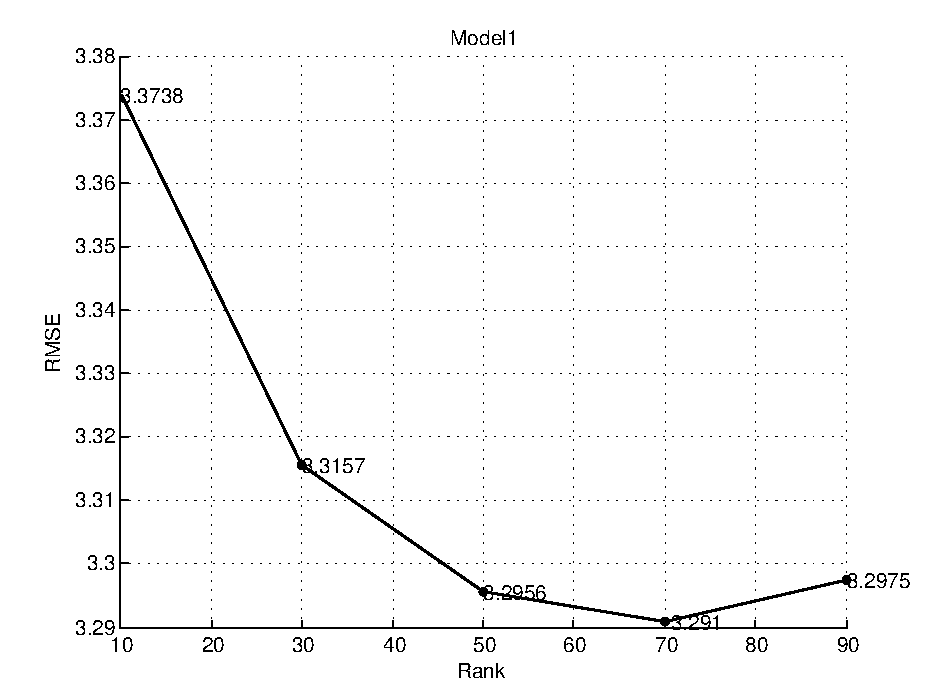
\includegraphics[width=0.45\textwidth]{./Results/plots/model1.pdf}
\label{fig:Model 1}
}
\subfigure[RMSE for Model 2]{
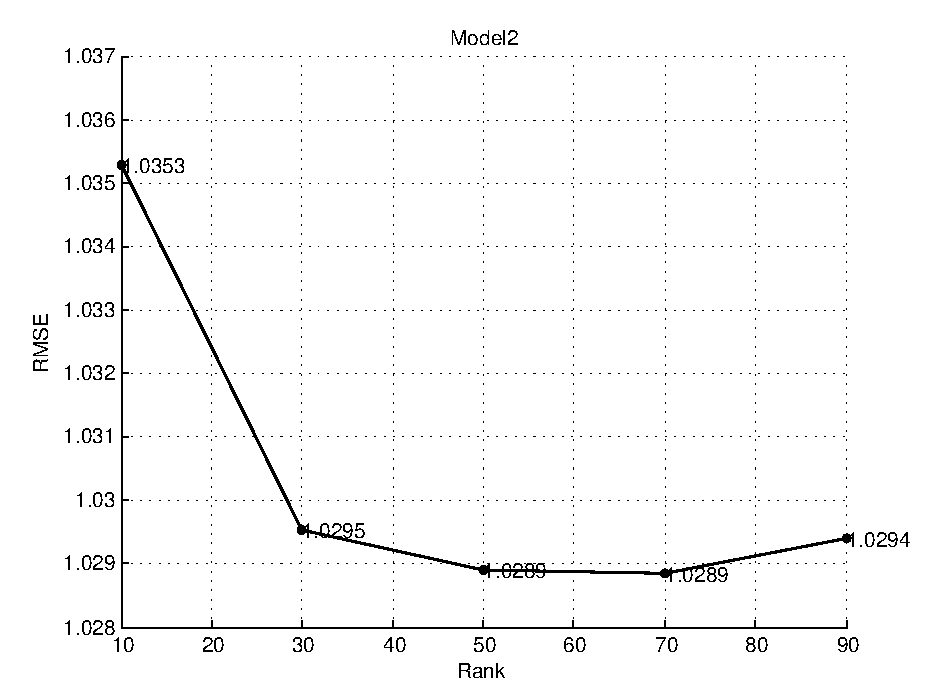
\includegraphics[width=0.45\textwidth]{./Results/plots/model2.pdf}
\label{fig:Model2}
}\\
\subfigure[RMSE for Model 3]{
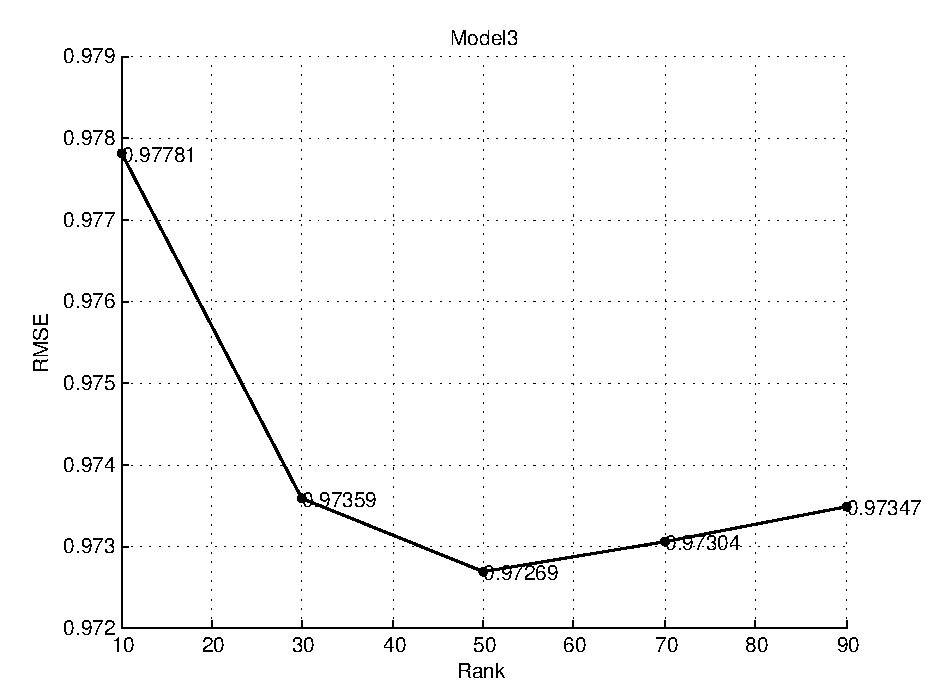
\includegraphics[width=0.45\textwidth]{./Results/plots/model3.pdf}
\label{fig:Model 3}
}
\label{fig:RMSE SVD}
\caption{RMSE: SVD based models}
\end{figure}

In the following figure 5.1, we can see that beyond certain ranks overfitting
occurs. Also we cab observe the improvement in the results by involving the
biases. 

Next we show the results for the ALS based models. Figure 5.2 shows the RMSE of
ALS based models which use the type I initialization technique. 


\begin{figure}[h!]
\centering
\subfigure[RMSE for Model 4 for 30 iterations $N_f=200$]{
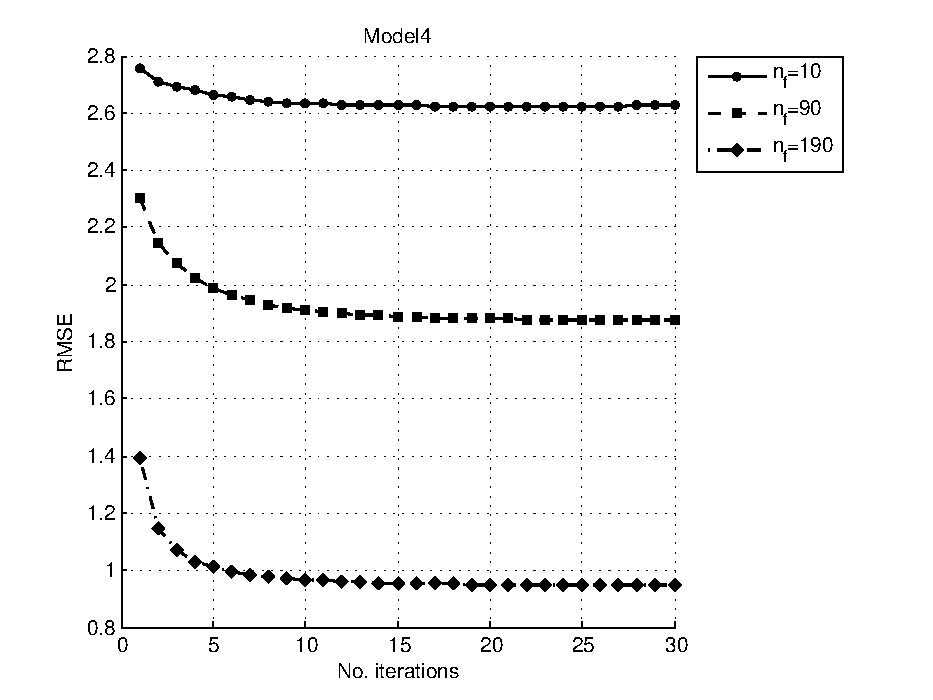
\includegraphics[width=0.45\textwidth]{./Results/plots/model4.pdf}
\label{fig:Model 1}
}
\subfigure[RMSE for Model 4 ]{
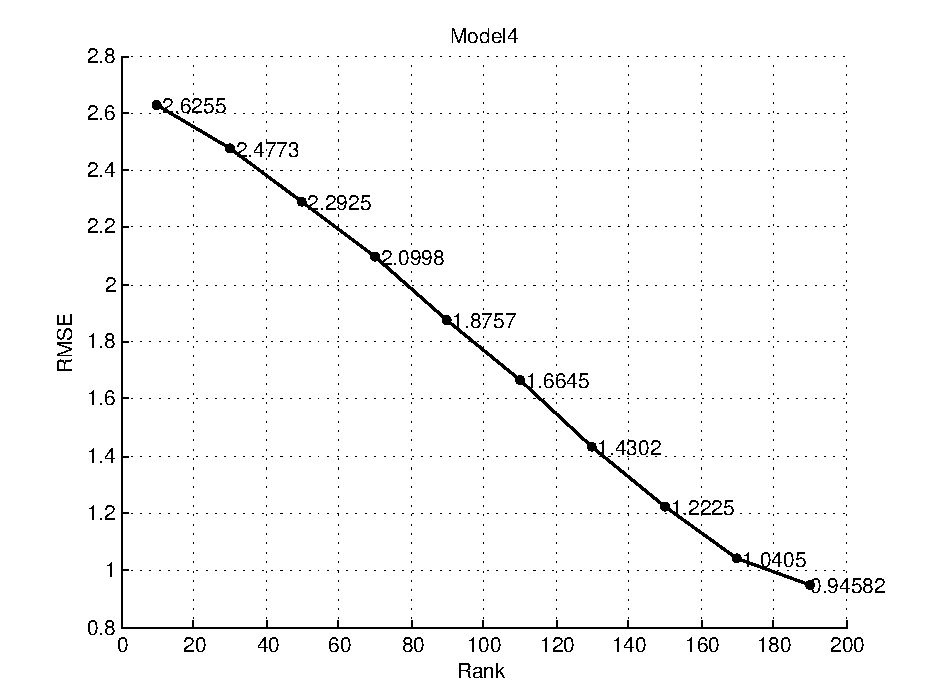
\includegraphics[width=0.45\textwidth]{./Results/plots/model4_1.pdf}
\label{fig:Model2}
}\\
\subfigure[RMSE for Model 5 for 30 iterations $N_f=200$]{
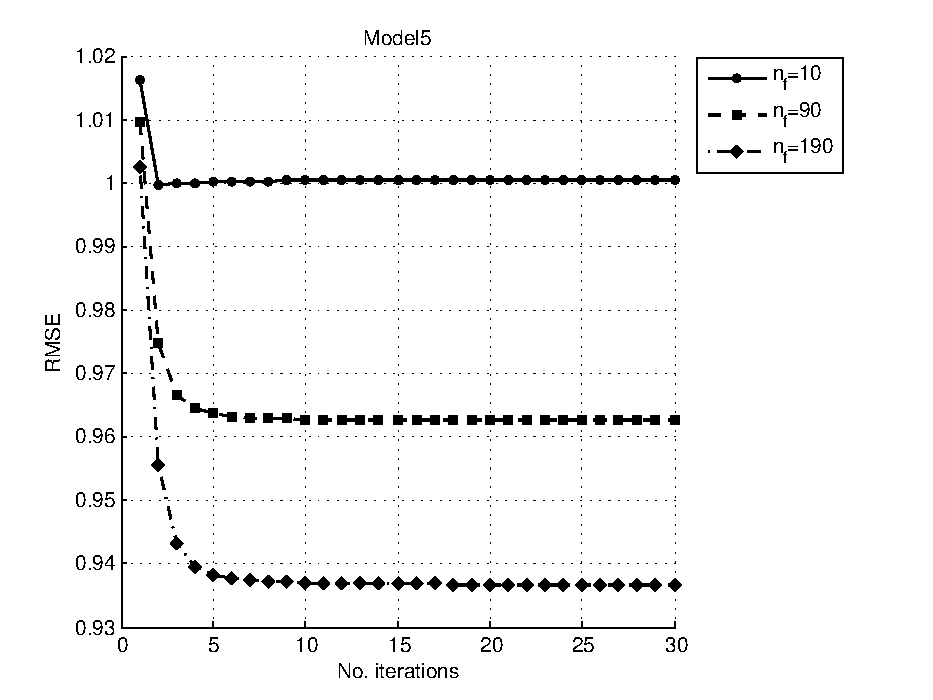
\includegraphics[width=0.45\textwidth]{./Results/plots/model5.pdf}
\label{fig:Model 1}
}
\subfigure[RMSE for Model 5 ]{
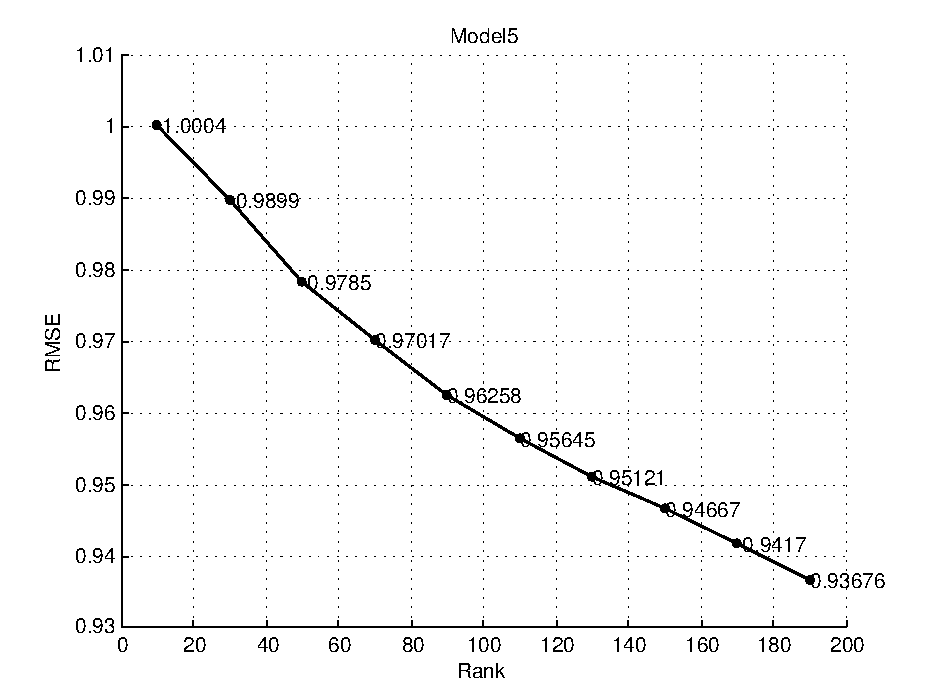
\includegraphics[width=0.45\textwidth]{./Results/plots/model5_1.pdf}
\label{fig:Model2}
}\\
\subfigure[RMSE for Model 6 for 30 iterations $N_f=200$]{
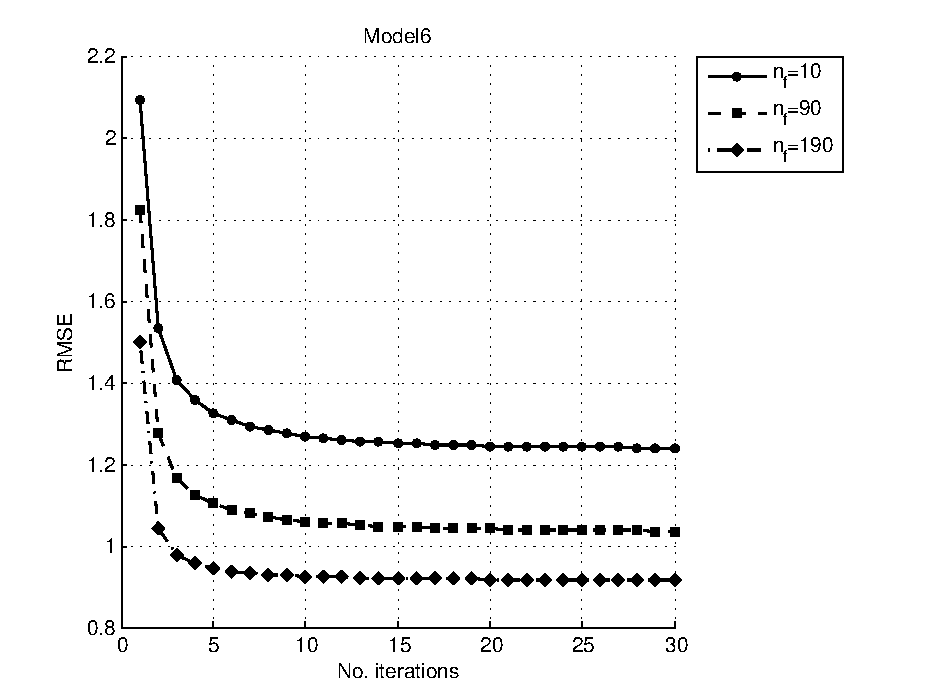
\includegraphics[width=0.45\textwidth]{./Results/plots/model6.pdf}
\label{fig:Model 1}
}
\subfigure[RMSE for Model 6 ]{
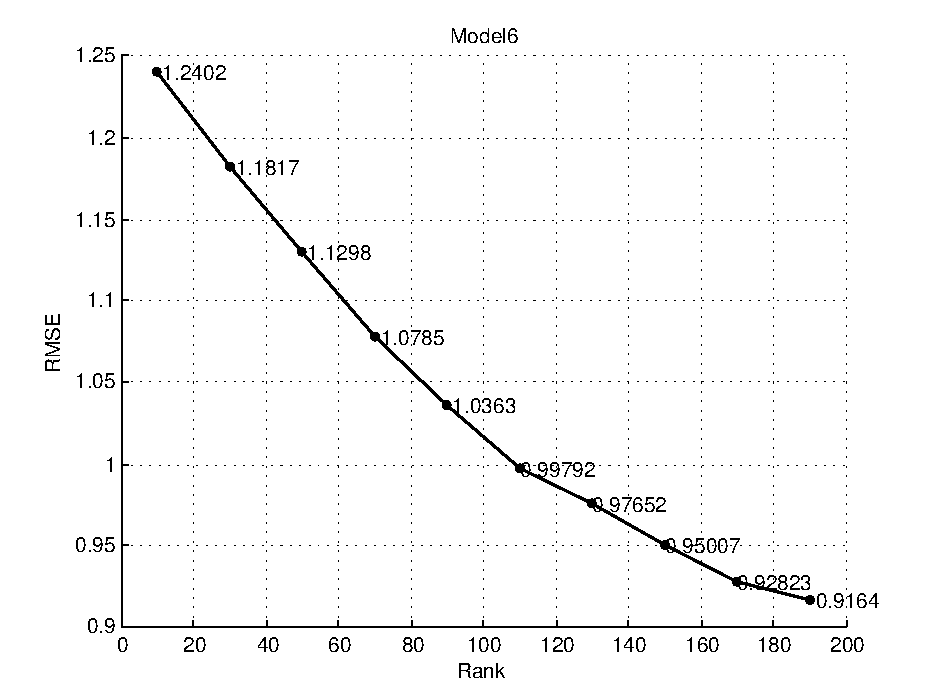
\includegraphics[width=0.45\textwidth]{./Results/plots/model6_1.pdf}
\label{fig:Model2}
}\\
\label{fig:RMSE SVD}
\caption{RMSE: ALS-I based models}
\end{figure}

\begin{figure}[h!]
\centering
\subfigure[RMSE for Model 7 for 30 iterations $N_f=200$]{
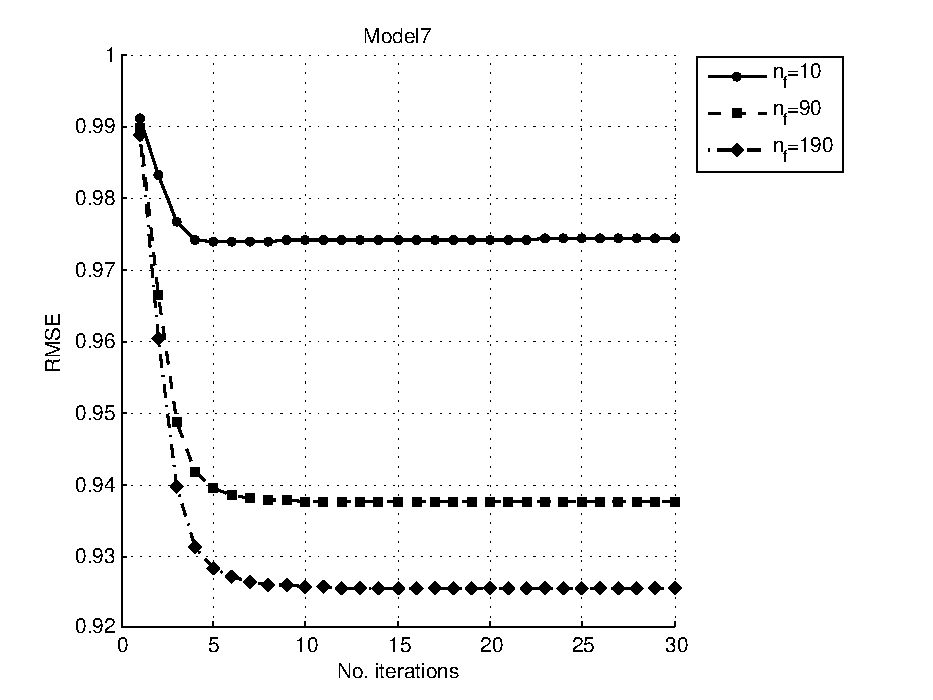
\includegraphics[width=0.45\textwidth]{./Results/plots/model7.pdf}
\label{fig:Model 1}
}
\subfigure[RMSE for Model 7 ]{
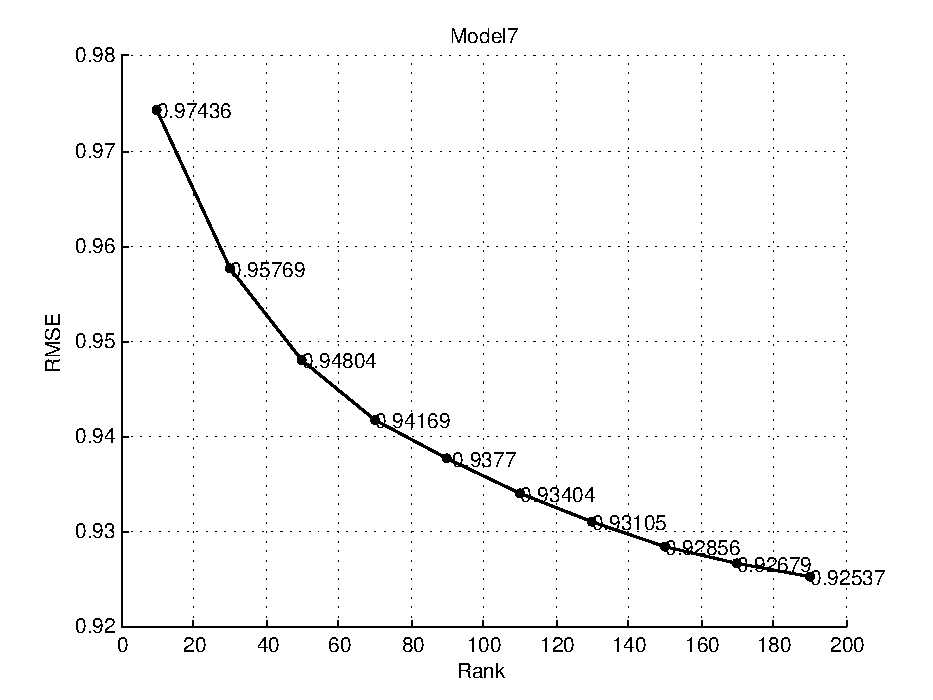
\includegraphics[width=0.45\textwidth]{./Results/plots/model7_1.pdf}
\label{fig:Model2}
}\\
\subfigure[RMSE for Model 8 for 30 iterations $N_f=200$]{
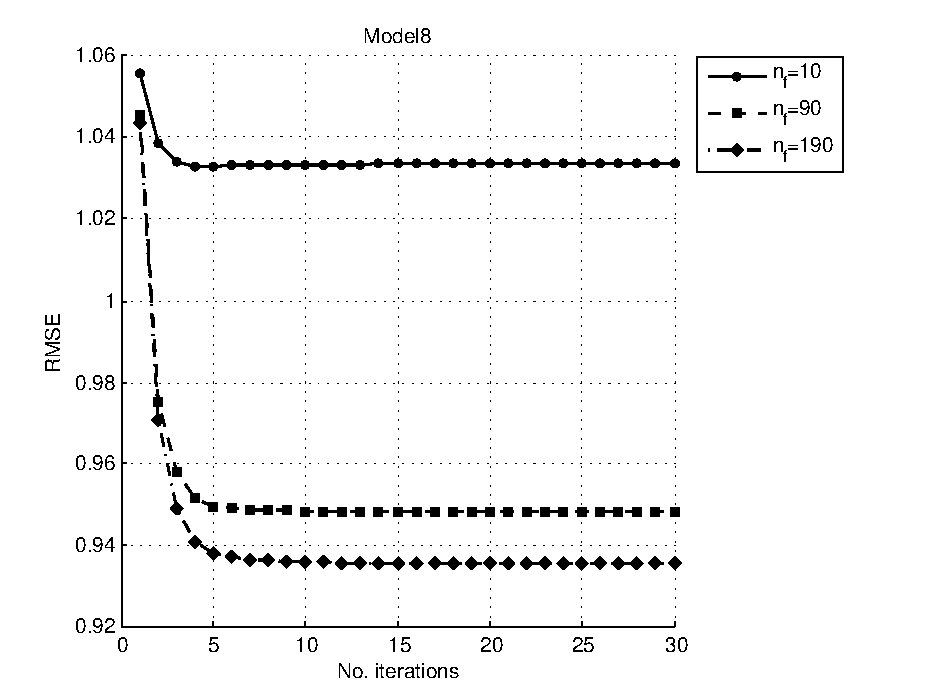
\includegraphics[width=0.45\textwidth]{./Results/plots/model8.pdf}
\label{fig:Model 1}
}
\subfigure[RMSE for Model 8 ]{
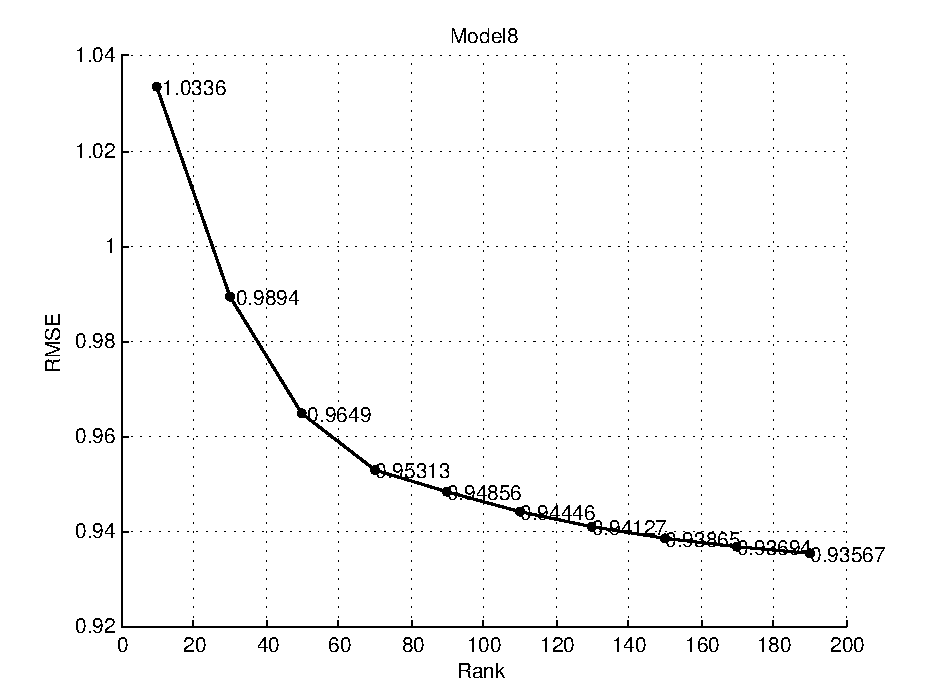
\includegraphics[width=0.45\textwidth]{./Results/plots/model8_1.pdf}
\label{fig:Model2}
}\\
\subfigure[RMSE for Model 9 for 30 iterations $N_f=200$]{
\includegraphics[width=0.45\textwidth]{./Results/plots/model9.pdf}
\label{fig:Model 1}
}
\subfigure[RMSE for Model 9 ]{
\includegraphics[width=0.45\textwidth]{./Results/plots/model9_1.pdf}
\label{fig:Model2}
}\\
\label{fig:RMSE SVD}
\caption{RMSE: ALS-II based models}
\end{figure}


\section{Future Work}
In this work we have only considered only movie related temporal effects. We
could for future work also include the more complex user realted temporal
effects. The user related temporal dynamics proves to be more comples and more
challenging to model. In a single household different people could be involved
in rating movies, and the mood and temperment of the user is susceptible to more
frequent changes. The user rates on forty different days on average. Apart from
the mood swings, the user could also alter the rating scale over time. We could
for further work consider the various user related effects and incude them into
the model in order to get more accurate predictions. 

Owing to the issue of unknown ratings being treated as zeros by the sparse SVD
of MATLAB, we have used an
alternative method. Instead it is possible to develop a factorization technique
based on SVD, but which is regularised. This approach was suggested initially by
Simon Funk \cite{Paterek_RegSVD}.

We could also aim to improve the prediction accuracy by considering inplicit
feedback. By doing so we can take advantage of additional information about user
preferences. In the current system, where we use only explicit ratings, where
there are users for whom we have very little information, implicit data could
prove to be useful \cite{citeulike:8923836}.









\bibliographystyle{plain}
\bibliography{bibl}

\backmatter
\appendix
\chapter{Sparse SVD Computation}
\label{app:SVDS}

\subsubsection{SVDS} 

This function in MATLAB computes the singular vectors and singular values of a given sparse matrix. \\


\subsubsection{Syntax} 

$[U,S,V]=svds(A,k),$ \\
where U is the \emph{right singular vectors} $m \times k$ matrix having orthnormal columns, \\
      V is the \emph{left singular vectors} $n \times k$ matrix having orthnormal columns, \\
      S is the $k \times k$ diagonal matrix, where the diagonal elements are the singular values. \\
      
\subsubsection{Description}
% \begin{left}
% \line(1,0){\textwidth}
% \end{left} \\
The MATLAB function svds uses Lanczos Tridiagonalization on the matrix,
\[
  B = \begin{pmatrix}
   0          &   A            \\
      A^T      & 0     \\

 \end{pmatrix}
\] \\


\begin{algorithm}
\caption{Lanczos tridiagonalization}
\begin{algorithmic}
Initialization: Starting vector $v_1$, such that $||v_1||_2=1$, $\beta_{0}=0$ and $v_0=0$.
 \For{$j=1,2,....$}
  \State$\alpha_{j}=v_j^{T}Av_j$.
  \State$v=Av_j-\alpha_jv_j-\beta_{j-1}v_{j-1}$
  \State$\beta_j=||v||_2$
  \State$v_{j+1}=(1/\beta_j)v$  
 \EndFor
\end{algorithmic}

\end{algorithm}





\end{document}
| returns and the picture is ready. From this point on, the external graphics will be used.

There is another possibility to communicate \meta{main document} to the subprocess performing the externalization: namely to write `|\tikzexternalize{main}|' into the document. In this case, the conversion system call will be
\begin{codeexample}[code only]
pdflatex -jobname "main-figure0" "main"
\end{codeexample}
\noindent and the contents of |\tikzexternalrealjob| is set automatically. This case is detected by |\tikzexternalize|, and the |system call| is updated automatically (by patching its |\texsource| template argument). It is not necessary to change the |system call| manually.


The sequence in which system calls are performed and the decision whether they are issued automatically is governed by the |mode| key, consult its documentation for details.


\subsection{Using External Graphics Without \textmd{\pgfname}\ Installed}
\label{section-libs-external-nopgf}
Given that every picture has been exported correctly, one may want to compile a file without \pgfname\ and \tikzname\ installed. \tikzname\ comes with a minimal package which contains just enough commands to replace every |tikzpicture| environment and the |\tikz| short command with the appropriate external graphics. It can be found at
\begin{codeexample}[code only]
latex/pgf/utilities/tikzexternal.sty
\end{codeexample}
\noindent and needs to be used instead of |\usepackage{tikz}|. So, we uncomment |\usepackage{tikz}| and our example from the beginning becomes
\begin{codeexample}[code only]
\documentclass{article}
% main document, called main.tex
%\usepackage{tikz}

\usepackage{graphicx}
\usepackage{tikzexternal}

%\usetikzlibrary{external}
\tikzexternalize

\begin{document}
\begin{tikzpicture}
  \node {root}
    child {node {left}}
    child {node {right}
      child {node {child}}
      child {node {child}}
    };
\end{tikzpicture}

A simple image is \tikz \fill (0,0) circle(5pt);.

Furthermore, we might want to draw \tikz[baseline]\draw (0,-1) rectangle (1,1);
\end{document}
\end{codeexample}
\noindent where the following files are necessary to compile the document:
\begin{codeexample}[code only]
tikzexternal.sty
main.tex
main-figure0.pdf
main-figure1.pdf
main-figure2.pdf
\end{codeexample}
\noindent If there are any `|.dpth|' files, for example |main-figure2.dpth|, these files are also required. They contain information for the \tikzname\ |baseline| option (or |\label|s inside of external graphics).

Just copy the |.sty| file into the directory of your |main.tex| file and use it as part of your document.

Please keep in mind, that only |tikzpicture| environments and |\tikz| short images are available within the externalization framework. Additionally, calls to |\tikzset| and |\pgfkeys| won't lead to compilation errors because they are simply ignored. But since |pgfkeys| is not available, any option supplied to |\tikzexternalize| is \emph{ignored}.

\paragraph{Attention:} Since the simple replacement |\usepackage{tikzexternal}| doesn't support the key--value interface, you \emph{need} to use |\tikzsetexternalprefix| instead of the |prefix| option and |\tikzsetfigurename| instead of the |figure name| option since |\tikzset| is not available in such a context.

\paragraph{Remark:} Some of the features of this library are mainly useful to improve the speed of successive document compilations. In other words: you can't use all features in this context, Keep it simple.

\subsection{\eps\ Graphics Export}
It is also possible to use \eps\ graphics instead of \pdf\ files. There are different ways to produce them, for example to use |pdflatex| and call |pdftops -eps |\marg{pdf file} \marg{eps file} afterwards. You could add this command to the |system call| option.

Alternatively, you can use |latex| and |dvips| for image conversion as is explained for the |system call| option, see page~\pageref{extlib:systemcall:option}. See the documentation for the basic level externalization in section~\ref{section-external} for restrictions of other drivers.

\subsection{Bitmap Graphics Export}
Occasionally, you may have an extremely large graphics which takes long times to render. It might be interesting to generate a bitmap (raster) image, which displays much faster (for example in a presentation). I have used this feature to speed-up the display of large shadings.

The |external| library can be customized to export bitmap images -- with the help of external programs. Due to the dependence of external programs, you may need to adjust these commands manually. For example, on my computer, the ImageMagick Suite is installed which comes with the |convert| tool. Together with |pdflatex|, I can define the following style:
\begin{codeexample}[code only]
\tikzset{
    % Defines a custom style which generates BOTH, .pdf and .png export
    % but prefers the .png on inclusion.
    %
    % This style is not pre-defined, you may need to copy-paste and
    % adjust it.
    png export/.style={
        external/system call/.add=
            {}
            {; convert -density 300 -transparent white "\image.pdf" "\image.png"},
        %
        /pgf/images/external info,
        /pgf/images/include external/.code={%
            \includegraphics
                [width=\pgfexternalwidth,height=\pgfexternalheight]
                {##1.png}%
        },
    }
}
\end{codeexample}
\noindent The example above defines a new style called `|png export|' which, when it is set with |\tikzset{png export}| somewhere in the document, modifies the configuration for both, file generation and file input. The file generation is modified by appending the ImageMagick command to |system call| (separated by `|;|' as usual on Linux). This is, in principle, enough to generate a |.png| file. The |include external| command is overwritten such that it uses the |.png| file instead of the |.pdf| file (which exists as well in the configuration above). But since a |.png| file can have a much higher resolution than the desired image dimensions, we have to add |width| and |height| explicitly. Usually, the |external| library does not provide size information (it is unnecessary for |.pdf| or |.eps| since these formats have their bounding box information). To enable size information, the style uses the |external info| key which, in turn, provides the |\pgfexternalwidth| and |\pgfexternalheight| commands.

Now, we can use |\tikzset{png export}| either document--wide or just for one particular image. The configuration remains in effect until the end of the actual environment (or until the next closing curly brace `|}|').

\begin{key}{/pgf/images/external info=\mchoice{true,false} (initially false)}
	If this key is activated, the size for any externalized image will be stored explicitly into the associated |.dpth| file.

	When the file is included by |\pgfincludeexternalgraphics| (or automatically by the |external| library), the width is available as \declareandlabel{\pgfexternalwidth} and the height as \declareandlabel{\pgfexternalheight}.
\end{key}

\subsection{Compatibility Issues}
\subsubsection{References In External Pictures}
It is allowed if a picture contains references, for example |\tikz \node {Reference to \ref{a:label}};|.

There is just one issue: if the main job is currently compiling, its |.aux| file is not in its final state (even worse: it may not be readable at all). The picture externalization, however, needs the main |.aux| file to query any references.

Thus, you \emph{will} need to invoke |pdflatex -jobname |\meta{image}| |\meta{mainfile} \emph{manually} for any image which contains references.

This problem arises only for |mode=convert with system call|. In this case,  the |external| library creates a special |\jobname.auxlock| file to check whether the main |.aux| file is currently usable.

\subsubsection{Compatibility With Other Libraries or Packages}
The |external| library has the following compatibility issues:
\begin{enumerate}
	\item The |external| library comes with special support for |\usetikzlibrary{fadings}|: the |fadings| library may define local pictures which would be externalized (although they shouldn't). There is special handling to suppress this bug if |\tikzexternalize| is called \emph{after} |\usetikzlibrary{fadings}| or if all fadings are defined \emph{before} |\tikzexternalize|.

	\item Problems have been reported when using |\tikzexternalize| (or the basic layer externalization) together with |\usepackage{glossary}|. This problem disappears if |\tikzexternalize| is called \emph{before} |\usepackage{glossary}|.

	\item Problems with |\usepackage{pdfpages}| and |\usepackage{vmargin}|: The |external| library replaces the current shipout routine of \TeX\ during its externalization. This might raise problems with other packages which also manipulate the shipout routine (like the mentioned ones).

	To fix those problems, use
\begin{codeexample}[code only]

\usetikzlibrary{external}

\tikzifexternalizing{%
	% don't include package XYZ here
}{%
	\usepackage{pdfpages}
	\usepackage{vmargin}
	...
}%
\end{codeexample}
	This uses the requested packages for the main document, but not for the single, exported graphics.
\end{enumerate}

In general, the |\tikzifexternalizing| feature might be used to solve package conflicts and the |\tikzexternaldisable| and |\tikzexternalenable| features can be used to solve problems with single pictures.

\subsubsection{Compatibility With Bounding Box Restrictions}
Bounding box restrictions provide no problem when used with \eps\ graphics. However, they pose problems for |pdflatex|, so you may need to use the |latex| / |dvips| combination if you use bounding box restrictions and externalization. Currently, the only possibility for bounding box restrictions and |pdflatex| is to use a combination of |trim left| / |trim right| / |baseline|: these keys do not \emph{really} truncate the bounding box, they only store horizontal and vertical shifts (also see the |trim lowlevel| key in this context).

\subsubsection{Interoperability With The Basic Layer Externalization}
This library is fully compatible with |\beginpgfgraphicnamed|$\dotsc$|\endpgfgraphicnamed| environments. However, you will need to use the |export next=false| key to avoid conflicts:
\begin{codeexample}[code only]
\beginpgfgraphicnamed{picture4}
\tikzset{external/export next=false}
\begin{tikzpicture}
   \draw (0,0) -- (4,4);
\end{tikzpicture}
\endpgfgraphicnamed
\end{codeexample}
Please keep in mind that file prefixes do not apply to the basic layer.
}
\endinput
